%%%%%%%%%%%%%%%%%%%%%%%%%%%%%%%%%%%%%%%%%
% Stylish Article
% LaTeX Template
% Version 2.0 (13/4/14)
%
% This template has been downloaded from:
% http://www.LaTeXTemplates.com
%
% Original author:
% Mathias Legrand (legrand.mathias@gmail.com)
%
% License:
% CC BY-NC-SA 3.0 (http://creativecommons.org/licenses/by-nc-sa/3.0/)
%
%%%%%%%%%%%%%%%%%%%%%%%%%%%%%%%%%%%%%%%%%

%----------------------------------------------------------------------------------------
%	PACKAGES AND OTHER DOCUMENT CONFIGURATIONS
%----------------------------------------------------------------------------------------

\documentclass[fleqn,10pt]{SelfArx} % Document font size and equations flushed left

\usepackage{lipsum} % Required to insert dummy text. To be removed otherwise
\usepackage{datetime}

%----------------------------------------------------------------------------------------
%	COLUMNS
%----------------------------------------------------------------------------------------

\setlength{\columnsep}{0.55cm} % Distance between the two columns of text
\setlength{\fboxrule}{0.75pt} % Width of the border around the abstract

%----------------------------------------------------------------------------------------
%	COLORS
%----------------------------------------------------------------------------------------

\definecolor{color1}{RGB}{0,0,90} % Color of the article title and sections
\definecolor{color2}{RGB}{0,20,20} % Color of the boxes behind the abstract and headings

%----------------------------------------------------------------------------------------
%	HYPERLINKS
%----------------------------------------------------------------------------------------

\usepackage{hyperref} % Required for hyperlinks
\hypersetup{hidelinks,colorlinks,breaklinks=true,urlcolor=color2,citecolor=color1,linkcolor=color1,bookmarksopen=false,pdftitle={Title},pdfauthor={Author}}

%----------------------------------------------------------------------------------------
%	MISCELLANEOUS
%----------------------------------------------------------------------------------------
\usepackage{tcolorbox}
\tcbuselibrary{theorems}

\newtcbtheorem[number within=section]{mytheo}{}%
{colback=color1!5,colframe=color1!35!color1,fonttitle=\bfseries}{th}

%----------------------------------------------------------------------------------------
%	ARTICLE INFORMATION
%----------------------------------------------------------------------------------------

\JournalInfo{Zusammenfassung Neuronale Netze SS 2015} % Journal information
\CurrentStatus{Stand: \today, \currenttime Uhr} % Date of last modification
\Archive{} % Additional notes (e.g. copyright, DOI, review/research article)

\PaperTitle{Neuronale Netze} % Article title

\Authors{Benjamin Rupp\textsuperscript{1}*, Sophie von Schmettow\textsuperscript{2}} % Authors
%\affiliation{\textsuperscript{1}\textit{Department of Biology, University of Examples, London, United Kingdom}} % Author affiliation
%\affiliation{\textsuperscript{2}\textit{Department of Chemistry, University of Examples, London, United Kingdom}} % Author affiliation
%\affiliation{*\textbf{Corresponding author}: john@smith.com} % Corresponding author

\Keywords{Keyword1 --- Keyword2 --- Keyword3} % Keywords - if you don't want any simply remove all the text between the curly brackets
\newcommand{\keywordname}{Keywords} % Defines the keywords heading name

%----------------------------------------------------------------------------------------
%	ABSTRACT
%----------------------------------------------------------------------------------------

\Abstract{...}

%----------------------------------------------------------------------------------------

\begin{document}

\flushbottom % Makes all text pages the same height

\maketitle % Print the title and abstract box

\tableofcontents % Print the contents section

\thispagestyle{empty} % Removes page numbering from the first page
%----------------------------------------------------------------------------------------
%	UTILS
%----------------------------------------------------------------------------------------

%\begin{figure*}[ht]\centering % Using \begin{figure*} makes the figure take up the entire width of the page
%\includegraphics[width=\linewidth]{view}
%\caption{Wide Picture}
%\label{fig:view}
%\end{figure*}



%\begin{equation}
%\cos^3 \theta =\frac{1}{4}\cos\theta+\frac{3}{4}\cos 3\theta
%\label{eq:refname2}
%\end{equation}



%\begin{enumerate}[noitemsep] % [noitemsep] removes whitespace between the items for a compact look
%\item First item in a list
%\item Second item in a list
%\item Third item in a list
%\end{enumerate}



%\begin{figure}[ht]\centering
%\includegraphics[width=\linewidth]{results}
%\caption{In-text Picture}
%\label{fig:results}
%\end{figure}

%Reference to Figure \ref{fig:results}.


%\begin{table}[hbt]
%\caption{Table of Grades}
%\centering
%\begin{tabular}{llr}
%\toprule
%\multicolumn{2}{c}{Name} \\
%\cmidrule(r){1-2}
%First name & Last Name & Grade \\
%\midrule
%John & Doe & $7.5$ \\
%Richard & Miles & $2$ \\
%\bottomrule
%\end{tabular}
%\label{tab:label}
%\end{table}



%\begin{description}
%\item[Word] Definition
%\item[Concept] Explanation
%\item[Idea] Text
%\end{description}

%----------------------------------------------------------------------------------------
%	ARTICLE CONTENTS
%----------------------------------------------------------------------------------------
\section*{Disclaimer}
Dieses Dokument wurde im Rahmen des Master-Studiums
für das Modul Neuronale Netze erstellt. Es stellt ei-
ne Zusammenfassung dar und dient zur Vorbereitung auf die
mündliche Prüfung. Neben den Materialien der Vorlesung,
fließen auch weitere Quellen ein, um den behandelten Stoff
auszuarbeiten. Auf den Verweis von Quellen wird verzichtet,
da die Erstellung keinerlei wissenschaftlichen Zweck verfolgt
und nur für den privaten Gebrauch bestimmt ist.

% http://www.blickinsbuch.de/3486243500&account=4907031511
\section{Einführung} 
% bis einschließlich Kap. 6 von Zell
\section*{Einführung und Neurobiologische Grundlagen}%bis einschl. Kap 4
% Motivation
% Neurobiologische Grundlagen
% Geschichte
% Terminologie, Biologisches Neuron hier
% Bestandteilte neuronaler Netze
\begin{mytheo}{Neuronale Netze (NN)}
ssind informationsverarbeitende Systeme, die aus einer großen Anzahl einfacher Einheiten (Zellen, Neuronen)
bestehen, die sich Information in Form der Aktivierung der Zellen über
gerichtete Verbindungen (connections, links) zusenden.
\end{mytheo}
\noindent
Es  handelt sich hierbei um \textit{massiv parallele}, \textit{lernfähige} Systeme, die auch für sich
genommen als parallele Algorithmen interessant sind. 
Das wesentliche Element ist die Lernfähigkeit, die Fähigkeit, eine Aufgabe, wie etwa ein
Klassifikationsproblem, selbständig aus Trainingsbeispielen zu lernen, ohne dass
das neuronale Netz dazu explizit programmiert werden muss.\\
In verschiedenen Disziplinen spielen unterschiedliche
Gesichtspunkte neuronaler Netze eine Rolle:
\begin{itemize}[noitemsep]
\item (Neuro-)Biologie, Neurophysiologie und Medizin: NN, die in möglichst vieler
Hinsicht dem biologischen Vorbild entsprechen, so dass durch Simulation der
Modelle Rückschlüsse auf noch ungeklärte Eigenschaften des biologischen
Systems möglich werden. 
\item Psychologie: Modellierung, Simulation und Vorhersage psychologischer Phänomene des menschlichen Gehirns
\item Informatik: Eigenschaften neuronaler Netze als massiv parallele Algorithmen,
 ihre Lernfähigkeit und Effizienz. Sie werden dabei oft als ein zur
sogenannten (symbolischen) künstlichen Intelligenz komplementärer Ansatz zur
Erstellung intelligenter Systeme betrachtet.
\item Mathematik: theoretische Aussagen über die Eigenschaften der stark
vereinfachten KNN; Fragen zur Stabilität
rekurrenter Netze, zur Speicherkapazität, und zum theoretischen Verhalten von
Lernalgorithmen. Dies sind auch Fragen, die sich Informatiker stellen müssen,
wenn sie diese Algorithmen auf Rechnern implementieren.
\item Elektrotechnik: stellt oft zusammen
mit der Informatik spezialisierte Hardware zur Simulation neuronaler Netze zur
Verfügung, mit deren Hilfe Netze viel schneller trainiert werden können, als dies
mit reinen Software-Simulatoren möglich ist.
\end{itemize} 

\subsection{Menschliches Gehirn vs. Rechner}
Vergleicht\footnote{Diese kurze Gegenüberstellung ist aus mehreren Gründen problematisch: zum
einen sagt die Zahl der Instruktionen, Maschinenbefehle oder
Transistorschaltvorgänge bei einem Programm überhaupt nichts aus über seine
Qualität oder Leistung, zum anderen sind Transistoren und Neuronen nicht direkt
vergleichbar. Dennoch verdeutlicht die Gegenüberstellung die Tatsache, daß
massive Parallelität der Grundbausteine wesentlich für eine hohe Gesamtleistung
des informationsverarbeitenden Systems ist.} man die Geschwindigkeit eines menschlichen Gehirns mit der
Geschwindigkeit eines modernen Rechners, so macht man die erstaunliche
Feststellung, dass eigentlich der Rechner nach der theoretischen Gesamtleistung
dem Gehirn überlegen sein müsste. 

\begin{itemize}[noitemsep]
\item Schaltzeit seiner Einzelelemente (Transistoren vs. Neuronen): 
ist der Rechner durch die um 6 Zehnerpotenzen geringere SZ dem Gehirn überlegen.
(Es ist allerdings fragwürdig, ob die komplexere Informationsverarbeitung eines
Neurons mit der einfacheren Schaltfunktion eines Transistors verglichen werden kann.)
\item die Leistungsfähigkeit des Gehirns in erster
Linie in der massiv parallelen Verarbeitung liegt, bei der ein großer Teil des
Gehirns zu jedem Zeitpunkt arbeitet, während in konventionellen Rechnern die
meisten Verarbeitungselemente dem (passiven) Speicher zugeordnet sind. \\
------
Ein bekanntes Argument für die Notwendigkeit massiver Parallelverarbeitung ist
die 100-Schritt-Regel: Ein Mensch kann ein Bild einer ihm bekannten Person oder
eines bekannten Gegenstandes nach Messungen von Psychologen in ca. 0.1 s
erkennen, d.h. bei einer Schaltzeit von 1 ms von Neuronen in maximal 100
sequentiellen Zeitschritten (hier wird nichts über die zur Erkennung notwendige
Zahl von Verarbeitungsschritten insgesamt ausgesagt, weil dabei sehr viele
Neuronen parallel arbeiten). In 100 sequentiellen Verarbeitungsschritten (z.B.
Assemblerbefehlen) kann dagegen ein konventioneller (von Neumann-) Rechner
fast nichts tun.
-------
\item  Während die Prozessoren moderner Workstations derzeit ca. $10^6 - 10^7$ Transistoren besitzen,
werden für den Hauptspeicher einer Workstation von beispielsweise 128 MByte
mindestens $10^9$ Transistoren zur Speicherung benötigt. Dies ist nicht weit entfernt
von der geschätzten Zahl von ca. $10^11$ Neuronen des menschlichen Gehirns.
Während jedoch beim Gehirn die meisten Neuronen zu jedem Zeitpunkt aktiv sind,
ist im klassischen von-Neumann-Rechner nur der Prozessor permanent aktiv,
während fast alle Transistoren des Speichers zu jedem Zeitpunkt keine
Informationsverarbeitung durchführen. Daher wird beim Gehirn die theoretische
Maximalleistung beinahe erreicht, während bei einem Rechner bereits in dieser
primitiven Analyse ca. 8 Zehnerpotenzen zwischen der theoretischen Leistung und
der tatsächlichen Leistung liegen.
\end{itemize}

\subsection{Konnektionismus vs. klassische Künstliche Intelligenz (KI)}
Hier: konnektionistische Modelle = neuronale Modelle
\begin{mytheo}{Paradigma des Konnektionismus}
IInformationsverarbeitung als
Interaktion einer großen Zahl einfacher Einheiten (Zellen, Neuronen) angesehen
wird, die anregende oder hemmende Signale an andere Zellen senden. Symbole
werden üblicherweise nur implizit dargestellt durch das Aktivierungsmuster der
Einheiten (verteilte Repräsentation).
\end{mytheo}
\begin{mytheo}{Paradigma der klassischen Künstlichen Intelligenz (KI)}
IInformationsverarbeitung als Manipulation von Symbolen. Dies wurde in der
sogenannten physical symbol systems hypothesis von A. Newell explizit
hervorgehoben. Auch die Teilgebiete der KI wie etwa die Bildverarbeitung und die
Robotik basieren nach dem klassischen Verständnis der KI auf symbolischen
Repräsentationen, zumindest in den für die KI interessanten höheren
Verarbeitungsebenen. 
\end{mytheo}
Viele neue Anwendungen
und Systeme der Bildverarbeitung und Robotik benutzen sowohl
konnektionistische als auch symbolische Teilsysteme.
Viele zukünftige Anwendungssysteme werden wohl konventionelle algorithmische
Komponenten besitzen, Module, die neuronal realisiert sind, und andere, die
symbolisch schließen können. Die Integration dieser Komponenten ist allerdings
eine große Herausforderung.
\subsection{Eigenschaften von NN}
Positive Eigenschaften:
\begin{itemize}[noitemsep]
\item Lernfähigkeit: Neuronale Netze werden zumeist nicht programmiert, sondern
durch ein Lernverfahren mit einer großen Klasse von Trainingsmustern
trainiert. Damit sind sie eher als fest programmierte Algorithmen in der
Lage, ihr Verhalten (d.h. ihre Ausgaben) geänderten Eingaben anzupassen.

\item Parallelität: Neuronale Netze sind bereits vom Ansatz her massiv parallel
und daher für eine Implementierung oder Simulation auf Parallelrechnern
sehr geeignet.

\item Verteilte Wissensrepräsentation: Bei fast allen neuronalen Modellen ist das
"Wissen" des neuronalen Netzes in den Gewichten verteilt gespeichert. Zum
einen ermöglicht dies erst die hochgradig parallele Verarbeitung, zum
anderen bewirkt es eine höhere Fehlertoleranz des Gesamtsystems gegenüber
Ausfall einzelner Neuronen oder Verbindungen.

\item Höhere Fehlertoleranz: Durch die verteilte Repräsentation können neuronale
Netze eine höhere Fehlertoleranz bei Ausfall einzelner Komponenten als
herkömmliche Algorithmen besitzen. Dies gilt allerdings nur, wenn
Fehlertoleranz beim Entwurf des Systems (z.B. bei der Dimensionierung des
Netzes, der Kodierung der Werte und beim Lernverfahren) mit
berücksichtigt wurde. Nicht jedes trainierte neuronale Netz ist automatisch
fehlertolerant.

\item Assoziative Speicherung von Information: Information wird hier
inhaltsbezogen, d.h. assoziativ gespeichert und nicht adressbezogen, wie in
konventionellen Rechnerarchitekturen und Programmen. Mit neuronalen
Netzen ist es leicht, ein zum eingegebenen Muster ähnliches Muster
abzurufen.

\item Robustheit gegen Störungen oder verrauschte Daten: Neuronale Netze
haben den Vorteil, daß sie, wenn sie richtig trainiert wurden, bei
verrauschten Daten oder Störungen in den Eingabemustern meist weniger
empfindlich reagieren als konventionelle Algorithmen.

\item Default-Werte und spontane Generalisierung: Neuronale Netze bilden oft
automatisch Prototypen von Eingabemustern, die derselben Klasse
zugeordnet werden. Diese automatische Generalisierung liefert auch quasi
umsonst Default-Werte für nicht vollständig spezifizierte Parameter von
Mustern, die als Eingabe an ein neuronales Netz angelegt werden.

\item Aktive Repräsentation: Neuronale Netze realisieren eine aktive
Repräsentation, d.h. die Repräsentation ist nicht passiv, und eine aktive
Komponente (Programm) greift auf sie zu, sondern die Repräsentation des
Wissens in den Verbindungsgewichten ist gleichzeitig an der Verarbeitung
beteiligt.
\end{itemize}

Negative Eigenschaften:

\begin{itemize}[noitemsep]
\item Wissenserwerb ist nur durch Lernen möglich: Speziell bei einer verteilten
Repräsentation ist es sehr schwer, einem neuronalen Netz ein gewisses
Basiswissen bereits mitzugeben, wie dies etwa bei lernfähigen symbolischen
KI-Systemen in Form einer Wissensbasis möglich ist. Es gibt nur ganz
wenige Anwendungen neuronaler Netze, bei denen die Gewichte durch einen
externen Algorithmus vorbestimmt sind (z.B. bei Hopfield-Netzen für
Optimierungsprobleme), normalerweise geschieht der Wissenserwerb nur
durch Lernen.
\item Keine Introspektion möglich: Neuronale Netze können keine Introspektion,
d.h. keine Analyse ihres eigenen Wissens oder Problemlösevorgangs
durchführen, wie dies etwa die Erklärungskomponenten von
Expertensystemen tun können. Auch die Analyse des "Wissens" eines
Netzwerks ist sehr schwierig.
\item Logisches (sequentielles) Schließen ist schwer: Sequentielles logisches
Schließen in Form von Inferenzketten ist mit neuronalen Netzen nur schwer
durchzuführen. Es gibt zwar bereits Ansätze, Theorembeweiser mit
neuronalen Netzen zu bauen [HölKur91], diese sind aber alleine schon
wegen der kombinatorischen Explosion der Anzahl der dafür benötigten
Neuronen und Verbindungen in der vorgeschlagenen Form praktisch nicht
einsetzbar.
\item Lernen ist relativ langsam: Fast alle populären Lernverfahren, wie
beispielsweise auch die Varianten des bekannten Backpropagation-
Algorithmus [RumMcC86], lernen sehr langsam. Dies ist insbesondere dann
der Fall, wenn Netzwerke verwendet werden, die vollständig ebenenweise
verbunden sind, d.h. bei denen jedes Neuron einer Ebene mit allen Neuronender nächsten Ebene verbunden ist. Auch die vielen Verbesserungen und
Optimierungen der bekannten Verfahren können dieses Problem zwar
reduzieren, aber nicht vollständig lösen.
\end{itemize}
\section*{Konzepte des Konnektionismus}
% Konzepte des Konnektionusmus/Lernregeln
Zellen KNN sind stark idealisierte Neuronen.
Sie bestehen in Anlehnung an das biologische Vorbild aus drei Komponenten:
\begin{itemize}[noitemsep]
\item einem Zellkörper
\item den Dendriten, welche die Eingabe des Netzes in die Zelle
aufsummieren, 
\item einem Axon, welches die Ausgabe einer Zelle nach außen
weiterleitet, sich verzweigt und mit den Dendriten nachfolgender Neuronen
über Synapsen in Kontakt tritt. Die Stärke der Synapsen wird meist durch einen
numerischen Wert, das Verbindungsgewicht, dargestellt.
\end{itemize}

\subsection{Komponenten neuronaler Netze}
\begin{itemize}
\item[1.] \textbf{Zellen} (Neuronen, Elemente, units) $u_i$.\\ Diese Zellen besitzen die Bestandteile:
\begin{itemize}[noitemsep]
\item Aktivierungszustand (activation) $a_i(t)$
\item Aktivierungsfunktion $f_{act}$\\
Gibt an, wie sich ein neuer Aktivierungszustand $a_j(t+1)$ des Neurons $j$ aus der alten Aktivierung $a_j(t)$ und der Netzeingabe (\textit{net input}) $net_j(t)$ ergibt, meist nach der allgemeinen Formel:
\begin{align*}
a_j(t+1) = f_{act}\left(a_j(t), net_j(t), \theta_j\right)
\end{align*}
wobei $\theta_j(t)$ der Schwellenwert des Neurons $j$ ist und $f_{act}$ die
Aktivierungsfunktion, die aus den angegebenen Parametern die neue
Aktivierung berechnet.
\item Ausgabefunktion $f_{out}$\\ Bestimmt die Ausgabe der Zelle $j$ aus der Aktivierung der Zelle.
\begin{align*}
o_j = f_{out}(a_j)
\end{align*}
\end{itemize}
\item[2.] \textbf{Verbindungsnetzwerk der Zellen}. Ein neuronales Netz kann als gerichteter,
gewichteter Graph angesehen werden, wobei die Kanten die gewichteten
Verbindungen zwischen den Neuronen darstellen. Das Gewicht (\textit{weight}) der
Verbindung von Zelle $i$ nach Zelle $j$ wird hier durch $w_{ij}$ bezeichnet. Man beachte
die Reihenfolge der Indizes, weil es zwei gegensätzliche Konventionen der
Schreibweise gibt. Die Matrix der Verbindungen aller Zellen (\textit{Gewichtsmatrix})
wird dann mit $W$ bezeichnet.
\item[3.] \textbf{Propagierungsfunktion}. Sie gibt an, wie sich die Netzeingabe eines Neurons aus
den Ausgaben der anderen Neuronen und den Verbindungsgewichten berechnet.
Die Netzeingabe $net_j(t)$ von Zelle $j$ berechnet sich nach
\begin{align*}
net_j(t) = \sum\limits_i o_i(t)w_{ij}
\end{align*}
aus der Summe der Ausgaben $o_i(t)$ der Vorgängerzellen multipliziert mit dem
jeweiligen Gewicht $w_{ij}$ der Verbindung von Zelle $i$ nach Zelle $j$.
\item[4.] \textbf{Lernregel}. Die Lernregel ist ein Algorithmus, gemäß dem das neuronale Netz
lernt, für eine vorgegebene Eingabe eine gewünschte Ausgabe zu produzieren.
Lernen erfolgt in neuronalen Netzen meist durch Modifikation der Stärke der
Verbindungen als Ergebnis der wiederholten Präsentation von Trainingsmustern.
Oft wird dabei versucht, den Fehler zwischen erwarteter Ausgabe und
tatsächlicher Ausgabe für alle Trainingsmuster zu minimieren. 
\end{itemize}
\noindent
Je nach ihrer Position im Netzwerk unterscheidet man drei Zelltypen:
\begin{itemize}[noitemsep]
\item Eingabeneuronen (\textit{input units}): Zellen der Eingabeschicht, leiten die Eingabe in das Netz weiter
\item Ausgabeneuronen (\textit{output units}): Zellen der Ausgabeschicht, geben die Ausgabe des Netzes nach außen
\item Verdeckte Neuronen (\textit{hidden units}): Zellen der mittleren Schicht(en), dienen nur der Informationsverarbeitung innerhalb des neuronalen Netzes und sind für einen
außenstehenden Betrachter nicht zu sehen
\end{itemize}

Hier: ein n-stufiges Netz besitzt n Schichten trainierbarer Verbindungen hat (d.h. n+1 Schichten von Neuronen, davon n-1 Schichten verdeckter Neuronen)

\subsection{Beispiel: XOR-Netzwerk}
\subsection{Aktivierungszustand}
Aktivierungszustand eines Neurons $i$ zum Zeitpunkt $t$: $a_i(t)$ 
\begin{itemize}
\item (quasi-) kontinuierliche Wertebereiche: verschiedene Modelle 
\begin{itemize}
\item alle reellen Zahlen (reals, floats) als Werte
\item Die meisten Modelle beschränken die Aktivierung auf ein
Intervall, beispielsweise $[0, 1]$ oder $[-1, 1]$, da diese Modelle
meistens eine nichtlineare, häufig sigmoide Aktivierungsfunktion und die Identität
als Ausgabefunktion verwenden, wodurch die Ausgabe identisch mit der
Aktivierung wird und der Wertebereich der Aktivierungsfunktion den Wertebereich
des Aktivierungszustandes angibt.
\end{itemize}
\item diskrete Wertebereiche: diskrete Aktivierungszustände, welche in einer Implementierung als binäre Werte, beispielsweise $\{0, 1\}$, $\{-1, 1\}$ oder auch $\{+, -\}$, gespeichert und verarbeitet werden.
\end{itemize}

\subsection{Ausgabefunktion}
Die Ausgabefunktion berechnet die Ausgabe einer Zelle aus ihrer Aktivierung nach
der Formel $o_i(t) = f_{out}(a_i(t))$
Die meisten neuronalen Modelle verwenden eine nichtlineare Funktion, die aus der
Netzeingabe die neue Ausgabe berechnet. Oft ist diese nichtlineare Funktion
Bestandteil der Aktivierungsfunktion, wodurch für die Ausgabefunktion die
Identitätsfunktion gewählt werden kann, in anderen Fällen realisiert die
Ausgabefunktion diese nichtlineare Funktion. Vgl. Abbildung \ref{fig:ausgabefunktionen}.
\begin{figure}[ht!] \centering 
	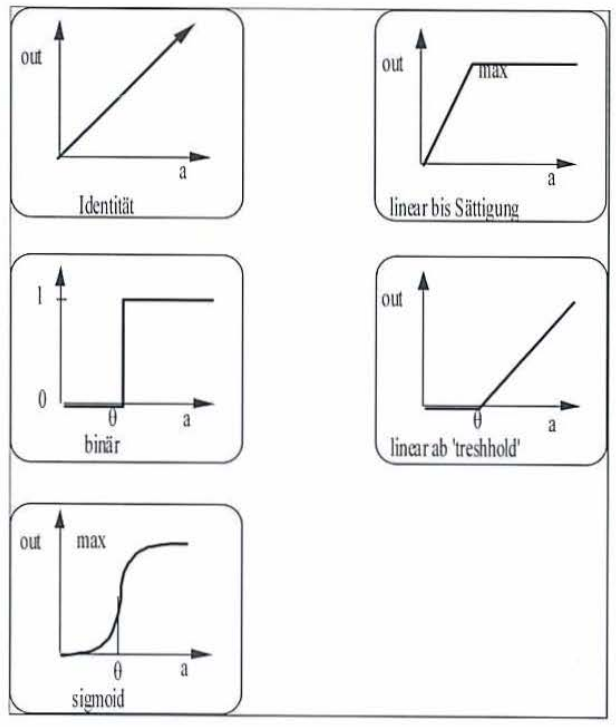
\includegraphics[width=\linewidth]{figures/ch01_Ausgabefunktion.png}
	\caption{Häufig verwendete Ausgabefunktionen}
	\label{fig:ausgabefunktionen}
\end{figure}

\subsection{Verbindungsnetzwerke}
Üblicherweise wird das Verbindungsnetzwerk der Zellen in
einer Matrixschreibweise angegeben: $w_{ij}$ ist eine Verbindung von Zelle $i$ nach Zelle $j$. Für die Verbindungsmatrix $\textbf{W} = [w_{ij}]$ gilt dann: ein Eintrag in der Matrix $\textbf{W}$ mit
\begin{itemize}
\item $w_{ij} = 0$ gibt an, daß keine Verbindung zwischen $i$ und $j$ existiert,
\item $w_{ij} < 0$ gibt an, daß Neuron $i$ seinen Nachfolger $j$ durch ein Gewicht der
Stärke $|w_{ij}|$ hemmt,
\item $w_{ij} > 0$ gibt an, daß Neuron $i$ seinen Nachfolger $j$ durch ein Gewicht der
Stärke $|w_{ij}|$ anregt.
\end{itemize}
%In der Implementierung in einem Software-Simulator wird häufig eine Speicherung der Verbindungsgewichte gewählt, bei der nur tatsächlich vorhandene Gewichte Speicherplatz benötigen, z.B. eine Zeigerstruktur, bei der jedes Neuron eine verkettete Liste aller Eingangsgewichte besitzt, von denen jedes wiederum einen Zeiger auf das Neuron besitzt, von dem die Verbindung ausgeht. Diese Art der Implementierung über sogenannte rückwärtsgerichtete Adjazenzlisten hat sich auf Workstations weitgehend durchgesetzt. Bei einer Realisierung als Matrix benötigt ein Netz mit n Neuronen nämlich immer Speicherplatz der Größe n^2 . Dies ist besonders für feedforward-Netze mit mehreren Ebenen eine große Verschwendung. 

Folgende Topologien neuronaler Netze kommen besonders häufig in Simulationen vor:
\begin{itemize}
\item \textbf{feedforward-Netze:} enthalten keine Zyklen
\item \textbf{feedback-Netze:} enthalten Zyklen (feedback)
\item \textbf{hierarchische Netze:} Gliederung in mehrere Ebenen
\end{itemize}

\subsection{Propagierungsregel}
gibt die Gesamteingabe aller Nachbarzellen an und hat bei sehr vielen Modellen die Form:\\
$net_j(t) = \sum_i o_i(t)w_{ij} = O(t)W_j$ (gewichtete Summe)\\
Dabei ist $O(t) = (o_1(t),...,o_n(t))$ ein Zeilenvektor, $W_j$ die $j$-te Spalte der Gewichtsmatrix $\textbf{W}$:\\
$Net(t) = O(t)W =  (o_1(t),...,o_n(t))\begin{pmatrix}
w_{11} & ... & w_{1m}\\
w_{n1} & ... & w_{nm}\\
\end{pmatrix}$ \newline
Biologisch motiviert kann man auch die anregenden (exzitatorischen) und hemmenden (inhibitorischen) Verbindungen in zwei verschiedene Gewichtsmatrizen mit nur positiven Gewichten speichern: \\
\begin{align*}
net_j(t) &= net_{excit,j} - net_{inhib,j}\\
net_{excit,j} &= \sum_i o_i(t)w_{excit,ij}\\
net_{inhib,j} &= \sum_i o_i(t)w_{inhib,ij} \text{ bzw. }\\
Net(t) &= O(t)W_{excit} - O(t)W_{inhib}
\end{align*}

\subsection{Aktivierungsfunktion}
Berechnet einen Aktivierungszustand aus altem Zustand und Eingabewerten\\
$a_i(t+1) = f_{act}(a_i(t), net_i(t), \theta_i)$
\begin{itemize}
\item deterministische Aktivierungsfunktion $f$: Ergebnis eindeutig durch die Eingabe bestimmt
\item stochastische Aktivierungsfunktion $f$: Ergebnis durch eine Zufallsverteilung abhängig von der Eingabe bestimmt
\end{itemize}

\subsection{Lernregel}

Theoretisch mögliche Arten des Lernens:
\begin{itemize}
\item[1.]Entwicklung neuer Verbindungen
\item[2.]Löschen existierender Verbindungen
\item[3.]Modifikation der Stärke $w_{ij}$ von Verbindungen
\item[4.]Entwicklung neuer Zellen
\end{itemize}
1. und 2. kann durch 3. approximiert werden:\\
Neue Verbindung: $w_{ij} = 0 \rightarrow w_{ij} \neq 0$\\
Löschen: $w_{ij} \neq 0 \rightarrow w_{ij} = 0$
Aktuelle Lernverfahren arbeiten meist nur durch Modifikation der Verbindungen.
Tabelle \ref{tab:lernregeln} zeigt wichtige Lernregeln.
\begin{table}
\centering
\begin{tabular}{|p{9cm}|}
	\hline
	\textbf{Hebb'sche Lernregel:}\newline Wenn Zelle $u_j$ Eingabe von $u_i$ erhält und beide geichzeitig stark aktiviert sind, soll Gewicht $w_{ij}$ (Bindungsstärke von $u_i$ nach $u_j$) erhöht werden: \newline $\delta w_{ij} = \eta o_ia_j$ \newline $\eta$ = Lernrate \newline
	allgemein: $\delta w_{ij} = h(o_i, w_{ij})\cdot g(a_j, t_j)$, \newline
	$t_i$ = erwartete Aktivierung (\glqq teaching input\grqq)\\
	\hline
	\textbf{Delta-Regel (Widrow-Hoff-Regel):}\newline
	$\delta w_{ij} = \eta o_i(t_j - a_j) = \eta o_i \delta_j$ \newline Gewichtsänderung propotional zur Differenz $\delta$  der Aktivierung und der erwarteten Aktivierung, verallgem. Lernregel für Perzeptrons\\
	\hline
	\textbf{Grossberg's Regel:} \newline
	$\delta w_{ij} = \eta (o_i - w_{ij})a_j$ \newline
	Änderung propotional zur Differenz zwischen Ausgabe und Gewicht der Vorgängerzelle\\
	\hline
	\textbf{Backpropagation (verallgem. Delta-Regel):}
	siehe nächstes Kapitel\\
	\hline
\end{tabular}
\caption{Wichtige Lernregeln}
\label{tab:lernregeln}
\end{table}

\section*{Komponenten neuronaler Modelle}
% K
% Was es so für neuronale Modelle gibt
Ausgangsfrage: \textbf{Wann} werden die Aktivierungen der Zellen neu berechnet?\\
\begin{itemize}
\item \textbf{Asynchrone Modelle:} Einzelne Zellen ändern ihre Werte zu verschiedenen Zeitpunkten
\begin{itemize}
\item[1.] \textbf{Feste Ordnung:} Jede Zelle $u_i$ berechnet neue Aktivierung $a_i$ und Ausgabe $o_i$ bevor nächste Zelle besucht wird
\item[2.] \textbf{Zufällige Auswahl:} Wähle zufällig eine Zelle $u_i$, berechne $a_i$ und $o_i$; wiederhole dies bis zum Ende
\end{itemize}
\item \textbf{Synchrone Modelle:} alle Zellen ändern ihre Werte leichzeitig. Berechne neue Aktivierung aller Zellen (quasi-) gleichzeitig; berechne erst danach neue Ausgabewerte aller Zellen 
\end{itemize}

\subsection{Aktivierungsfunktionen}
Bermerkung: Häufig werden (wie im Folgenden) Aktivierungsfunktion $f_{act}$ und Ausgabefunktion $f_{out}$ zu einer Funktion $f$ zusammengefasst und dann wieder als Aktivierungsfunktion bezeichnet.\\
\subsubsection*{Lineare Aktivierungsfunktionen}
Hierbei können alle Netzwerke mit mehreren ebenen durch ein Netzwerk mit nur Input- und Output-Ebene mit andereren gewichten realisiert werden!

\subsubsection*{Schrittfunktion}
$o_j = \begin{cases} 1 & net_j \geq \theta_j\\ 0 & sonst \end{cases}$

%------------------------------------------------
\section{Perzeptron}
%Kap. 7 bei Zell
% -----------------------------------------------------------------------
% -----------------------------------------------------------------------
\section*{Aufbau}
% Zell: Kapitel 7.1
Es gibt eigentlich historisch gesehen nicht \textit{das} Perzeptron, sondern eine ganze Familie verwandter Modelle neuronaler Netze, die von Frank Rosenblatt Anfang der 60er Jahre entwickelt wurden und die alle mit Perzeptron bezeichnet wurden.

Ein allgemeines Perzeptron hat folgenden Aufbau (Vgl. Abbildung \ref{fig:perzeptron-minsky-papert}):
\begin{itemize}
	\item \emph{Schicht mit Eingabezellen} \\
	Retina - Dient der reinen Datenaufnahme (Muster) und hat festgewichtete Verbindungen zur nächsten Neuronenschicht. (Diese Schicht wird im Folgenden oftmals nicht dargestellt.)
	
	\item \emph{Schicht mit Neuronen} \\
	Eingabeschicht - Neuronen ohne Informationsverarbeitung jedoch mit trainierbaren Verbindungen zum Ausgabeneuron.

	\item Ausgabeneuron $\Omega$ \\
	Klassifikator - Neuron mit Informationsverarbeitung, welches angibt, ob das an der Retina anliegende Muster vom Perzeptron erkannt wird oder nicht.
\end{itemize}

\begin{figure}[ht!] \centering 
	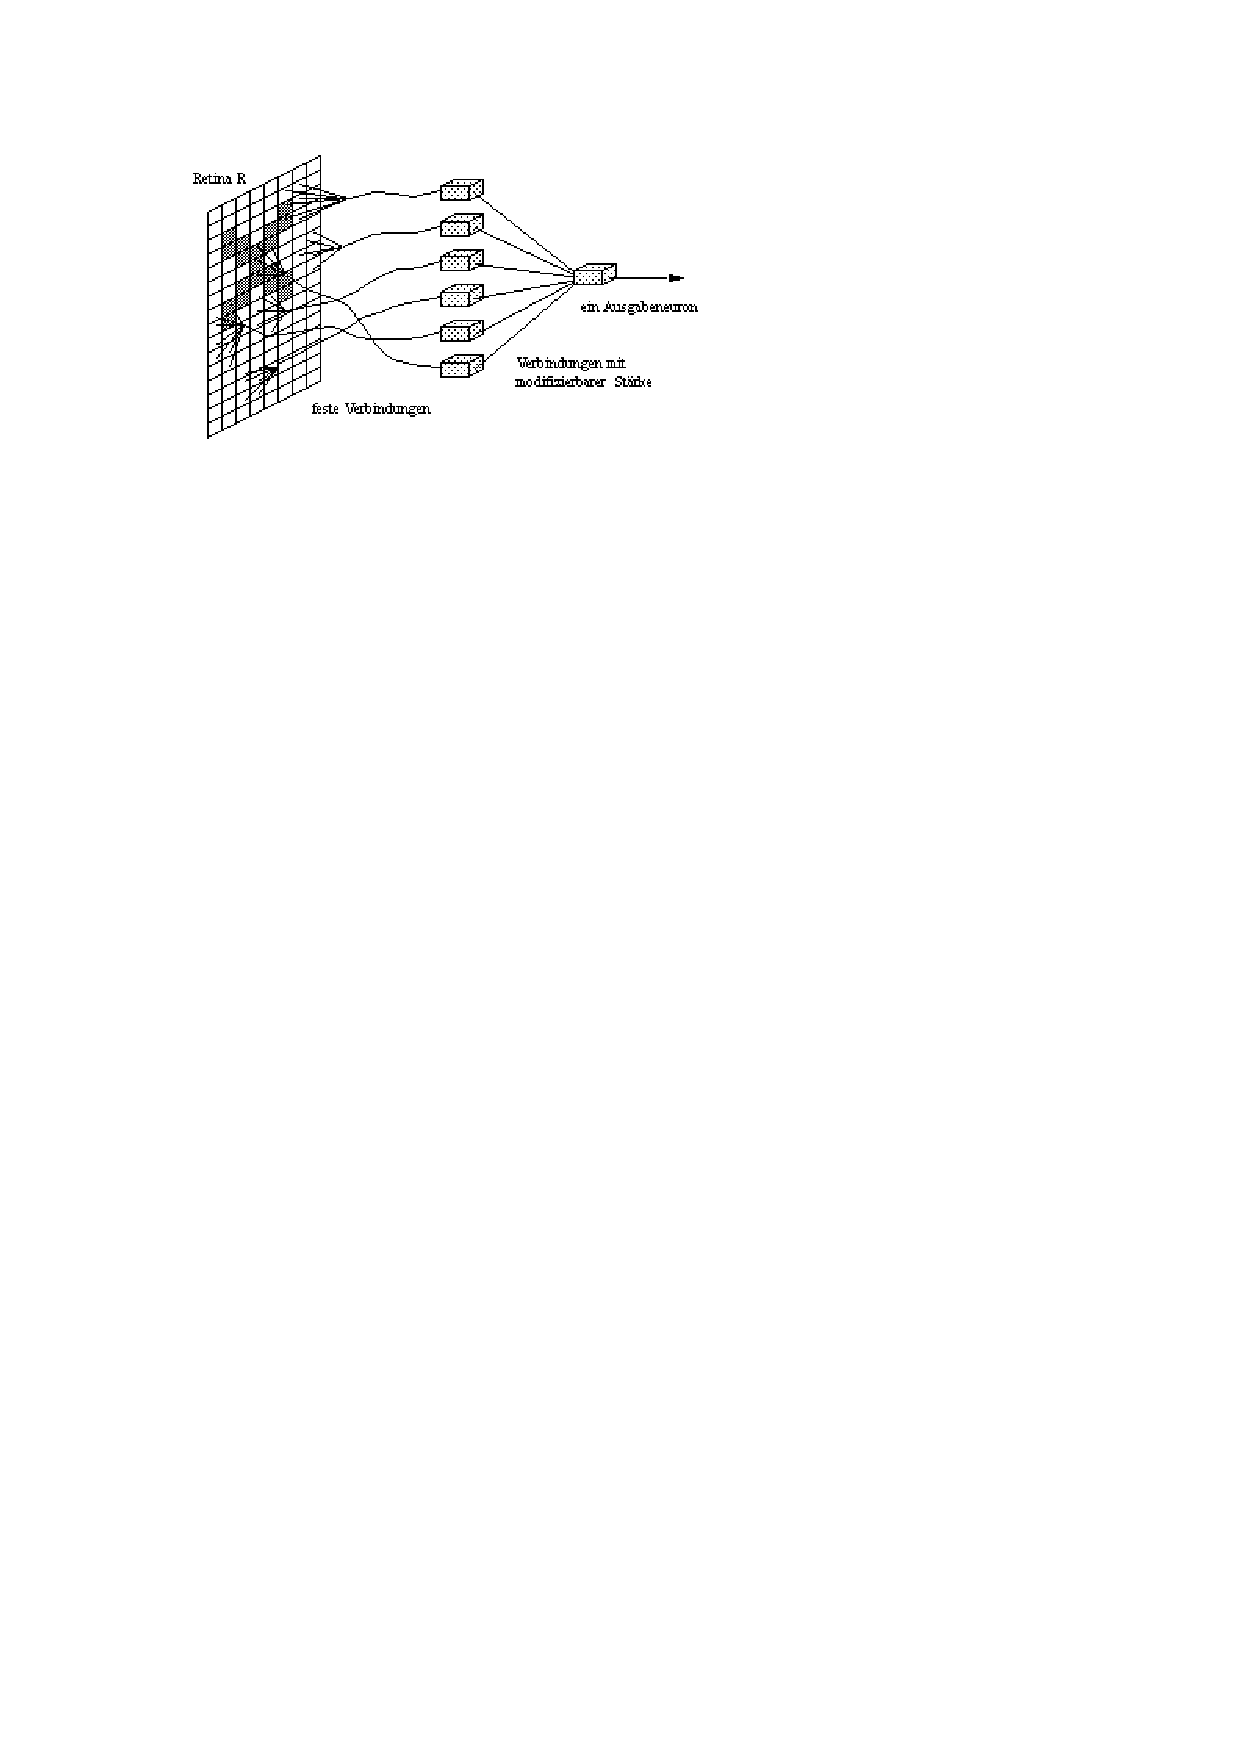
\includegraphics[width=\linewidth]{figures/ch02_perzeptron-minsky-papert.pdf}
	\caption{Struktur des Perzeptron nach Minsky und Papert.}
	\label{fig:perzeptron-minsky-papert}
\end{figure}

Weiterhin wird unter dem Begriff \emph{Perzeptron} oft das binäre Modell des Perzeptrons verstanden, bei dem die Eingaben und die Aktivierungen der Neuronen nur binäre Werte 0 und 1 (bzw. -1 und 1) annehmen dürfen. Die Gewichte können allerdings beliebige reelle Werte annehmen.

% -----------------------------------------------------------------------
\subsection*{Neuronen des Perzeptrons}
% Zell: Kapitel 7.2
Die Neuronen der Eingabeschicht werden in diesem Modell nicht spezifiziert. Es genügt, wenn man sie als \emph{binäre Eingaben} betrachtet.
Damit kann das Schema eines Perzeptrons wie in Abbildung \ref{fig:perzeptron-schema} links dargestellt werden. Dabei ist jedes Neuron der Ebene 0 fest mit allen Neuronen der Eingabeschicht verbunden.

\begin{figure}[ht!] \centering 
	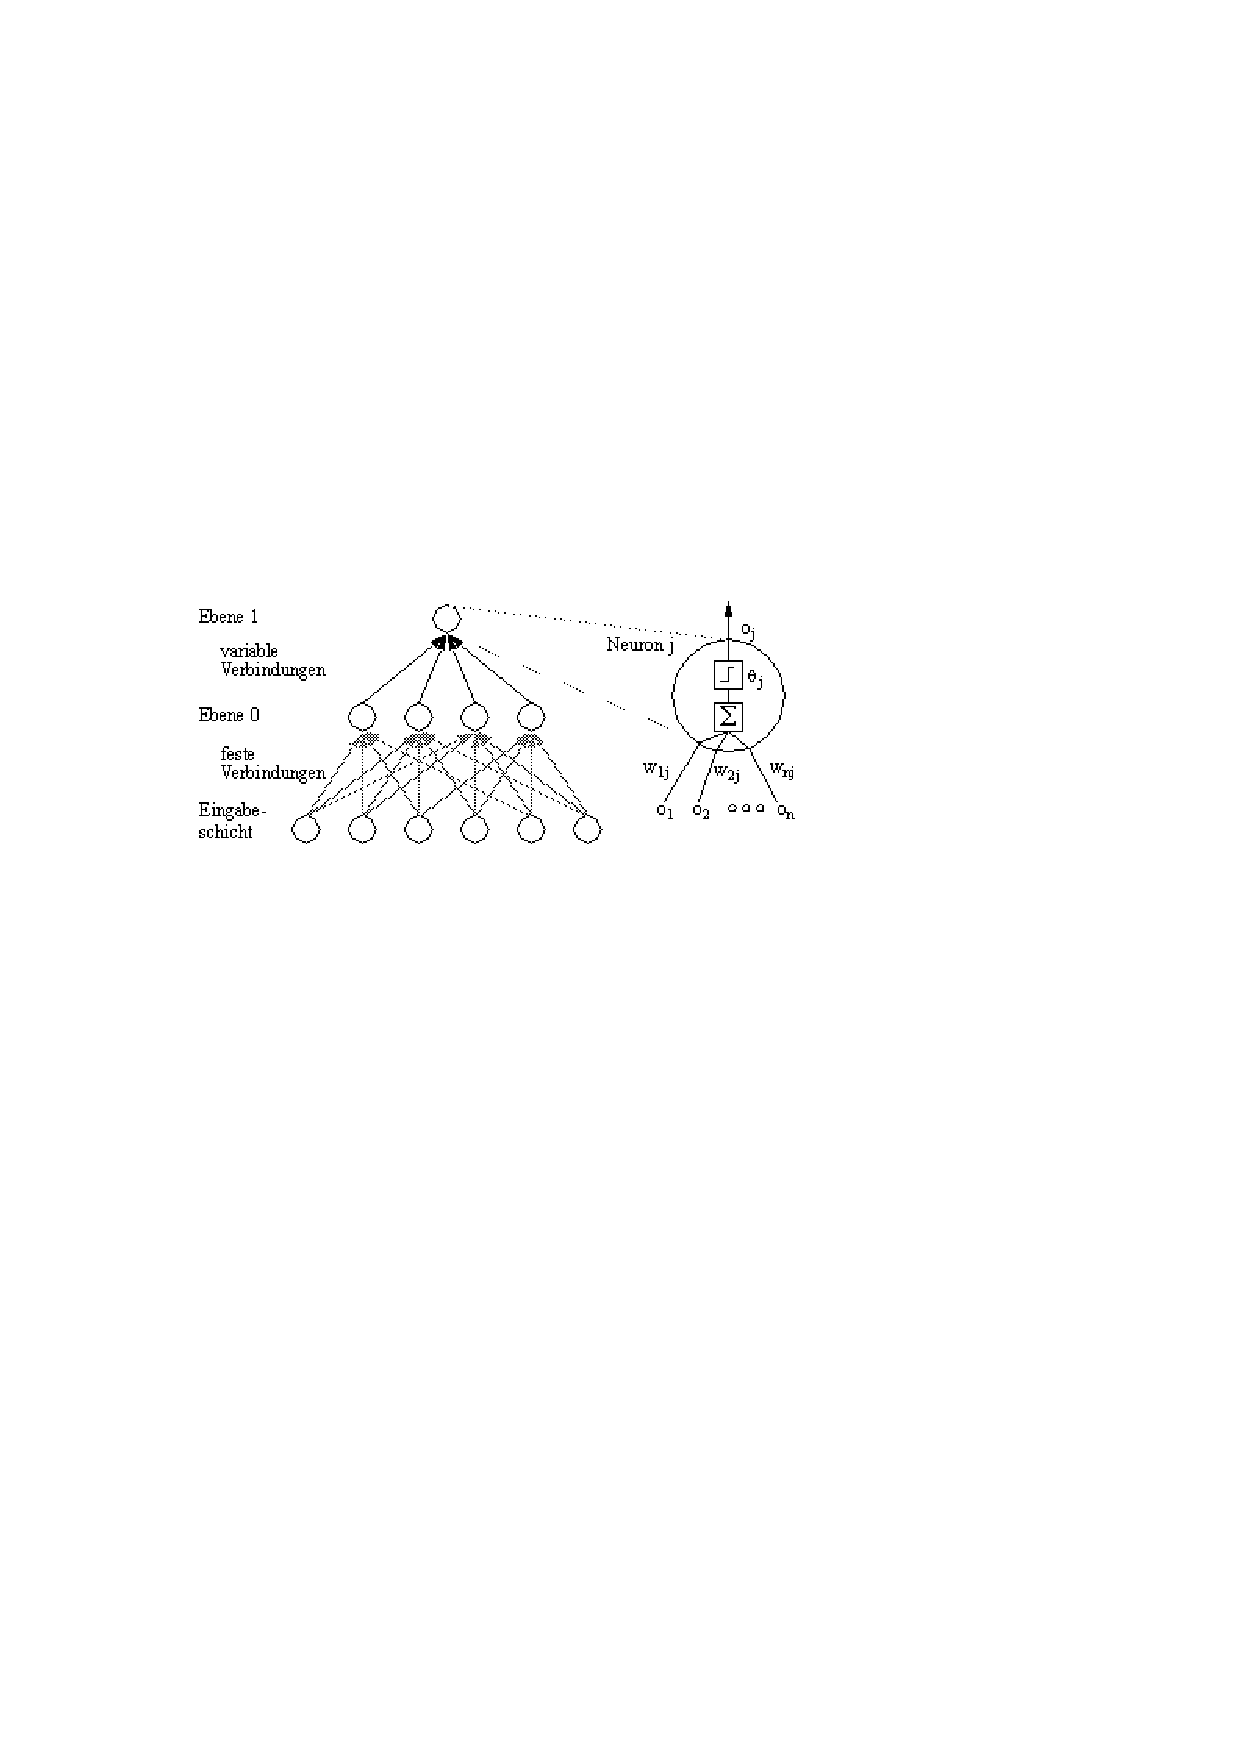
\includegraphics[width=\linewidth]{figures/ch02_perzeptron-schema.pdf}
	\caption{Schema des Perzeptrons (links) und Ausgabeneuron des Perzeptrons (rechts).}
	\label{fig:perzeptron-schema}
\end{figure}

Jedes Neuron der Ebenen 0 und 1 des Perzeptrons hat das in Abbildung \ref{fig:perzeptron-schema} rechts dargestellte Verhalten: Es summiert seine Eingaben auf ($net_j$), die sich als Ausgaben der Vorgängerneuronen ($o_i$) multipliziert mit dem jeweiligen Gewicht $w_{ij}$ ergeben: 
\[
	net_j = \sum_i o_i \cdot w_{ij}
\]

 Auf diese Netzeingabe $net_j$ wird eine binäre Schwellenwertfuktion angewandt: Die Ausgabe $o_j$ ist 1, falls die Netzeingabe größer oder gleich dem Schwellenwert $\theta_j$ ist, andernfalls ist die Ausgabe 0:
\[
	o_j = a_j = 
	\begin{cases}
		1 &\text{falls } net_j \ge \theta_j \\
		0 &\text{sonst}
	\end{cases}
\]

% -----------------------------------------------------------------------
\subsection*{Repräsentierbarkeit und Lernfähigkeit}

\subsubsection*{Repräsentierbarkeit} 
Repräsentierbarkeit bezeichnet die Fähigkeit eines Netzes, eine gegebene Funktion (Prädikat) mit dem neuronalen Netz realisieren zu können. Hierbei ist die Topologie des Netzes vorgegeben, es dürfen aber alle Gewichte und Schwellenwerte korrekt bzw. optimal gewählt werden.

\subsubsection*{Lernfähigkeit} 
Lernfähigkeit ist die Fähigkeit eines Lernalgorithmus, ein Netzwerk eine repräsentierbare Funktion (Prädikat) lernen zu lassen. D.h. die Gewichte und Schwellenwerte durch den \emph{Algorithmus} korrekt zu bestimmen. \\

Die Unterscheidung zwischen Repräsentierbarkeit und Lernfähigkeit ist sehr wichtig\footnote{Die Unterscheidung ist auch aus historischen Gründen sehr wichtig, weil sie in der ersten Blütephase neuronaler Netze noch nicht bekannt war und daher ein berühmtes Theorem, das Perzeptron-Lern-Theorem von F. Rosenblatt über die Fähigkeit des Perzeptron-Lernalgorithmus, meist falsch verstanden wurde.}:
\emph{Repräsentierbarkeit} stellt eine Fähigkeit des Netzes dar und ist nur von der Topologie und den gewählten Aktivierungs- und Ausgabefunktionen des Netzes abhängig, jedoch unabhängig von einem gewählten Lernalgorithmus.
\emph{Lernfähigkeit} hingegen ist eine Eigenschaft eines speziellen Lernalgorithmus. 



% -----------------------------------------------------------------------
% -----------------------------------------------------------------------
\section*{Lineare Trennbarkeit}
% Zell: Kapitel 7.3
Das Konzept der linearen Trennbarkeit kann man am besten an einem einfachen Beispiel, dem bekannten XOR-Problem, demonstrieren. Man betrachte hierzu ein einstufiges Perzeptron-Netzwerk mit einem Ausgabeneuron $j$ in Ebene 1 und zwei Neuronen in Ebene 0. Die Ausgabe des Neurons $j$ soll 0 sein, falls seine binären Eingaben gleich sind ($o_1 = o_2$) sonst soll sie 1 sein. Das heißt, damit $o_j = 1$ ist, muss gelten:
\[
	net_j = o_1 w_{1j} + o_2 w_{2j} \ge \theta_j
\]
Für $w_{2j} \ge 0$ ist dies äquivalent zu der Ungleichung
\[
	o_2 \ge \frac{1}{w_{2j}} ( \theta_j - o_1 w_{1j})
\]
Für einen konstanten Schwellwert $\theta_j$ ergibt sich also eine Gerade in der durch $o_1$ und $o_2$ gebildeten Ebene (siehe Abbildung \ref{fig:lineare-separierbarkeit}). Alle Punkte oberhalb dieser Geraden stellen bei positivem $w_{2j}$ Kombinationen von $o_1$ und $o_2$ dar, für die das Neuron feuert. Bei negativem $w_{2j}$ sind alle Punkte unterhalb der Geraden Punkte, für die das Neuron feuert.

\begin{figure}[ht!] \centering 
	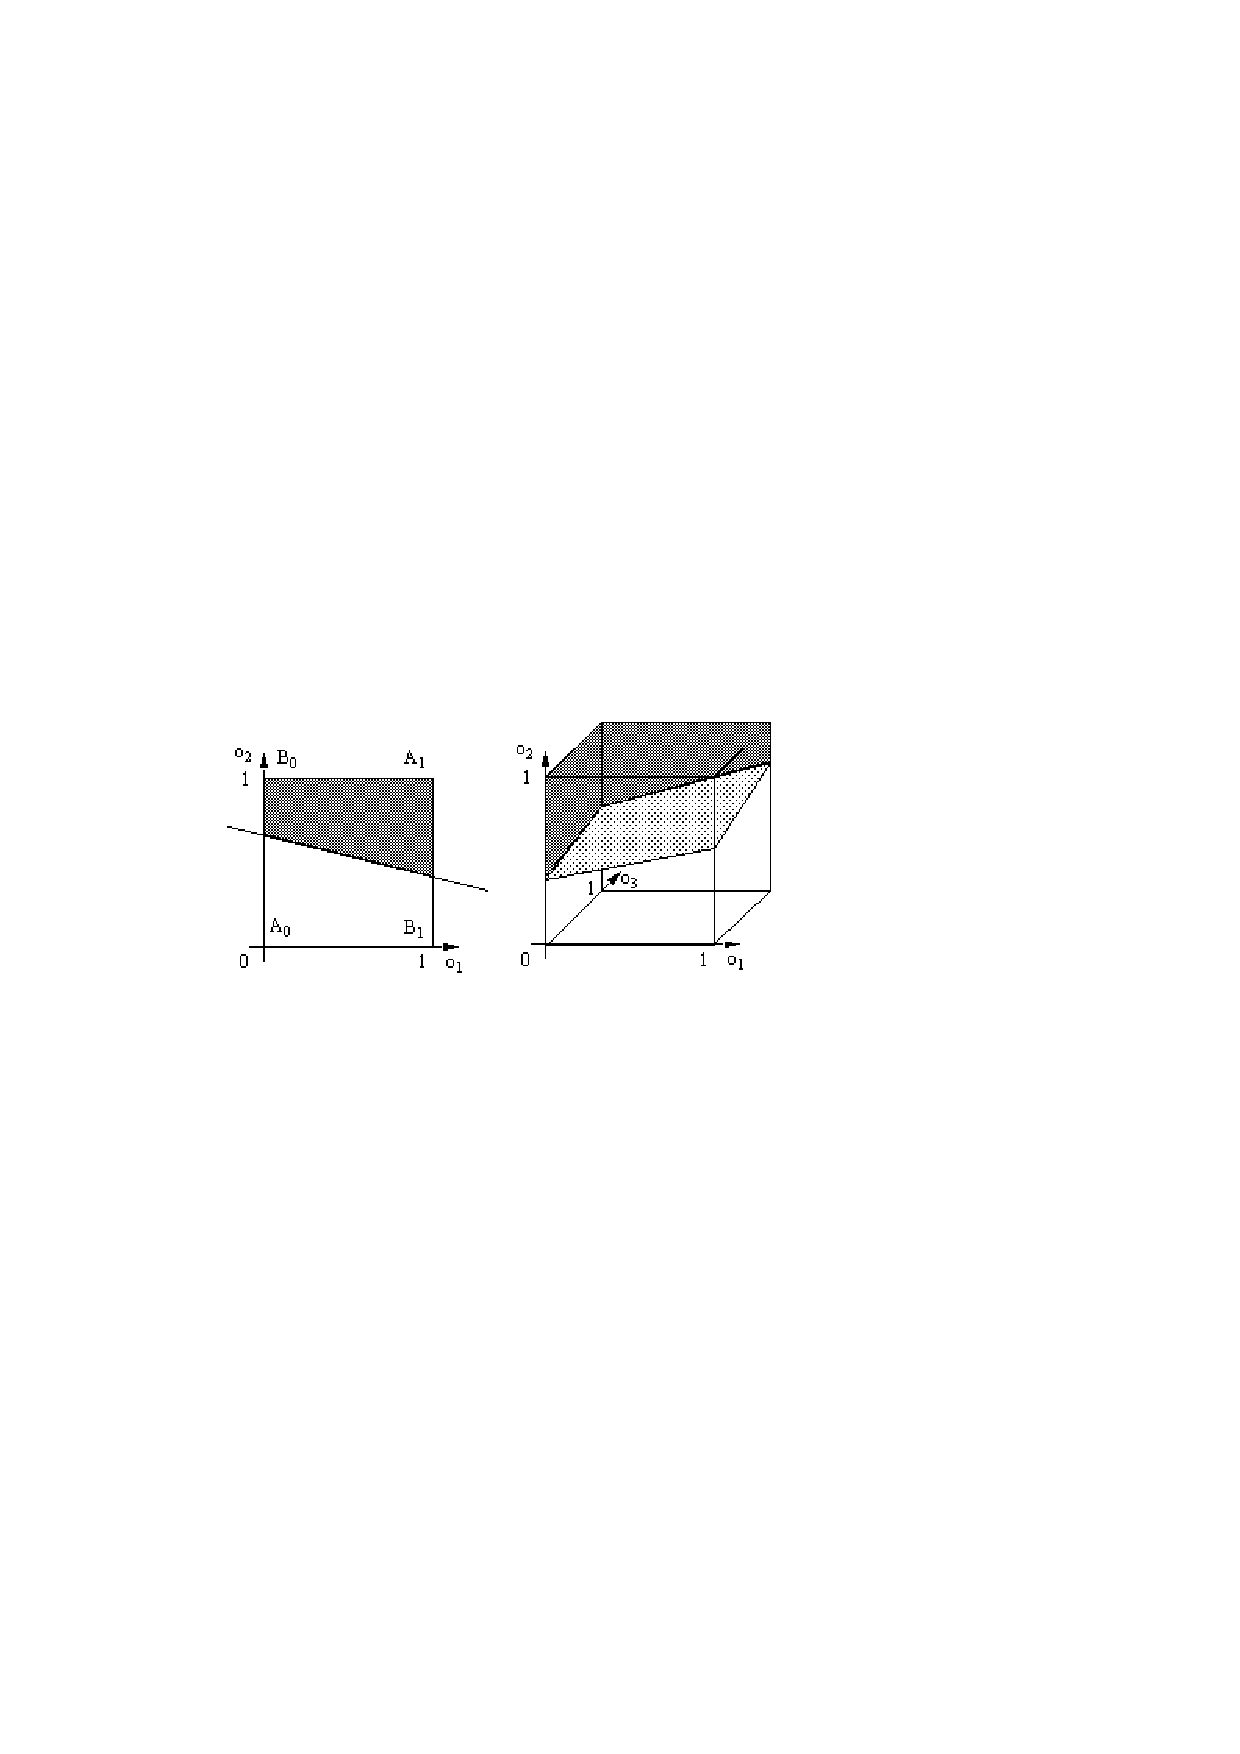
\includegraphics[width=\linewidth]{figures/ch02_lineare-trennbarkeit.pdf}
	\caption{Lineare Trennbarkeit und das XOR-Problem.}
	\label{fig:lineare-separierbarkeit}
\end{figure}

Ein neuronales Netz, welches das XOR-Problem lösen will, muss die Punkte $A_0 (0|0)$ und $A_1 (1|1)$ einer Klasse A zuordnen, die Punkte $B_0 (0|1)$ und $B_1 (1|0)$ der Klasse B. Diese Trennung ist mit einer einzigen Gerade, welche den Eingabereaum linear trennt, nicht möglich. 
Deshalb gilt: Die Menge $A = \{A_0, A_1\}$ und $B = \{B_0, B_1\}$ des XOR-Problems sind nicht linear separierbar, d.h. es gibt keine Wertekombination von $w_{1j}$, $w_{2j}$ und $\theta_j$, für die $net_j < \theta_j$ für alle Punkte in A und zugleich $net_j \ge \theta_j$ für alle Punkte in B ist.

Bei $n$ Eingängen eines Neurons, kann man den Raum der Eingaben als n-dimensionalen Würfel darstellen (sofern die Eingaben auf $[0,1]$ beschränkt ist, sonst ist es der n-dimensionale Raum).
Das Neuron trennt diesen Eingaberaum durch eine $(n-1)$-dimensionale \emph{Hyperebene}. Für $n=3$ ist dies in Abbildung \ref{fig:lineare-separierbarkeit} dargestellt.

Allgemein gilt: Ein einstufiges Perzeptron (d.h. ein Perzeptron mit nur einer Stufe modifizierbarer Gewichte) kann nur linear separierbare Mengen, d.h. Mengen, die durch eine Hyperebene trennbar sind, klassifizieren.


% -----------------------------------------------------------------------
\subsection*{Entscheidungsfunktion $g(x)$}
Eine Entscheidungsfunktion weißt einem Eingabevektor $\vec{x}$ eine der $k$ Klassen zu. Diese Klasse wird als $C_k$ bezeichnet.
Es seien folgende Werte gegeben:
\begin{align*}
	& \vec{x} = (x_1, \ldots, x_n)^T &\text{Merkmalsvektor} \\
	& \vec{w} = (w_1, \ldots, w_n)^T &\text{Gewichtsvektor} \\
	& w_0	&\text{Bias/Threshold}
\end{align*}

\subsubsection*{Zwei Klassen}
Bei $k=2$ gilt die einfachste Form der Entscheidungsfunktion $g(x)$:
\[
	g(\vec{x}) = \sum_{i=1}^{n} w_i x_i + w_0 = \vec{w}^T \vec{x} + w_0
\]
Der Merkmalsvektor $\vec{x}$ wird der Klasse $C_1$ zugeordnet wenn $g(\vec{x}) \ge 0$, andernfalls wird er der Klasse $C_2$ zugeordnet. Die Entscheidungsfunktion $g(x)$ gibt den Abstand zwischen Entscheidungsgrenze und Merkmalsvektor zurück. 

Die Entscheidungsgrenze ist damit für $g(\vec{x}) = 0$ definiert. Sie entspricht einer $(d-1)$-dimensionalen Hyperebene innerhalb eines $d$-dimensionalen Merkmalsraums und wird mit $H$ bezeichnet:
\[
	H: g(\vec{x}) = \sum_{i=1}^{n} w_i x_i + w_0 = \vec{w}^T \vec{x} + w_0 = 0
\]
Der normierte Vektor $\vec{w}$ gibt die Richtung und der Bias $w_0$ die Lage dieser Entscheidungsgrenze an. Die Hyperebene $H$ trennt den Merkmalsraum in zwei Hälften auf; Entscheidungsregion $R_1$ für $C_1$ und $R_2$ für $C_2$. Liegt $\vec{x}$ in $R_1$ ($g(x) \ge 0$), zeigt auch der Normalenvektor $\vec{w}$ in $R_1$. Abbildung \ref{fig:lineare-entscheidunsfunktion} zeigt dies. Für den Abstand $r$ zwischen Hyperebene $H$ und Merkmalsvektor $\vec{x}$ gilt:
\[
	r = \frac{g(x)}{||w||}
\]

\begin{figure}[ht!] \centering 
	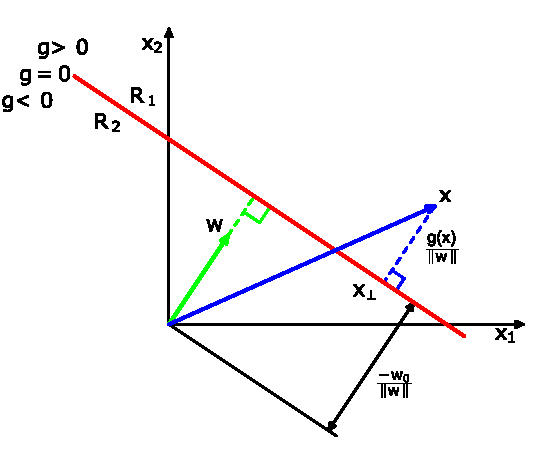
\includegraphics[width=\linewidth]{figures/ch02_lineare-entscheidungsfunktion.pdf}
	\caption{Grafisches Schaubild zur linearen Entscheidungsfunktion $g(x)$ in einem zweidimensionalen Merkmalsraum.}
	\label{fig:lineare-entscheidunsfunktion}
\end{figure}


\subsubsection*{Mehrere Klassen}
Bei $k > 2$ Klassen gibt es verschiedene Möglichkeiten eine k-Klassen-Diskriminantfunktion durch Kombinationen von Zwei-Klassen-Diskriminantfunktionen zu bestimmen:
\begin{itemize}
 	\item \emph{one-versus-the-rest} \\
 	$k-1$ Klassifikatoren die alle jeweils ein Zwei-Klassen-Problem lösen: Sie trennen Punkte, die zur Klasse $C_k$ gehören von Punkten, die nicht zu $C_k$ gehören (siehe Abbildung \ref{fig:lineare-entscheidungsfunktion-mehrere-klassen} oben).

 	\item \emph{one-versus-one} \\
 	Bei diesem Ansatz gibt es $\frac{k(k-1)}{2}$ binäre Diskriminantfunktionen: Eine für jedes mögliche Klassenpaar (siehe Abbildung \ref{fig:lineare-entscheidungsfunktion-mehrere-klassen} unten). 
 \end{itemize} 

\begin{figure}[ht!] \centering 
	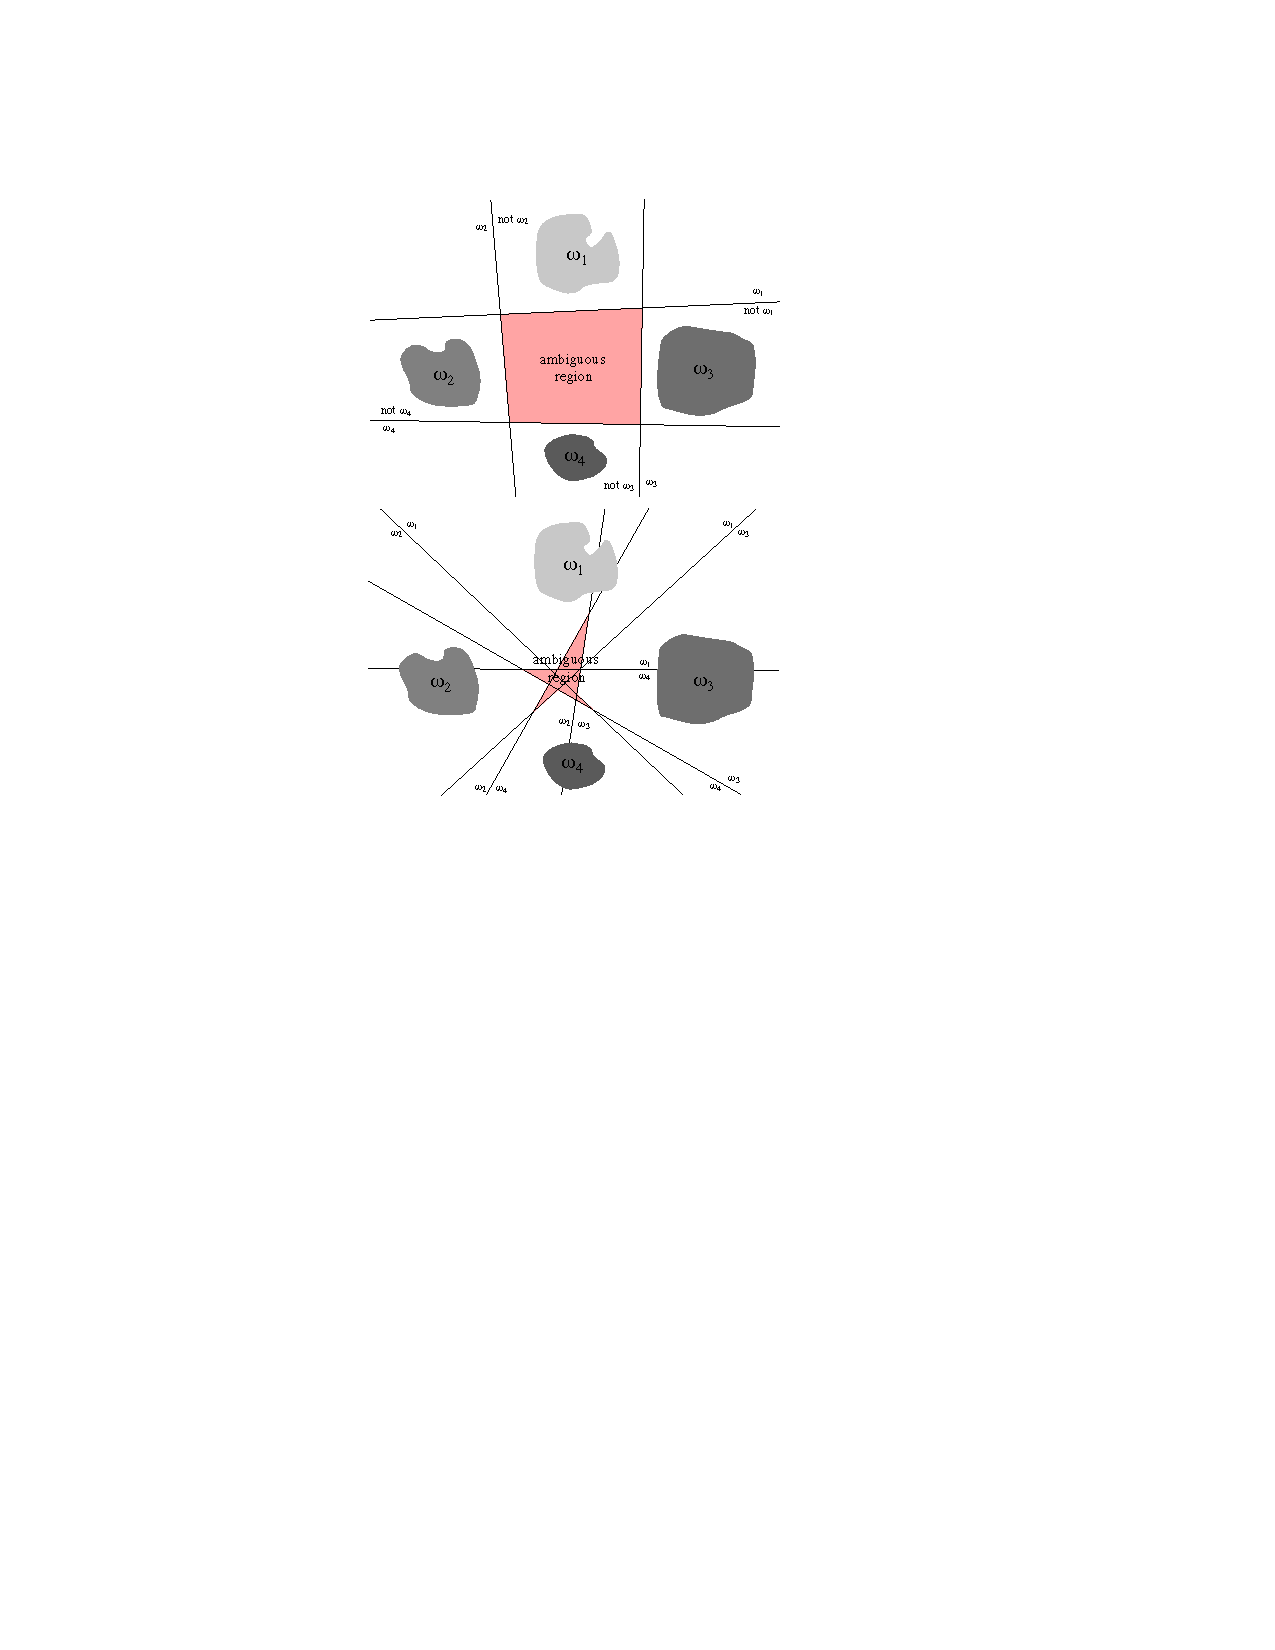
\includegraphics[width=\linewidth]{figures/ch02_lineare-entscheidungsfunktion-mehrere-klassen.pdf}
	\caption{Lineare Entscheidungsgrenzen für ein 4-Klassen-Problem. Oben der \emph{one-versus-the-rest} Ansatz ($C_i$ oder nicht $C_i$). Unten der \emph{one-versus-one} Ansatz ($C_i$ oder $C_j$ für alle $j \ne i$)}
	\label{fig:lineare-entscheidungsfunktion-mehrere-klassen}
\end{figure}

Beide Vorgehensweisen führen jedoch zu Bereichen des Merkmalsraums, welche nicht eindeutig einer Klasse zugeordnet werden können (in Abbildung \ref{fig:lineare-entscheidungsfunktion-mehrere-klassen} farbig hervorgehoben).
Deshalb wird für den Fall dass $k > 2$ ist der Ansatz der Entscheidungsfunktion für zwei Klassen wie folgt erweitert:
\[
	g_k(\vec{x}) = \vec{w}_k^T\vec{x} + w_{k0}
\]
Der daraus resultierende Klassifikator wird \emph{linear machine} genannt und teilt den Merkmalsraum in $k$ Entscheidungsregionen auf (siehe Abbildung \ref{fig:linear-machine}. Dabei ist $g_k(\vec{x})$ die größte Diskriminante, wenn $x$ in der Region $R_k$ liegt. Demnach wird der Merkmalsvektor $\vec{x}$ der Klasse $C_k$ zugeordnet, wenn gilt:
\[
	g_k(\vec{x}) > g_j(\vec{x}) \qquad \text{für alle } j \ne k
\]
Die Entscheidungsgrenze zwischen Klasse $C_k$ und Klasse $C_j$ ist gegeben für $g_k(\vec{x}) = g_j(\vec{x})$. Daraus folgt, analog zur Entscheidungsgrenze für den Zwei-Klassen-Fall, eine $(d-1)$-dimensionale Hyperebene, für die gilt:
\[
	(\vec{w}_k - \vec{w}_j)^T x + (w_{k0} - w_{j0}) = 0
\]
Im Gegensatz zur Entscheidungsgrenze im Zwei-Klassen-Fall ist hier nicht der Gewichtsvektor $\vec{w}$ entscheidend, sondern die Differenz $\vec{w}_k - \vec{w}_j$.

\begin{figure}[ht!] \centering 
	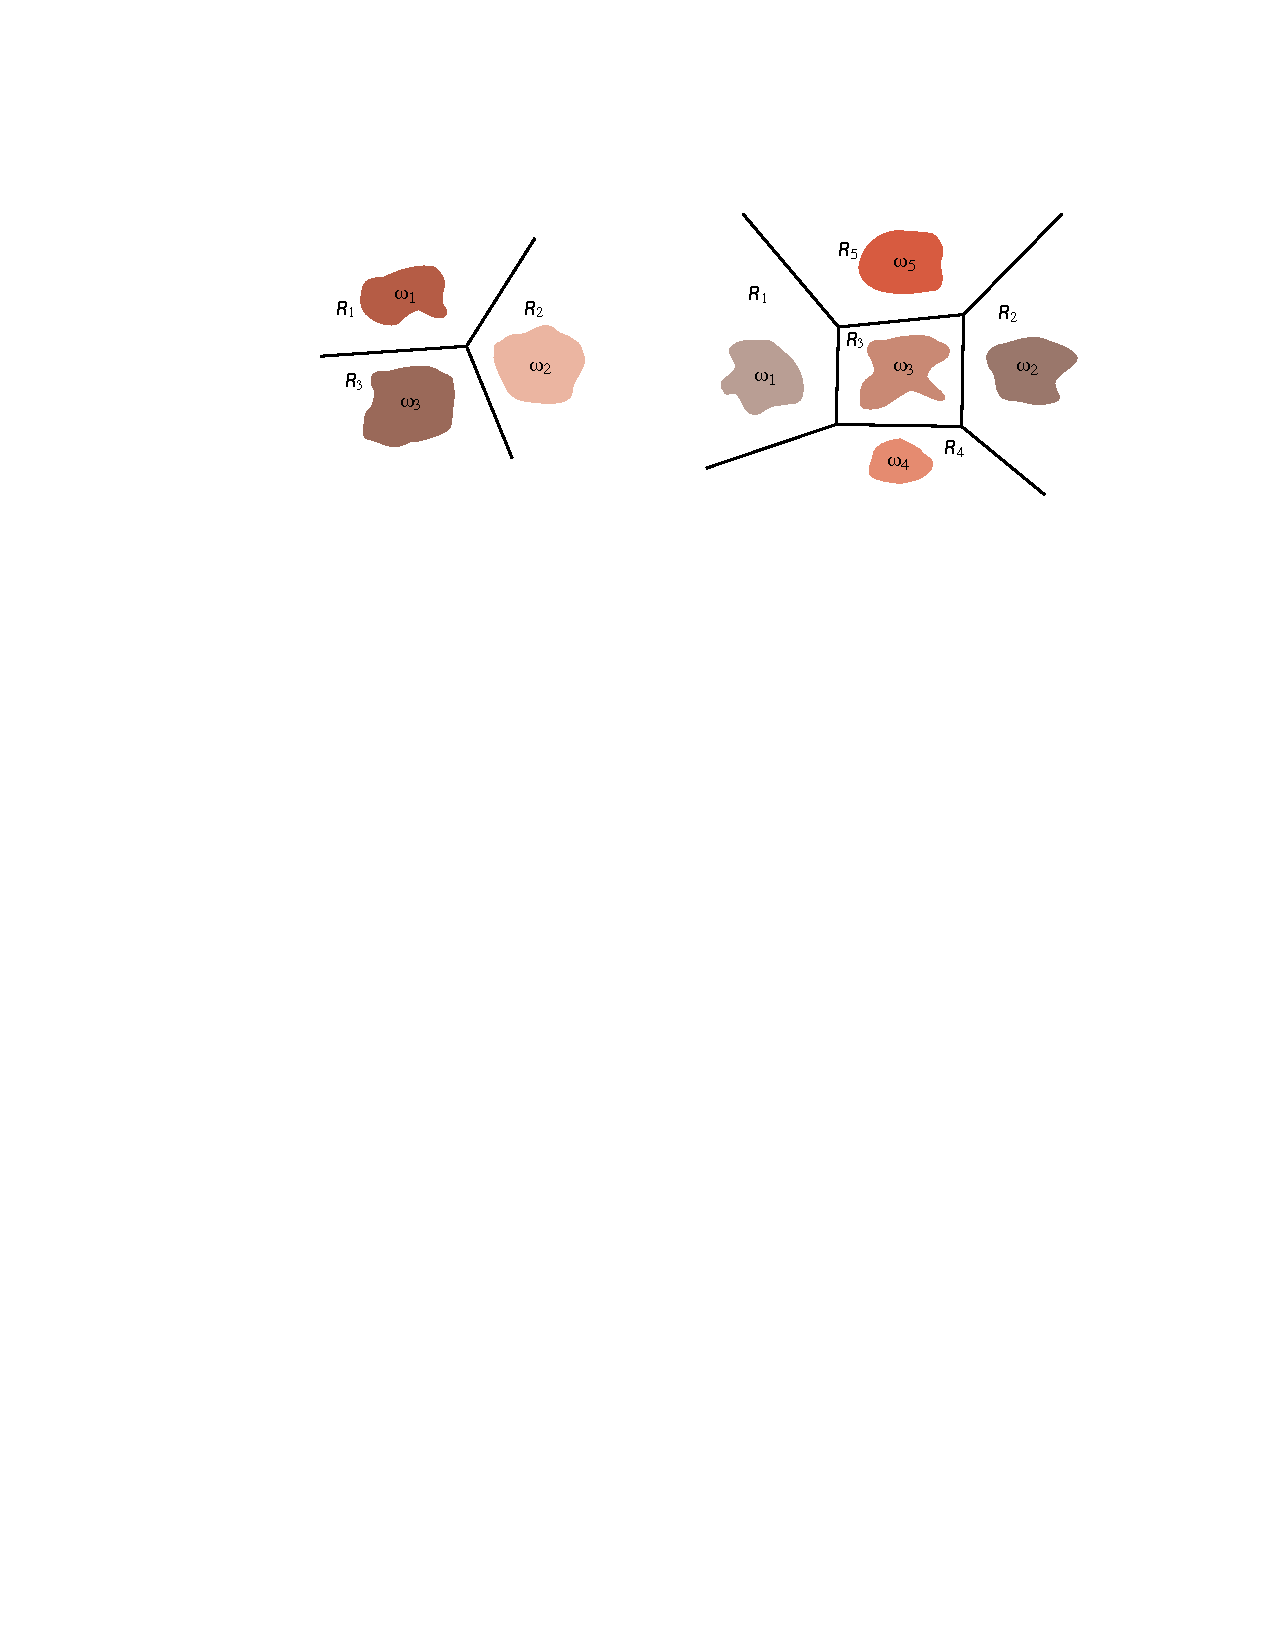
\includegraphics[width=\linewidth]{figures/ch02_linear-machine.pdf}
	\caption{Entscheidungsgrenzen erzeugt von einer \emph{linear machine} für ein Drei-Klassen- und ein Fünf-Klassen-Fall.}
	\label{fig:linear-machine}
\end{figure}


\subsubsection*{Least Squares}
ToDo

\subsubsection*{Fisher's linear discriminant}
ToDo


% -----------------------------------------------------------------------
% -----------------------------------------------------------------------
\section*{Multilayer-Perceptron (MLP)}
% -----------------------------------------------------------------------
\subsection*{Zweistufiges Perzeptron}
% Zell: Kapitel 7.4
Zweistufige binäre Perzeptrons sind mächtiger als einstufige, sie können konvexe Polygone klassifizieren. Dazu berechnen die Neuronen der ersten Ebene Hyperebenen wie im vorigen Fall auch, diese können dann aber in der zweiten Ebene durch ein Neuron, welches ein logisches AND durchführt, zum Schnitt gebracht werden, sodass sich ein konvexes Polygon ergibt.

Abbildung \ref{fig:perzeptron-zweistufig} zeigt ein Beispiel für ein zweistufiges Perzeptron und ein typisches Gebiet, dessen Punkte als Eingabe in das neuronale Netz aktzeptiert werden.

\begin{figure}[ht!] \centering 
	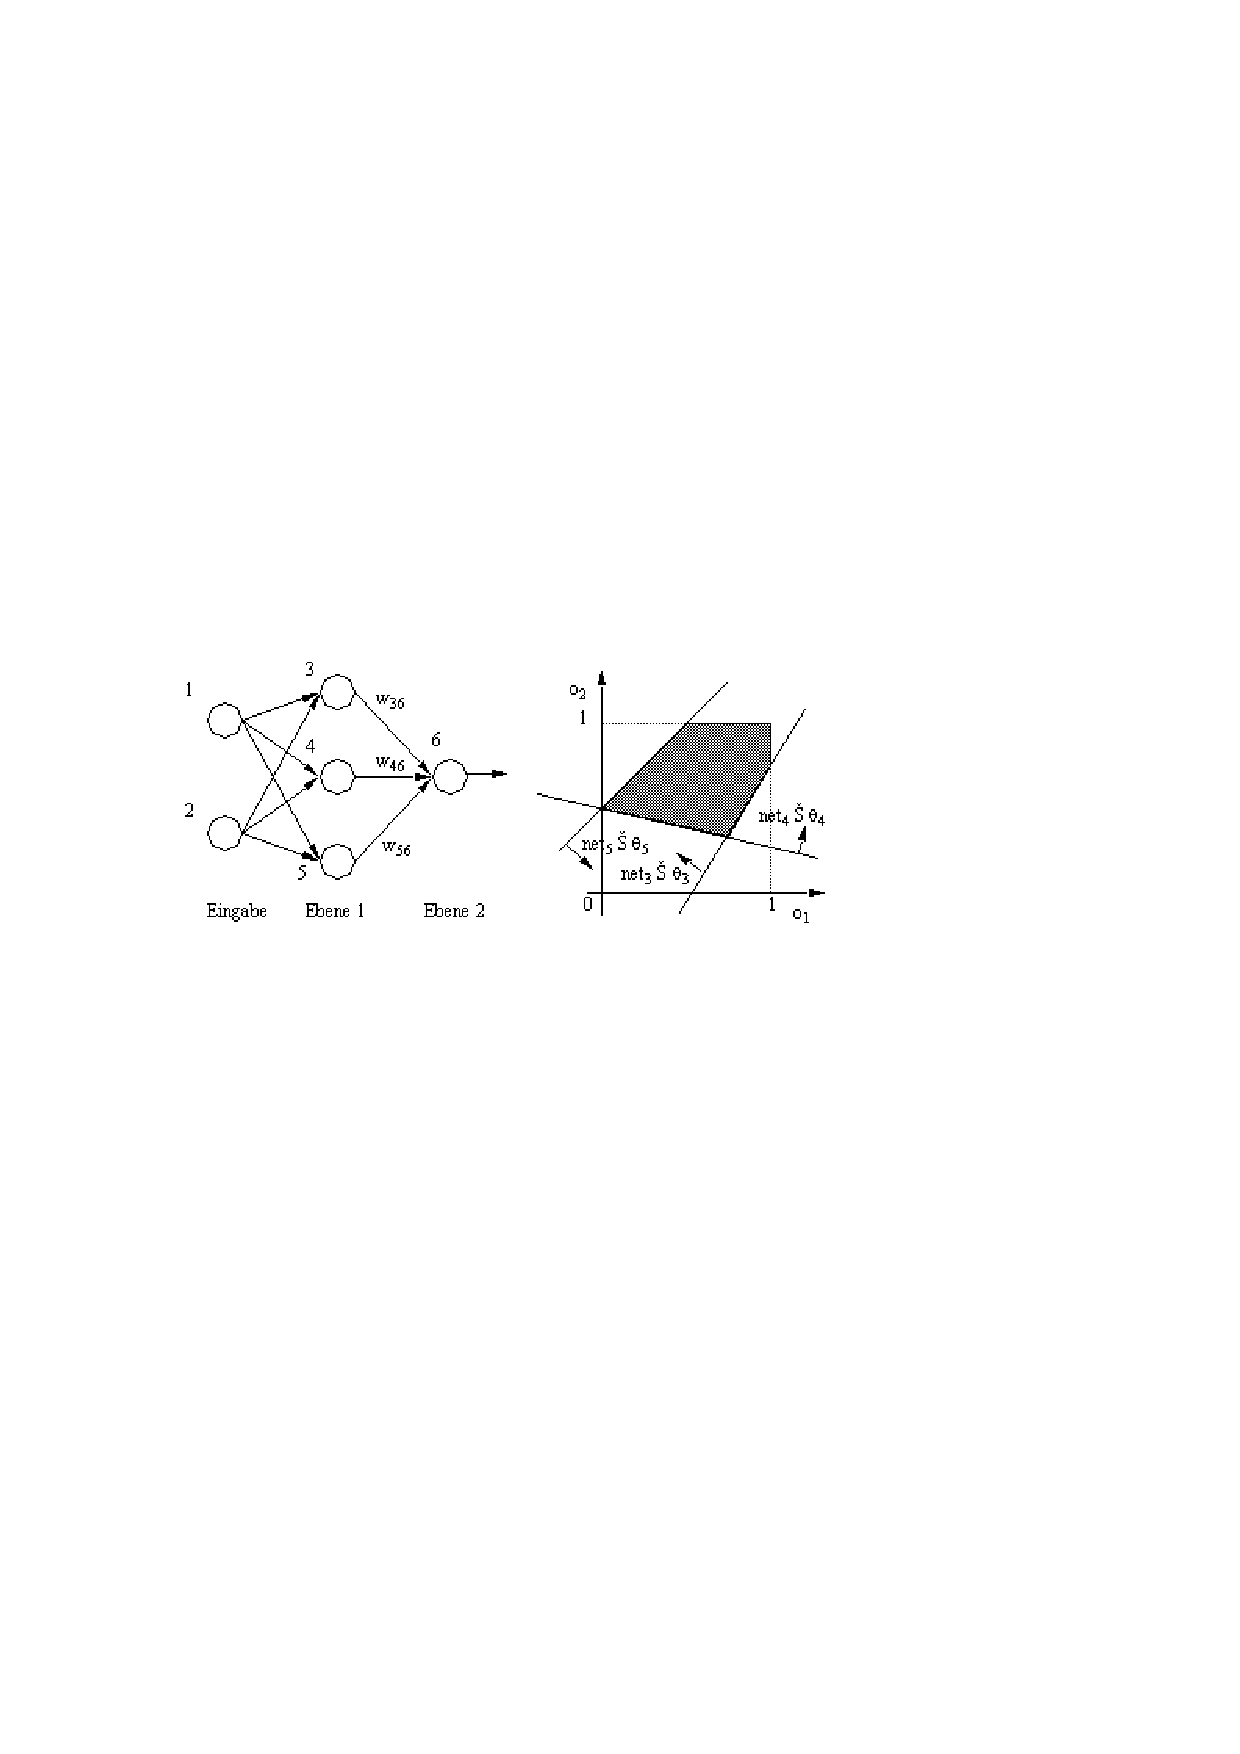
\includegraphics[width=\linewidth]{figures/ch02_perzeptron-zweistufig.pdf}
	\caption{Zweistufiges Perzeptron und ein von ihm akzeptiertes Gebiet im Merkmalsraum.}
	\label{fig:perzeptron-zweistufig}
\end{figure}

Die Funktion des logischen \emph{AND} kann dadurch erreicht werden, dass das Ausgangsneuron einen Schwellenwert besitzt, welcher der Summe der Gewichte der Verbindungen in dieses Neuron entspricht bzw. geringfügig kleiner ist:
Neuron 6 in Abbildung \ref{fig:perzeptron-zweistufig} führt durch $w_{36} = w_{46} = w_{56} = \frac{1}{3}$ und $\theta_6 = 0.9$ ein logisches AND\footnote{Die Verknüpfung der Gebiete ist nicht auf AND beschränkt. Sie könnte ebenfalls durch eine andere logische Funktion (z.B. OR, NAND, ...), welche sich mit einem einstufigen Perzeptron darstellen lässt, realisiert werden.} auf seine Eingabe durch. So wird $o_6 = 1$ genau dann, wenn $(o_1, o_2)$ im dunkel markierten konvexen Polygon liegt.

% -----------------------------------------------------------------------
\subsection*{Dreistufiges Perzeptron}
% Zell: Kapitel 7.5
Dreistufige binäre Perzeptrons können durch Überlagerung und Schnitt konvexer Polygone Mengen beliebiger Form repräsentieren. Abbildung \ref{fig:perzeptron-dreistufig} zeigt auch hierfür ein Beispiel.

\begin{figure}[ht!] \centering 
	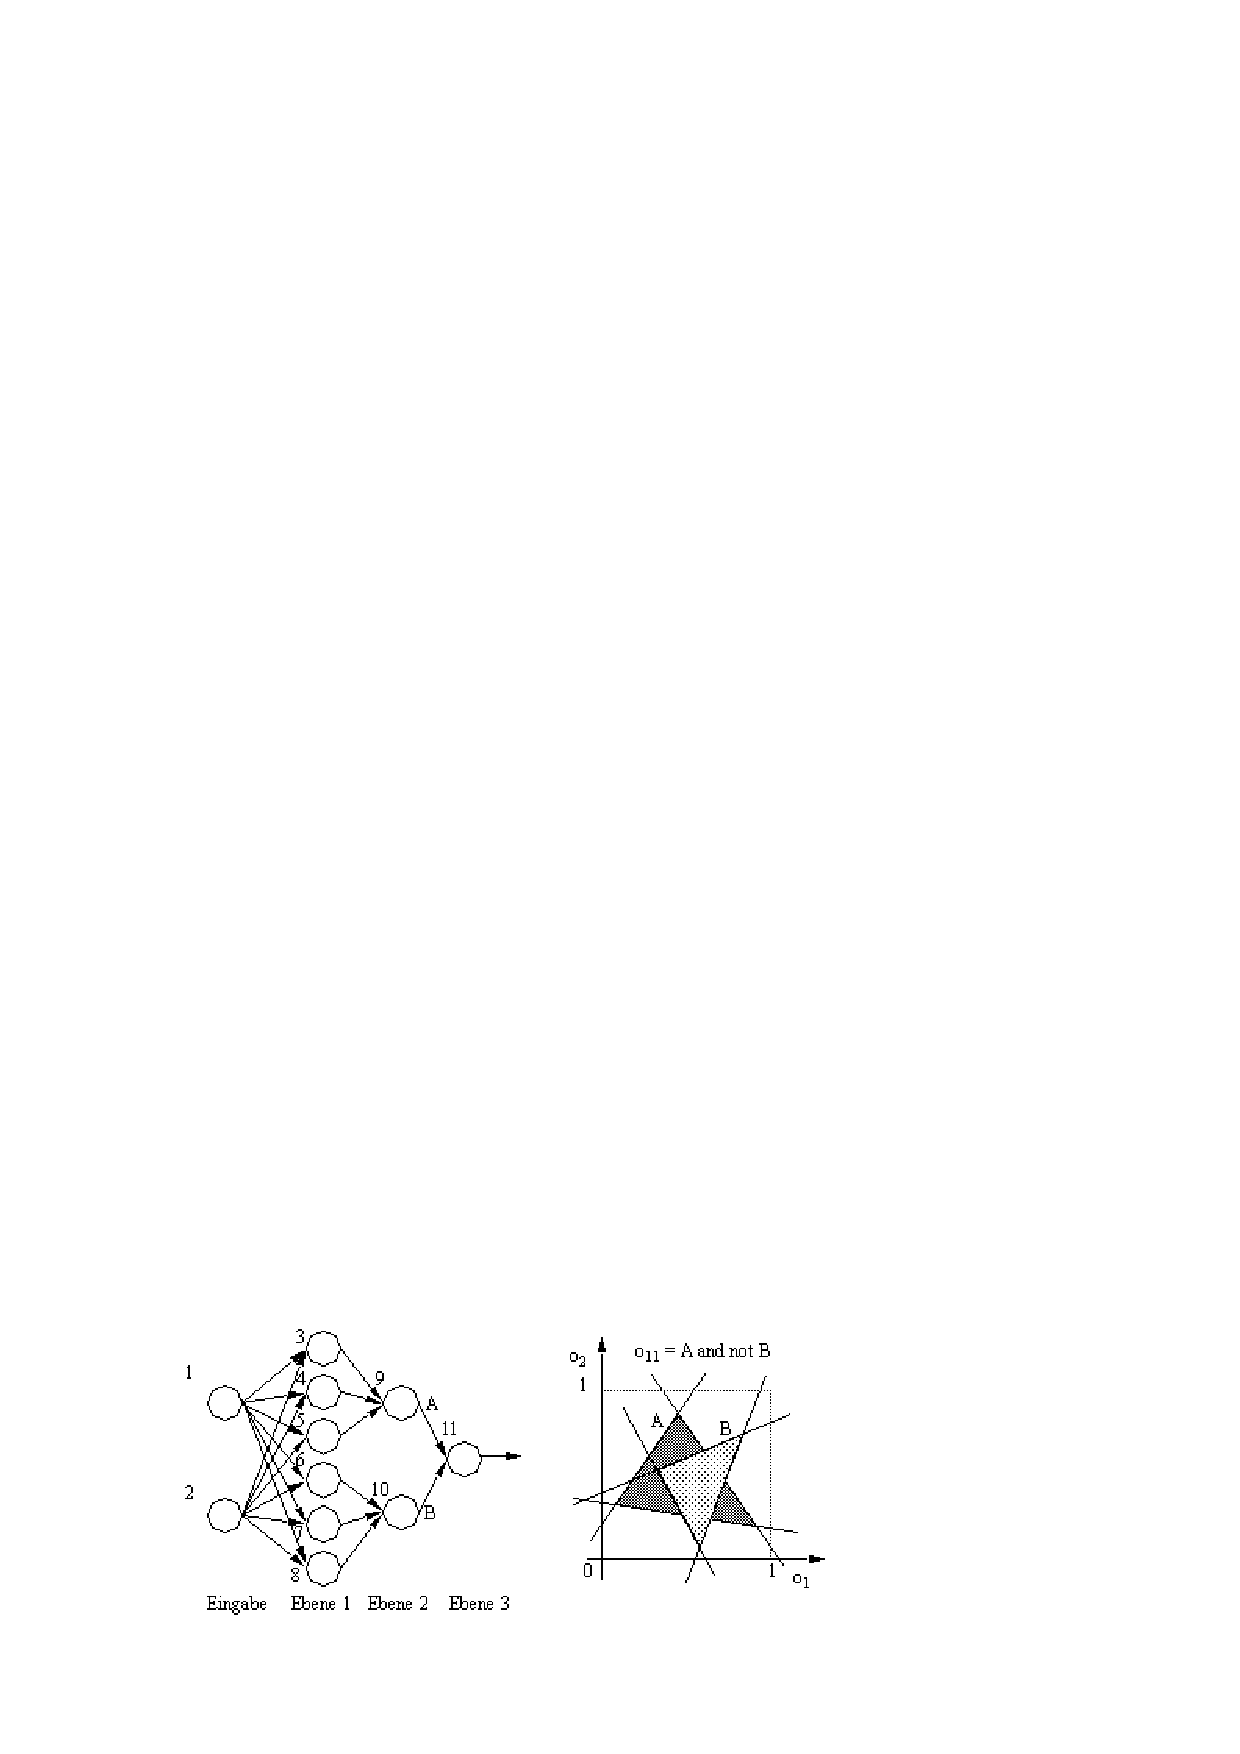
\includegraphics[width=\linewidth]{figures/ch02_perzeptron-dreistufig.pdf}
	\caption{Dreistufiges Perzeptron und ein von ihm akzeptiertes Gebiet im Merkmalsraum.}
	\label{fig:perzeptron-dreistufig}
\end{figure}

Weitere Stufen besitzen in diesem Modell keine zusätzliche Fähigkeiten mehr.


% -----------------------------------------------------------------------
% -----------------------------------------------------------------------
\section*{Lernverfahren}
Unter einem \emph{Lernverfahren} versteht man einen Algorithmus, der dem Neuronalen Netz beibringt, für einen gegebenen Merkmalsvektor $\vec{x}$ den erwarteten Wert $t$ am Ausgang $o$ zu produzieren. Ist $o = t$, dann hat das Netz erfolgreich gelernt.

Um ein Neuronales Netz zu trainieren werden dessen Gewichte angepasst. Sie \textit{speichern} das Wissen des Netzes. Diese Gewichte werden während der Traingsphase laufend angepasst. Abbildung \ref{fig:perzeptron-learning} zeigt den schematischen Lernprozess eines Perzeptrons.

\begin{figure}[ht!] \centering 
	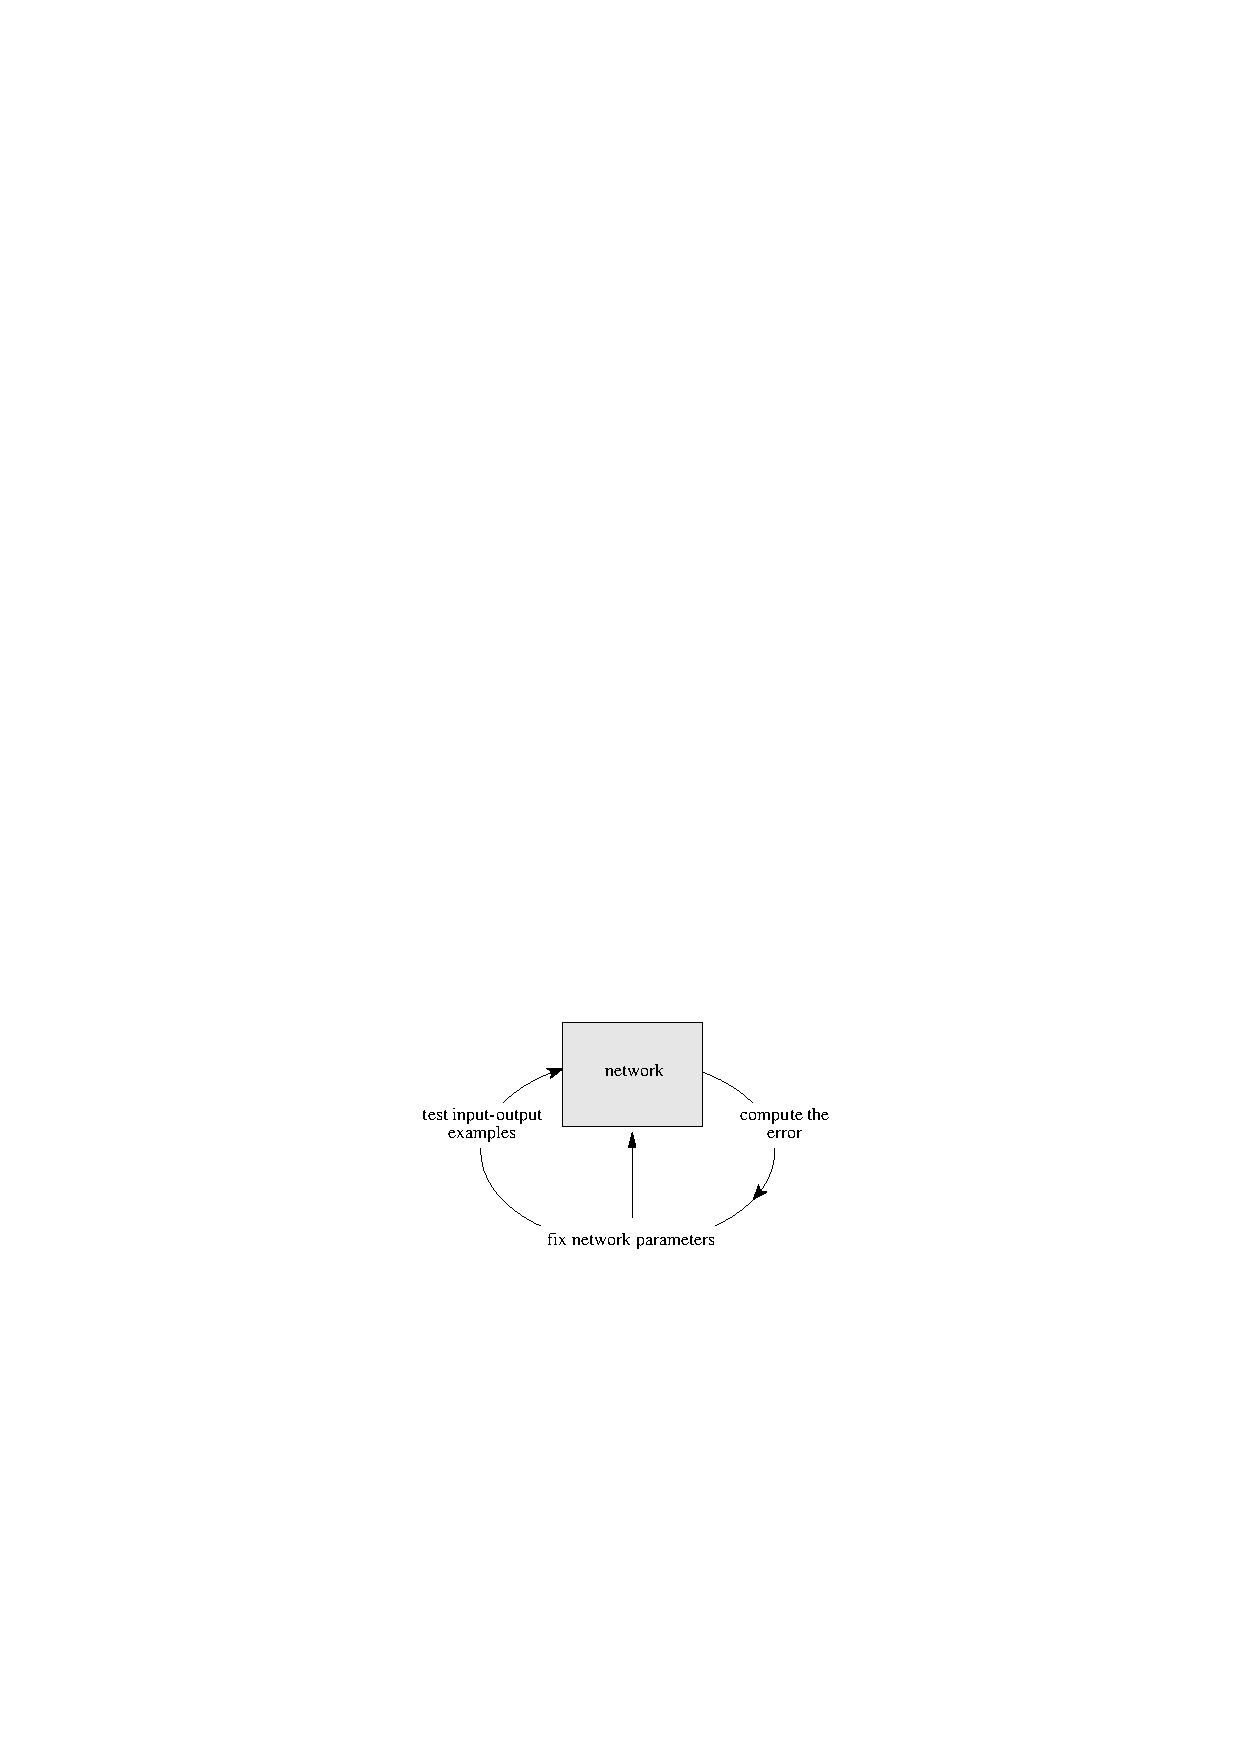
\includegraphics[width=\linewidth]{figures/ch02_perzeptron-learning.pdf}
	\caption{Schematischer Lernprozess eines Neuronalen Netzes.}
	\label{fig:perzeptron-learning}
\end{figure}

Man unterscheidet zwei Klassen von Lernalgorithmen:
\begin{itemize}
	\item \emph{überwachte Methoden} - Beim überwachten Lernen wird jedem Merkmalsvektor ein erwartetes Ergebnis zugeordnet. Lernalgorithmen beobachten die Abweichung zwischen berechnetem und erwartetem Ergebnis. Die Gewichte werden entsprechend der Größe der Abweichung angepasst. Ein solches Verfahren wird deshalb auch als \emph{Learning with a teacher} bezeichnet.
	\item \emph{unüberwachte Methoden} - Beim unüberwachten Lernen ist der genaue Ausgabewert, welcher aufgrund eines Merkmalsvektors berechnet werden soll, sowie die Anzahl und Lage der Cluster innerhalb des Merkmalsraums unbekannt. Die Trainingsmenge besteht lediglich aus Eingabemustern. Das Netzwerk muss deshalb selbst (und ohne "`teacher"') in der Lage sein, eine Klassifikation vorzunehmen. \\
	Z.B.: \emph{Self organizing maps} (SOMs)
\end{itemize}

Das \emph{überwachte} Lernen wird weiter in zwei Kategorien unterteilt:
\begin{itemize}
	\item \emph{reinforcement learning} - Hier ist nach jeder Berechnung der Ausgabe nur bekannt, ob das Netz das korrekte Ergebnis liefert oder nicht. Aufgrund dieser Informationen werden die Gewichte angepasst. Hier kann \emph{nur der Merkmalsvektor} für die Gewichtsanpassung verwendet werden.
	\item \emph{error correction} - Beim Lernen mit error correction ist die Gewichtsänderung vom Merkmalsvektor \emph{und} der Stärke der Abweichung zum gewünschten Ausgabwert abhängig.
\end{itemize}

\subsection*{Hebbsche Lernregel}
Die \emph{Hebbsche Lernregel} ist die älteste und einfachste Lernregel für Neuronale Netze. Sie besagt, dass das Gewicht zwischen zwei Einheiten dann verändert wird, wenn beide gleichzeitig aktiv sind:
\[
	\Delta w_{ij} = \eta \cdot a_i \cdot o_j
\]
Dabei ist $\Delta w_{ij}$ die Gewichtsänderung von Neuron $i$ zu Neuron $j$, $\eta$ die Lernrate, welche den Grad der Änderung bestimmt, $a_i$ die Aktivierung von Neuron $i$ und $o_j$ die Ausgabe von Neuron $j$, welches mit Neuron $i$ verbunden ist.

\subsection*{Perzeptron Lernalgorithmus}
Der Perzeptron Lernalgorithmus basiert auf der Hebbschen Regel. Gegeben ist eine Menge markierter Daten:
\[
	(x,t) \in X \times \{0,1\}
\]
Gesucht werden jene Gewichte $\hat{w}$, für die das Perzeptron alle Daten korrekt zuordnet.

Der Algorithmus berechnet für jeden Merkmalsvektor $x$ der Datenmenge $X$ die Ausgabe $o_x$ des Perzeptrons als gewichtete Summe der einzelnen Merkmale $x_j$:
\[
	o_x = \varphi(w \cdot x) = \varphi( \sum_{j=0}^{m} w_j x_j)
\]
Dabei ist $\varphi$ die Aktivierungsfunktion des Perzeptrons und $m$ die Dimension des Merkmalsraumes\footnote{Mit Bias-Trick ist $m = \text{Dimension Merkmalsraum} + 1$.}

Für das Anpassen der Gewichte gilt dann:
\begin{align*}
	&w_{t+1} =
	\begin{cases}
		w_{t} &\text{wenn } o_x = t_x \\
		w_{t} - x &\text{wenn } o_x = 1 \text{ und } t_x = 0\\
		w_{t} + x &\text{wenn } o_x = 0 \text{ und } t_x = 1
	\end{cases} \\
	&\text{alternativ auch geschrieben als:} \\
	&w_{t+1} = w_{t} + (t_x - o_x) x
\end{align*}
Wobei $w_{t}$ das aktuelle und $w_{t+1}$ das neue Gewicht ist. Entspricht die Ausgabe $o_x$ dem erwarteten Wert $t_x$, bleibt das Gewicht unverändert. Ist $o_x = 1$, sollte aber $0$ sein, wird der Merkmalsvektor abgezogen (Gewicht wird vermindert). Ist $o_x = 0$, sollte jedoch $1$ sein, wird er hinzuaddiert (Gewicht wird erhöht).
Dieser Trainingsvorgang wird so lange wiederholt, bis das Perzeptron alle Daten korrekt klassifiziert hat und damit $\hat{w}$ gefunden wurde.

Der Perzeptron Lernalgorithmus konvergiert in endlicher Zeit, wenn die Trainingsdaten linear separierbar sind (\emph{Perzeptron-Konvergenz-Theorem}). Damit kann das Perzeptron in endlicher Zeit all das lernen, was es repräsentieren kann.

Es handelt sich dabei um einen Lernalgorithmus des \emph{überwachten Lernens} mit Verstärkung (\emph{reinforcement learning}).

\subsubsection*{Pocket Perceptron Algorithm}
Ist ein Problem nicht linear separierbar, terminiert der Perzeptron Algorithmus nicht. In vielen Fällen ist es jedoch ausreichend, bei nicht pefekt linear separierbaren Problemen davon auszugehen, dass diese linear separierbar sind, weil die meisten Punkte im Merkmalsraum trotzdem richtig klassifiziert werden.
Hierfür gibt es eine Variante des Perzeptron Algorithmus: Den \emph{Pocket Perceptron Algorithm}. Dieser geht prinzipiell genau so vor wie der normale Perzeptron Algorithmus. Er merkt sich jedoch den bisher besten Gewichtsvektor.\footnote{Der beste Gewichtsvektor wird in die "`Tasche"' gesteckt. Daher der Name des Algorithmus.} Am Ende bleibt so jener Gewichtsvektor übrig, welcher am wenigsten Beispiele falsch klassifiziert.

\subsection*{Delta-Regel}
Die Delta-Regel (auch \emph{Widrow-Hoff-Regel} genannt) beruht auf dem Vergleich zwischen der gewünschten Ausgabe $t_{\Omega}$ und der tatsächlich beobachteten Ausgabe $o_{\Omega}$ eines Ausgabeneurons bzw. der tatsächlich beobachteten Aktivierung $a_{\Omega}$\footnote{Abhängig davon, ob im Teaching Input $t_{\Omega}$ die gewünschte \emph{Aktivierung} oder die gewünschte \emph{Ausgabe} hinterlegt ist.}:
\begin{align*}
	&\delta = t_{\Omega} - o_{\Omega} \\
	&\delta = t_{\Omega} - a_{\Omega}
\end{align*}
Wie auch bei der Hebbschen Lernregel gibt es drei Fälle zu unterscheiden (die beobachtete Aktivität ist zu hoch oder zu niedrig, oder entspricht dem gewünschten Ergebnis). Deshalb lautet die Formel der Delta-Regel wie folgt:
\[
	\Delta w = \eta \delta o_{\Omega}
\]
Bei der Delta-Regel ist die Gewichtsänderung aller Gewichte zu einem Ausgabeneuron $\Omega$ proportional zur Differenz der aktuellen Aktivierung $a_{\Omega}$ bzw. Ausgabe $o_{\Omega}$ und dem dazugehörigen Teaching Input $t_{\Omega}$.  

Die Delta-Regel gilt damit nur für SLPs, da sich die Formel immer auf den Teaching Input $t_{\Omega}$ bezieht und für innere Verarbeitungsschichten von Neuronen kein Teaching Input existiert. Sie wird deshalb mit dem Backpropagation-Algorithmus verallgemeinert.


\subsection*{Online- und Offline-Learning}
Der Lernvorgang kann \emph{online} und \emph{offline} erfolgen:
\begin{itemize}
	\item \emph{Online Learning} - Beim Online Learning werden die Gewichte nach jedem Beispiel aus den Trainingsdaten angepasst. Dieses Vorgehen zeichnet sich durch \emph{Schnelligkeit} aus.
	\item \emph{Offline Learning} - Beim Offline Learning hingegen werden die Gewichte nach eine Menge von Trainingsbeispielen verändert. Weshalb dieses Verfahren auch \emph{Batch-Trainingsverfahren} genannt wird, da ein Stapel Ergebnisse auf einmal korrigiert wird. Ein solcher Trainingsabschnitt wird als \emph{Epoche} bezeichnet. Dieses Vorgehen zeichnet sich durch \emph{Stabilität} aus.
\end{itemize}

\subsection*{Wichtige Fragen zum Lernen}
Fragen, über die man sich beim Lernen Gedanken machen sollte, sind im Folgenden aufgeführt.
\begin{itemize}
	\item Woher kommt die Lerneingabe und in welcher Form liegt sie vor?
	\item Wie werden die Gewichte modifiziert, um möglichst schnell und sicher zu lernen?
	\item Wie kann der Erfolg eines Lernprozesses objektiv gemessen werden?
	\item Kann ermittelt werden, welches das beste Lernverfahren ist?
	\item Kann vorhergesagt werden, ob ein Lernverfahren in endlicher Zeit terminiert?
	\item Wie wird das Gelernte im Netz gespeichert?
	\item Kann verhindert werden, dass neu gelernte Muster alte erlernte Assoziationen wieder zerstören? (\emph{Stabilitäts-Plastizitäts-Dilemma})
\end{itemize}
Diese Fragen können nicht allgemein beantwortet werden, sondern müssen für jedes Lernverfahren und jede Topologie von Netzwerk neu diskutiert werden.



% -----------------------------------------------------------------------
% -----------------------------------------------------------------------
\section*{Fehlerfunktionen}
Ein Neuronales Netz zu \emph{trainieren} heißt die Kostenfunktion (engl. cost function), also die Fehler des Netzes zu \emph{minimieren}.
Der zeitliche Verlauf des Fehlers wird als sogenannte \emph{Lernkurve} aufgetragen. Die Motivation für die Erschaffung dieser Lernkurve liegt darin, dass man mit ihr darstellen kann, ob das Netz Fortschritte macht oder nicht. Dabei sollte der Fehler normiert sein, also ein Abstandsmaß zwischen richtiger und aktueller Ausgabe des Netzes darstellen.

Man unterscheidet zwei Arten von Fehlern:
\begin{itemize}
	\item \emph{Spezifischer Fehler} $Err_p$ - Er wird über ein einziges Trainingsbeispiel, also \emph{online}, gebildet.
	\item \emph{Gesamtfehler} $Err$ - Er wird über alle Trainingsbeispiele einer Epoche, also \emph{offline}, gebildet.
\end{itemize}
Daher gilt bei $P$ Trainingsbeispielen in einer Epoche folgender Zusammenhang:
\[
	Err = \sum_{p \in P} Err_p
\]

\subsection*{Mean Squared Error (MSE)}
Der Mean-Squared-Error berechnet den spezifischen Fehler $Err_p$ anhand der quadrierten Differenz zwischen erwarteter und tatsächlicher Ausgabe.
\[
	Err_p = \frac{1}{2} \sum_{\Omega \in O} ( t_{\Omega} - o_{\Omega})^2
\]
Dabei ist $\Omega$ eines von $O$ Ausgabeneuronen. Der Vorfaktor von $\frac{1}{2}$ dient der vereinfachten Ableitung der Gleichung.

\subsection*{Euklidischer Abstand}
Der spezifische Fehler basierend auf dem euklidischen Abstand berechnet sich wie folgt.
\[
	Err_p = \sqrt{ \sum_{\Omega \in O} ( t_{\Omega} - o_{\Omega})^2 }
\]

\subsection*{Root-Mean-Square (RMS)}
Der Root-Mean-Square wird allgemein häufig verwendet, weil er auf grobe Ausreißer mehr Rücksicht nimmt.
\[
	Err_p = \sqrt{ \frac{
		\sum_{\Omega \in O} ( t_{\Omega} - o_{\Omega})^2 }
		{|O|}
		}
\]

\subsection*{Gewichtsänderung}
Die Gewichtsänderung $\Delta w$ ist proportional zur Ableitung des Fehlers nach den Gewichten. Es gilt:
\[
	\Delta w \sim - \nabla Err(w)
\]
Mit $\eta$ als Proportionalitätskonstante wir daraus:
\[
	\Delta w = - \eta \nabla Err(w)
\]
Die Ableitung der Fehlerfunktion nach den Gewichten wird im Folgenden als partielle Ableitung nach einem Gewicht $w_{i,\Omega}$ geschrieben. Umgangssprachlich formuliert wird damit an jedem Gewicht gedreht und die Änderung (Ableitung) der Fehlerfunktion betrachtet. Damit erhält man die Information $\Delta w_{i,\Omega}$, welche sagt wie das Gewicht verändert werden soll.
\[
	\Delta w_{i,\Omega} = - \eta \frac{\partial Err(w)}{\partial w_{i,\Omega}}
\]

%\section*{Aktivierungsfunktionen}
% ToDo (Hier oder in Kapitel 1.)
%\subsection*{Softmax Group Activation Function}


% ----------------------------------------------------------------------
% Themen aus Foliensatz, die in anderen Kapiteln der Zusammenfassung erläutert werden:
% ----------------------------------------------------------------------
%\subsection*{McCulloch-Pitts Neuron}
% -> Wird in Kapitel 1 der Zusammenfassung erklärt.

\section{Backpropagation}
%Kap. 8 und 9 bei Zell
% ----------------------------------------------------------------------
% ----------------------------------------------------------------------
\section*{Gradientenverfahren}
\subsection*{Gradient}
Der \emph{Gradient} ist ein Vektor $g$, der für jeden differenzierbaren Punkt einer Funktion $f$ definiert ist. Er deutet von diesem Punkt aus in die Richtung des \emph{steilsten Anstiegs} und gibt durch seinen Betrag $|g|$ den Steigungsgrad in diese Richtung an.

Der Gradient ist also die \emph{Verallgemeinerung der Ableitung für mehrdimensionale Funktionen}. Folglich deutet der negative Gradient $-g$ genau in die Richtung des steilsten Abstiegs.

Der Operator für einen Gradienten $\nabla$ wird als \emph{Nabla-Operator} bezeichnet. Die Schreibweise für einen Gradienten $g$ des Punktes $(x,y)$ einer zweidimensionalen Funktion $f$ lautet:
\[
	g(x,y) = \nabla f(x,y)
\]

\subsection*{Gradientenabstieg}
Alle Gradientenverfahren (engl. gradient descent) berechnen den Gradienten einer Zielfunktion, hier der Fehlerfunktion, und steigen entweder orthogonal zum Gradienten nach oben, bis ein Maximum erreicht ist oder nach unten, bis ein Minimum erreicht ist.
Hier wird versucht, durch Änderung der Gewichte den Fehler zu minimieren, indem eine Änderung aller Gewichte um einen Bruchteil des negativen Gradienten der Fehlerfunktion vorgenommen wird.
Es gilt der Zusammenhang, welcher schon im vorherigen Abschnitt bei den Fehlerfunktionen behandelt wurde:
\begin{align*}
	\Delta w &= - \eta \nabla Err(w) \\
	\Delta w_{i,\Omega} &= - \eta \frac{\partial Err(w)}{\partial w_{i,\Omega}}
\end{align*}

\begin{figure}[ht!] \centering 
	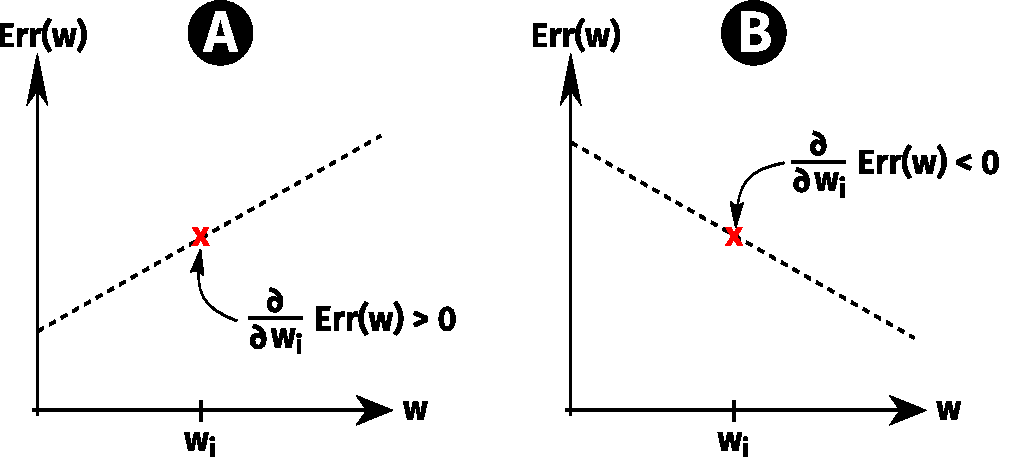
\includegraphics[width=\linewidth]{figures/ch03_gradient-decent.pdf}
	\caption{Gradientenabstieg grafisch dargestellt. Im Fall \emph{A} ist die Steigung der Fehlerfunktion beim Gewicht $w_i$ positiv, das Gewicht muss demnach verkleinert werden, damit der Fehler kleiner wird. Im Fall \emph{B} hingegen ist die Steigung bei $w_i$ negativ, das Gewicht muss dementsprechend erhöht werden, um die Kosten zu reduzieren. Dies ist der Grund für das Minuszeichen in der Gleichung.}
	\label{fig:ch03_fehlerflaeche}
\end{figure}

Auch beim Gradientenabstiegsverfahren unterscheidet man zwischen online und offline Verfahren: 
\begin{itemize}
	\item \emph{Stochastic Gradient Descent} - Die Anpassung der Gewichte findet nach jedem Trainingsbeispiel statt. Daher ist dieses Verfahren robuster gegen nicht-konvexe Fehlerfunktionen. 
	\item \emph{Batch Gradient Descent} - Hier werden die Änderungen der Gewichte über eine Epoche hinweg aufaddiert und erst anschließend auf die Gewichte angewandt.
\end{itemize}



% ----------------------------------------------------------------------
% ----------------------------------------------------------------------
\section*{Prinzip von Backpropagation}
Backpropagation ist ein \emph{Gradientenabstiegsverfahren} und die Erweiterung der Delta-Regel auf mehrere trainierbare Gewichtsschichten, weil bei mehrstufigen Netzen keine erwünschte Ausgabe als Lerneingabe (teaching input) für die Zellen \emph{innerer Ebenen} vorhanden ist.

Wenn man den Fehler eines neuronalen Netzes als Funktion der Gewichte des Netzwerks graphisch aufträgt, erhält man eine Fehlerfläche, welche sich im zweidimensionalen Fall anschaulich graphisch darstellen lässt.

\begin{figure}[ht!] \centering 
	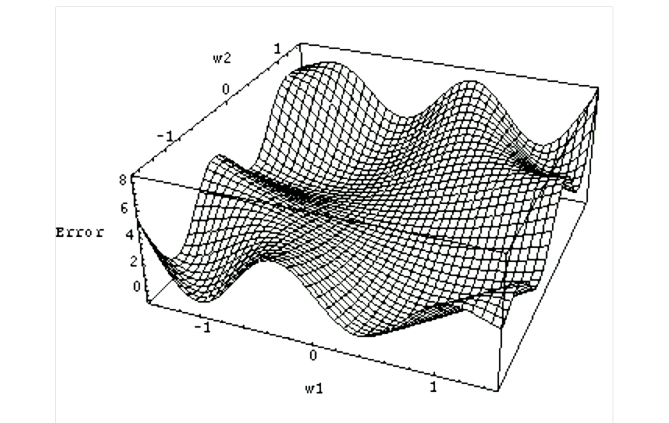
\includegraphics[width=\linewidth]{figures/ch03_fehlerflaeche.pdf}
	\caption{Fehlerfunktion $Err(w_1, w_2)$ grafisch aufgetragen.}
	\label{fig:ch03_fehlerflaeche}
\end{figure}

Abbildung \ref{fig:ch03_fehlerflaeche} zeigt die Fehlerfunktion $Err(w_1, w_2)$. Bei $n$ Gewichten gilt allgemein:
\[
	Err(\vec{w}) = Err(w_1, \ldots, w_n)
\]
Diese Fehlerfunktion gibt den Fehler an, den das Netz bei gegebenen Gewichten $w_1, \ldots, w_n$ über alle Trainingsmuster aufsummiert besitzt.

Mit einem Gradientenverfahren, d.h. der Methode des steilsten Abstiegs, wird nun versucht, möglichst schnell ein globales Minimum der Fehlerfunktion zu finden, d.h. eine Konfiguration der Gewichte, bei der die Fehlersumme über alle Trainingsmuster minimal ist.



% ----------------------------------------------------------------------
% ----------------------------------------------------------------------
\section*{Verallgemeinerung der Delta-Regel}
Zur Veranschaulichung der verallgemeinerten Delta-Regel, genannt \emph{Backpropagation of Error} oder kurz \emph{Backpropagation} dient das in Abbildung \ref{fig:ch03_fehlerflaeche} dargestellte Multi-Layer-Perzeptron (MLP).
Formal ergibt sich daraus folgender Zusammenhang:
\begin{align*}
	\Delta w_{k,h} &= \eta \cdot o_k \cdot \delta_h \\
	&\text{mit} \\
	\delta_h &=
	\begin{cases}
		f'_{act}(net_h) \cdot (t_h - y_h) 
		\quad &\text{wenn h außen} \\
		f'_{act}(net_h) \cdot \sum_{l \in L} (\delta_l \cdot w_{h,l})
		\quad &\text{wenn h innen}
	\end{cases}
\end{align*}

\begin{figure}[ht!] \centering 
	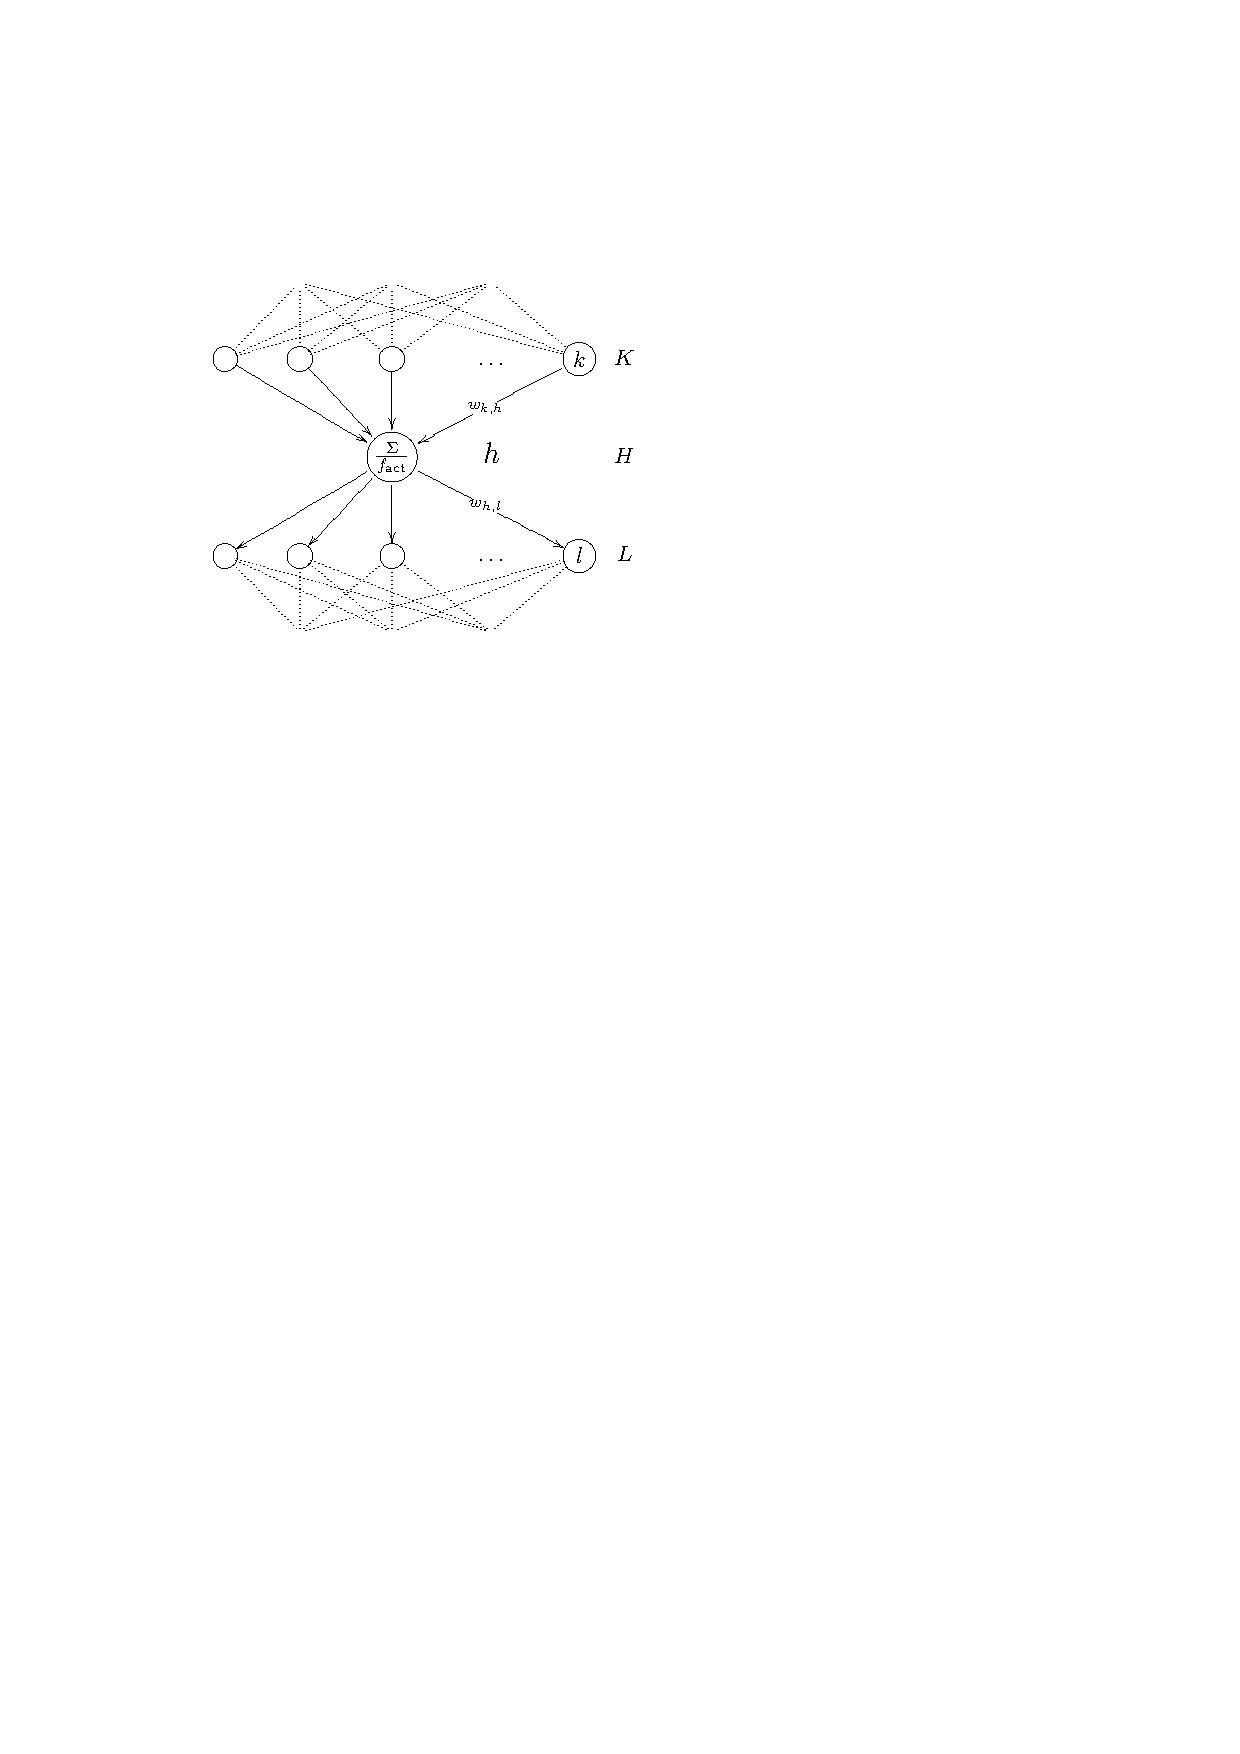
\includegraphics[width=\linewidth]{figures/ch03_mlp-backpropagation.pdf}
	\caption{Diese Abbildung zeigt die Lage des in der Formel für Backpropagation betrachteten Neurons $h$ in einer Hiddenschicht $H$. Die Vorgängerschicht ist $K$, die nachfolgende Schicht $L$. Wichtig hierbei: $L$ ist \emph{nicht} die Ausgabeschicht, sonst würde für $h$ die einfache Delta-Regel gelten.}
	\label{fig:ch03_fehlerflaeche}
\end{figure}



% ----------------------------------------------------------------------
% ----------------------------------------------------------------------
\section*{Aktivierungsfunktionen für Backpropagation}
Aus der Formel für Backpropagation geht hervor, dass die Aktivierungsfunktion semilinear, d.h. monoton und differenzierbar, sein muss. Darüber hinaus muss gelten:
\[
	f'_{act} \ne 0
\]
Werden diese Eigenschaften nicht erfüllt, so ist das Produkt für $\delta_h$ stets $0$. Eine Gewichtsänderung kann dann nicht statt finden. Deshalb eignet sich die Schrittfunktion nicht als Aktivierungsfunktion für Backpropagation.

\subsection*{Sigmoid-Aktivierungsfunktion}
Häufig wird stattdessen die Sigmoid-Aktivierungsfunktion verwendet, wie sie in Abbildung \ref{fig:ch03_sigmoid} dargestellt ist. Sie ist definiert durch:
\[
	s(x) = \frac{1}{1 + e^{-cx}} \\
\]
Für die Ableitung gilt:
\[
	\frac{d}{dx} s(x) = \frac{e^{-x}}{(1 + e^{-x})^2} = s(x)(1-s(x))
\]

\begin{figure}[ht!] \centering 
	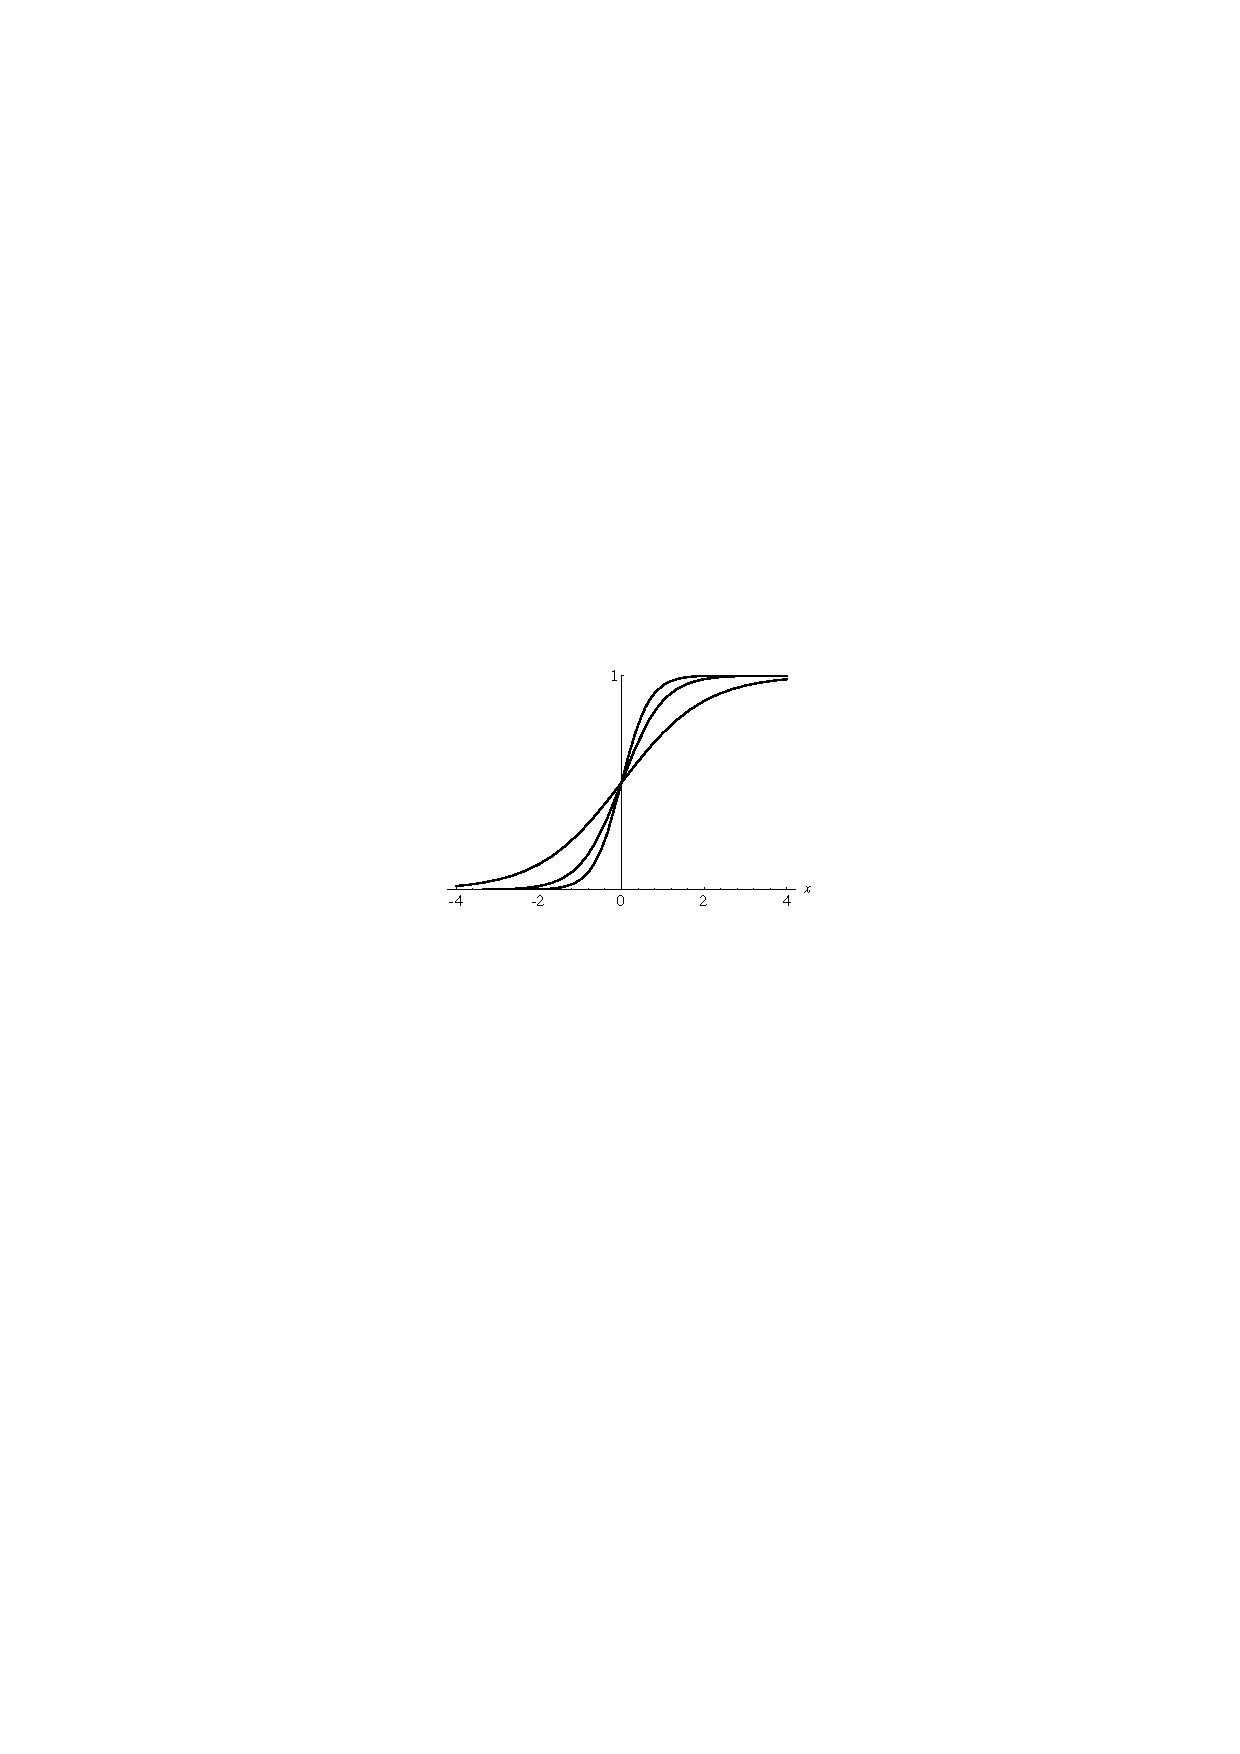
\includegraphics[width=0.7\linewidth]{figures/ch03_sigmoid.pdf}
	\caption{Verlauf der Sigmoid-Aktivierungsfunktion für $c=1$, $c=2$ und $c=3$. Je größer $c$ gewählt wird, desto steiler ist der Anstieg von $0$ auf $1$.}
	\label{fig:ch03_sigmoid}
\end{figure}



% ----------------------------------------------------------------------
% ----------------------------------------------------------------------
\section*{Algorithmus}
Im Folgenden ist der Ablauf des Backpropagation-Algorithmus aufgeführt.

\begin{itemize}
	\item zufällige Initialisierung der Gewichte
	\item Wahl eines Eingabemusters $x \in X$

	\begin{itemize}
		\item \emph{Forward propagation}: \\
			Berechnung der Netzausgabe $o_x$
		\item \emph{Backward propagation}: \\
			Fehlerrückführung durch das Netz und Berechnung des Fehleranteils je Gewicht: \\
			$\quad \frac{\partial Err(W)}{\partial w_{k,h}}
				(= - \delta_h \cdot o_k) $

		\begin{itemize}
			\item Für Ausgabeneuronen: \\
				$\delta_h = 
				\underbrace{(o_{x,h}(1-o_{x,h})}_{f'_{act}(net_{x,h})} 
				\cdot (t_{x,h}-y_{x,h})$ 
			\item Für versteckte Neuronen: \\
				$\delta_h = 
				\underbrace{(o_{x,h}(1-o_{x,h})}_{f'_{act}(net_{x,h})} 
				\sum_{l \in L} \delta_l \cdot w_{h,l}$ 
		\end{itemize}

		\item Anpassen der Gewichte: $w_{k,h} \leftarrow w_{k,h} + \eta o_k \delta_h$ 
		\item Solange wiederholen, bis Ergebnis (zu einem lokalen Minimum) konvergiert.
	\end{itemize}

\end{itemize}


% ----------------------------------------------------------------------
% ----------------------------------------------------------------------
\section*{Probleme}
Wie jedes Gradientenverfahren besitzt auch Backpropagation eine Reihe von Problemen, die dadurch entstehen, dass es ein lokales Verfahren ist, welches keine Information über die Fehlerfläche insgesamt hat, sondern nur aus der Kenntnis der lokalen Umgebung (des Gradienten bzw. bei Erweiterungen des Verfahrens zusätzlich einiger vorher besuchter Stellen der Fehlerfläche) ein Minimum suchen muss.

\begin{figure}[ht!] \centering 
	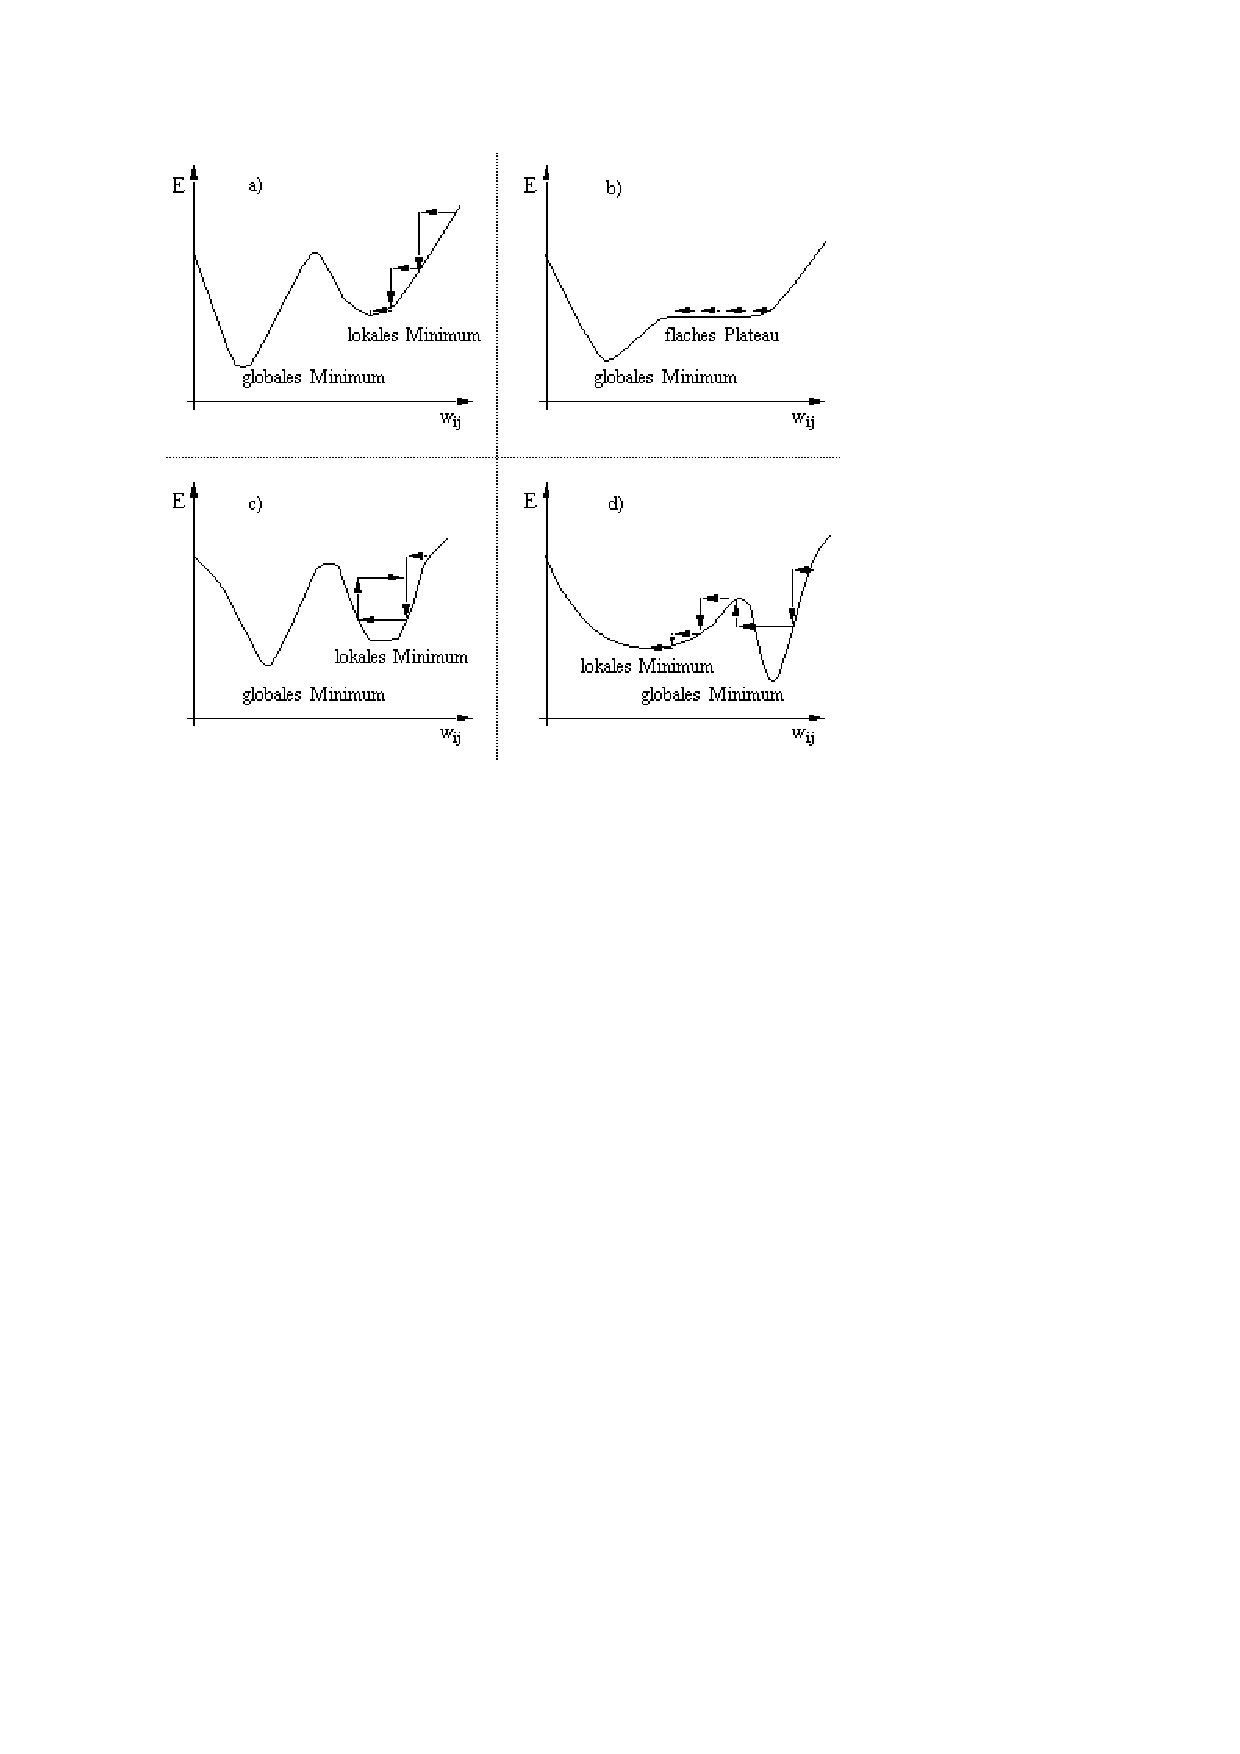
\includegraphics[width=\linewidth]{figures/ch03_fehler-gradientenverfahren.pdf}
	\caption{Problemfälle von Gradientenverfahren: a) lokales Minimum einer Fehlerfläche, b) Fehlerfläche mit Plateau, c) Oszillationen in steilen Schluchten der Fehlerfläche, d) Verlassen guter Minima}
	\label{fig:ch03_sigmoid}
\end{figure}

\subsection*{Lokale Minima der Fehlerfläche}
Gradientenverfahren haben alle das Problem, dass sie in einem lokalen Minimum der Fehlerfläche hängenbleiben können.
Das Problem neuronaler Netze ist, dass die Fehlerfläche mit wachsender Dimension des Netzes (mit wachsender Zahl von Verbindungen) immer stärker zerklüftet wird und daher die Wahrscheinlichkeit, in einem lokalen statt dem globalen Minimum zu landen, immer größer wird.

Zur Lösung solcher Probleme gibt es wenig allgemeingültigen Verfahren, weil sie stark von der Anwendung abhängen.
Die Erfahrung in der Praxis hat jedoch gezeigt, dass Backpropagation bei genügend kleiner Lernrate $\eta$ in sehr vielen Anwendungen ein Minimum findet, das gut genug am globalen Minimum liegt.

\subsection*{Flache Plateaus}
Flache Plateaus der Fehlerfläche sind ein weiteres Problem von Gradientenverfahren. Da die Größe der Gewichtsänderung von dem Betrag des Gradienten abhängig ist, stagniert Backpropagation auf flachen Plateaus, d.h. das Lernverfahren braucht extrem viele Iterationsschritte. 
Handelt es sich um ein vollständig flaches Plateau, ist der Gradient gleich dem Nullvektor und eine Gewichtsänderung findet gar nicht mehr statt.
Einen solchen Stillstand kann man dann nur schwer von dem in einem lokalen oder globalen Minimum unterscheiden, weil auch dort der Gradient ebenfalls der Nullvektor ist.

Für dieses Problem gibt es mit dem \emph{Momentum-Term}, einer Variante von Backpropagation, ein einfaches Verfahren, welches hilft diese Plateaus zu überwinden.

\subsection*{Oszillationen in steilen Schluchten}
In steilen Schluchten der Fehlerfläche kann das Lernverfahren oszillieren. Dies geschieht, wenn der Gradient am Rande einer Schlucht so groß ist, dass durch die Gewichtsänderung ein Sprung auf die gegenüberliegende Seite der Schlucht erfolgt. Ist die Schlucht dort genauso steil, bewirkt dies (da der Gradient jetzt in die andere Richtung zeigt) einen Sprung zurück auf die erste Seite.

Auch hier hilft der Momentum-Term.

\subsection*{Verlassen guter Minima}
Es ist möglich, in der Praxis aber sehr selten, dass Backpropagation aus einem guten Minimum herausspringt, weil der Betrag des Gradienten innerhalb eines sehr engen Tals der Fehlerfläche so groß ist, dass die Gewichtsänderung in ein suboptimales Minimum führt.

Gerade die Verwendung des Momentum-Terms oder die Erhöhung der Lernrate führen zu solchen Problemen.

\subsection*{Wahl der Lernrate}
Die Wahl der Lernrate $\eta$ (Schrittweite) ist entscheidend für das Verhalten des Backpropagation-Algorithmus. Zu große Werte von $\eta$ bewirken starke Sprünge auf der Fehlerfläche und bringen das Risiko mit sich, dass Backpropagation enge Täler nicht findet bzw. dass es aus ihnen wieder herausspringt oder ins Oszillieren gerät.
Zu kleine Werte von $\eta$ bringen einen großen, oft praktisch nicht akzeptierbaren Zeitaufwand für das Training mit sich.

Die Wahl von $\eta$ hängt vom Problem, den Trainingsdaten, sowie der Größe und Topologie des Netzes ab und ist nicht pauschal zu beantworten. Es gibt Verfahren zur Anpassung der Lernrate, welche in einem eigenen Abschnitt erläutert werden.



% ----------------------------------------------------------------------
% ----------------------------------------------------------------------
\section*{Modifikationen von Backpropagation}
\subsection*{Momentum-Term}
Backpropagation mit Momentum-Term (auch konjugierter Gradientenabstieg (engl. conjugate gradient descent)) wurde von Rumelhart, Hinton und Williams beschrieben.
Es ist eine einfache und häufig benutzte Methode zur Vermeidung der Probleme von Backpropagation auf flachen Plateaus und in steilen Schluchten der Fehlerfunktion. 

Die Idee dahinter ist das Einbeziehen der vorangegangenen Gewichtsänderung. Dies führt zu einer \emph{Beschleunigung} (Erhöhung der Gewichtsänderung $\Delta w_{i,j}$) in weiten Plateaus und zu einem \emph{Abbremsen} in stark zerklüfteten Fehlerflächen.

Für die Gewichtsänderung gilt dann:
\[
	\Delta w_{i,j} (t+1) = \eta \cdot o_i \cdot \delta_j + 
		\alpha w_{i,j}(t)
\]

\begin{figure}[ht!] \centering 
	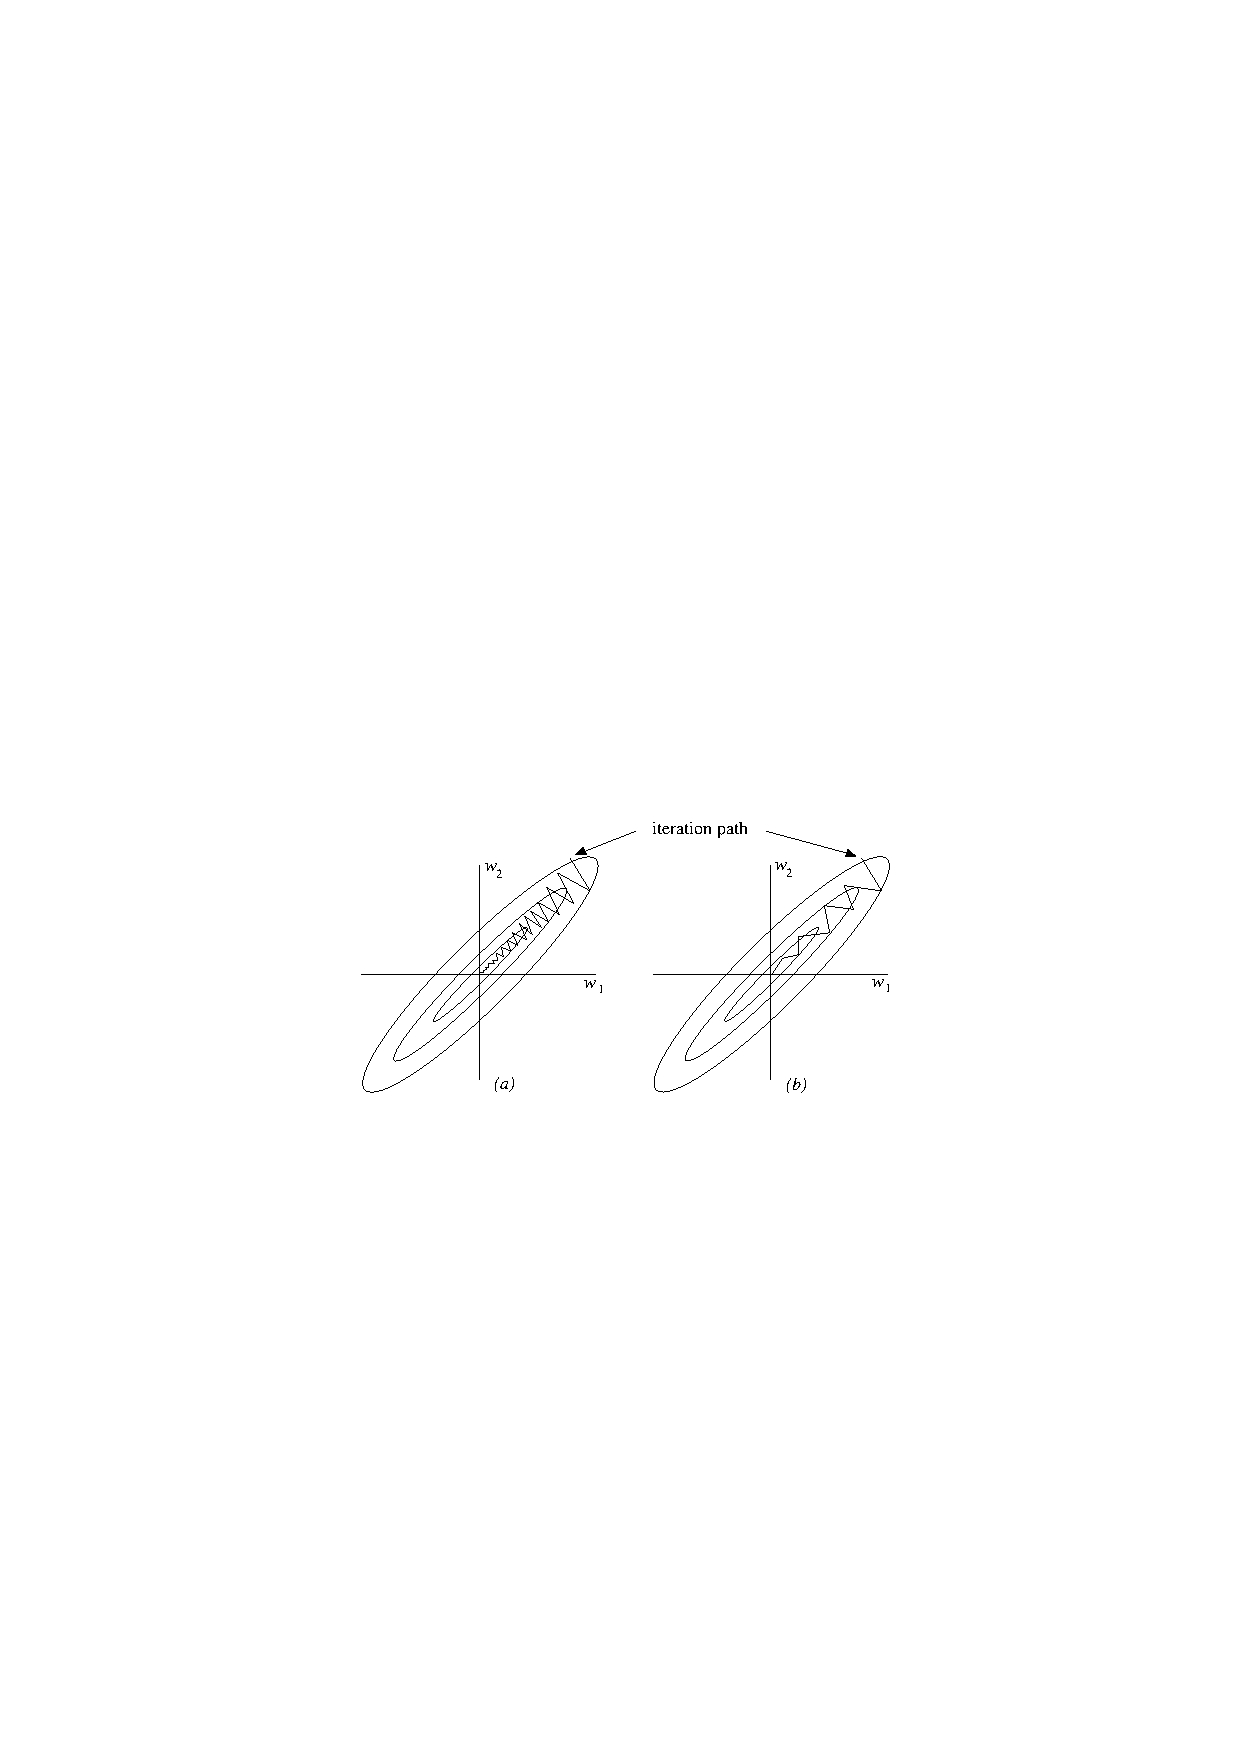
\includegraphics[width=\linewidth]{figures/ch03_momentum-term.pdf}
	\caption{Backpropagation ohne (a) und mit (b) Momentum-Term.}
	\label{fig:ch03_momentum-term}
\end{figure}

\subsection*{Flat-Spot Elimination}
Ein bekanntes Problem der Backpropagation-Formel ist die Tatsache, dass Neuronen, die im Sättigungsbereich der sigmoiden Aktivierungsfunktion operieren (0 oder 1 bei der logistischen Aktivierungsfunktion), sich nur schwer wieder daraus entfernen, weil ihre Gewichte sich nur um einen minimalen Bruchteil ändern können.

Die Ableitung der Sigmoid-Funktion ist für Neuronen, die stark "`an"' oder "`aus"' sind, d.h. Werte um 0 oder 1 annehmen, nahezu Null. Diese Bereiche, in dem die Ableitung der Aktivierungsfunktion fast Null ist, werden daher \emph{flat spots} genannt (siehe Abbildung \ref{fig:ch03_saettigung-sigmoid-ableitung}.\footnote{Selbst im besten Fall, wenn die Netzeingabe um den Schwellenwert liegt, liefert die Ableitung der Aktivierungsfunktion einen gedämpften Faktor von $0,25$.}

\begin{figure}[ht!] \centering 
	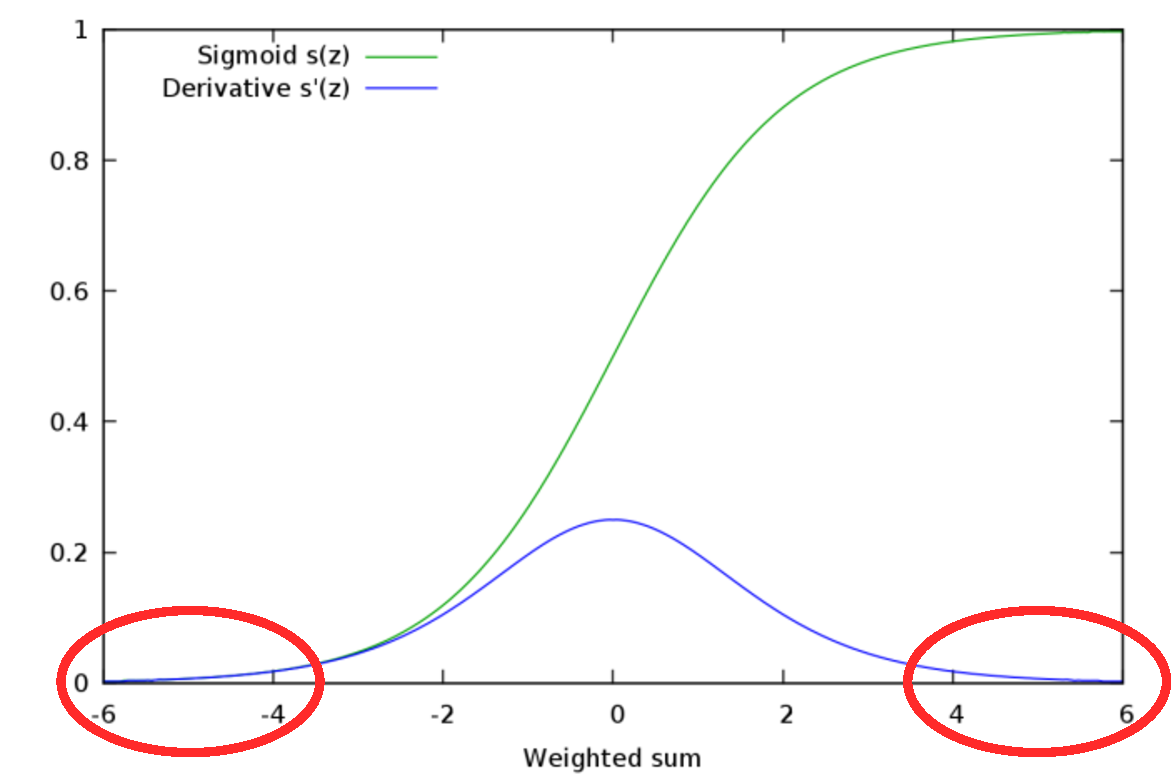
\includegraphics[width=\linewidth]{figures/ch03_saettigung-sigmoid-ableitung.pdf}
	\caption{Ableitung der Sigmoid-Funktion mit Sättigungsbereichen / \emph{flat spots} (gekennzeichnet durch Kreise).}
	\label{fig:ch03_saettigung-sigmoid-ableitung}
\end{figure}

Ein einfache Methode, dieses Problem zu beheben, ist die Anpassung der Ableitung, sodass sie nicht Null wird. Dies ist beispielsweise durch Addition einer Konstanten $0.1$ für alle Werte möglich.
Damit verläuft die Ableitung anstelle von $0$ bis $0.25$ und zurück auf $0$ jetzt von $0.1$ bis $0.35$ und zurück auf $0.1$.
In der Literatur wird diese Variante auch als \emph{modified sigmoid-prime function} bezeichnet.


\subsection*{Manhattan-Training}
Die sogenannte Manhattan-Training-Modifikation von Backpropagation geht auf Bart Sutton zurück. Dabei wird die Backpropagation-Regel durch die Regel
\[
	\Delta w_{i,j} = \eta \cdot o_i \cdot sgn( \delta_j)
\]
ersetzt, wobei die Berechnung der Fehlersignale wie bei der verallgemeinerten Delta-Regel erfolgt. Bei dieser Regel spielen nicht mehr die Beträge der Fehlersignale eine Rolle, sondern nur noch ihr \emph{Vorzeichen}. Dadurch werden die \emph{Schritte auf der Fehlerfläche quasi-normiert}, was den Problemen zu kleiner Gradienten bei flachen Plateaus und zu großer Gradienten in steilen Tälern entgegenwirkt.

Diese Quasi-Normierung ist wesentlich weniger rechenzeitaufwendig als eine richtige Normierung des Gradienten $\nabla E$ auf eine feste Länge und daher dieser meist vorzuziehen.


\subsection*{SuperSAB}
Bei SuperSAB hat jedes Gewicht eine eigene Lernrate / Schrittweite $\eta_{i,j}(t)$. Diese wird im Verlauf des Trainings kontinuierlich der Fehlerfläche angepasst. Dabei wird $\eta_{i,j}$ vergrößert, wenn die partielle Ableitung $\frac{\partial Err_p}{\partial w_{i,j}}$ für mehrere Zeitschritte das gleiche Vorzeichen hat und verkleinert, wenn sich das Vorzeichen ändert.

Für die Anpassung wird das Produkt aus der aktuellen Lernrate $\eta_{i,j}(t)$, sowie einer der Konstanten $\eta^-$ (meist $0.5$) oder $\eta^+$ (meist $1.05$) verwendet:
\begin{align*}
	\eta_{i,j}(t+1) = 
	\begin{cases}
		\eta_{i,j}(t) \cdot \eta^- &\text{falls }
			\frac{\partial E}{\partial w_{i,j}}(t) \cdot
			\frac{\partial E}{\partial w_{i,j}}(t+1) < 0 \\
		\eta_{i,j}(t) \cdot \eta^+ &\text{falls }
			\frac{\partial E}{\partial w_{i,j}}(t) \cdot
			\frac{\partial E}{\partial w_{i,j}}(t+1) > 0 \\
		\eta_{i,j}(t) &\text{sonst}
	\end{cases}
\end{align*}


\subsection*{Quickprop}
Mit dem Quickprop-Algorithmus soll eine schnelleres Training eines MLP erreicht werden. Er macht zwei "`riskante"' Annahmen:
\begin{enumerate}
	\item Die Fehlerkurve $Err(w)$ hat die Form einer Parabel
	\item Die Parabeln für jedes Gewicht $w_{h,l}$ sind unabhängig von einander.
\end{enumerate}
Diese Annahmen sind nicht richtig. Durch das iterative Einstellen der Gewichte werden die gemachten Fehler jedoch aufgehoben.

Der Algorithmus wird manchmal der Gruppe Lernverfahren zweiter Ordnung zugerechnet, da über eine \emph{quadratische} Approximation aus dem vorhergehenden Gradientenschritt $S(t-1)$ und dem aktuellen Gradienten $S(t)$ auf das Minimum der Fehlerfunktion (Scheitelpunkt der Parabel) geschlossen wird (siehe Abbildung \ref{fig:ch03_quickprop}).

Aus Abbildung \ref{fig:ch03_quickprop} geht hervor, dass die Gewichtsänderung $\Delta w_{ij}(t)$ gesucht ist, um das neue Gewicht zum Zeitpunkt $t+1$ zu bestimmen (Gewicht am Scheitelpunkt der Parabel). Aus den Ähnlichkeiten der schraffiert hervorgehobenen Dreiecke folgt dieser Zusammenhang:
\[
	\frac{\Delta w_{i,j}(t)}{\Delta w_{i,j}(t-1)} = 
		\frac{S(t)}{S(t-1) - S(t)}
\]
Daraus ergibt sich für die Gewichtsänderung $\Delta w_{i,j}(t)$ und damit für den Quickprop-Algorithmus diese Gleichung:
\[
	\Delta w_{i,j}(t) = 
		\frac{S(t)}{S(t-1) - S(t)} \cdot \Delta w_{i,j}(t-1)
\]

\begin{figure}[ht!] \centering 
	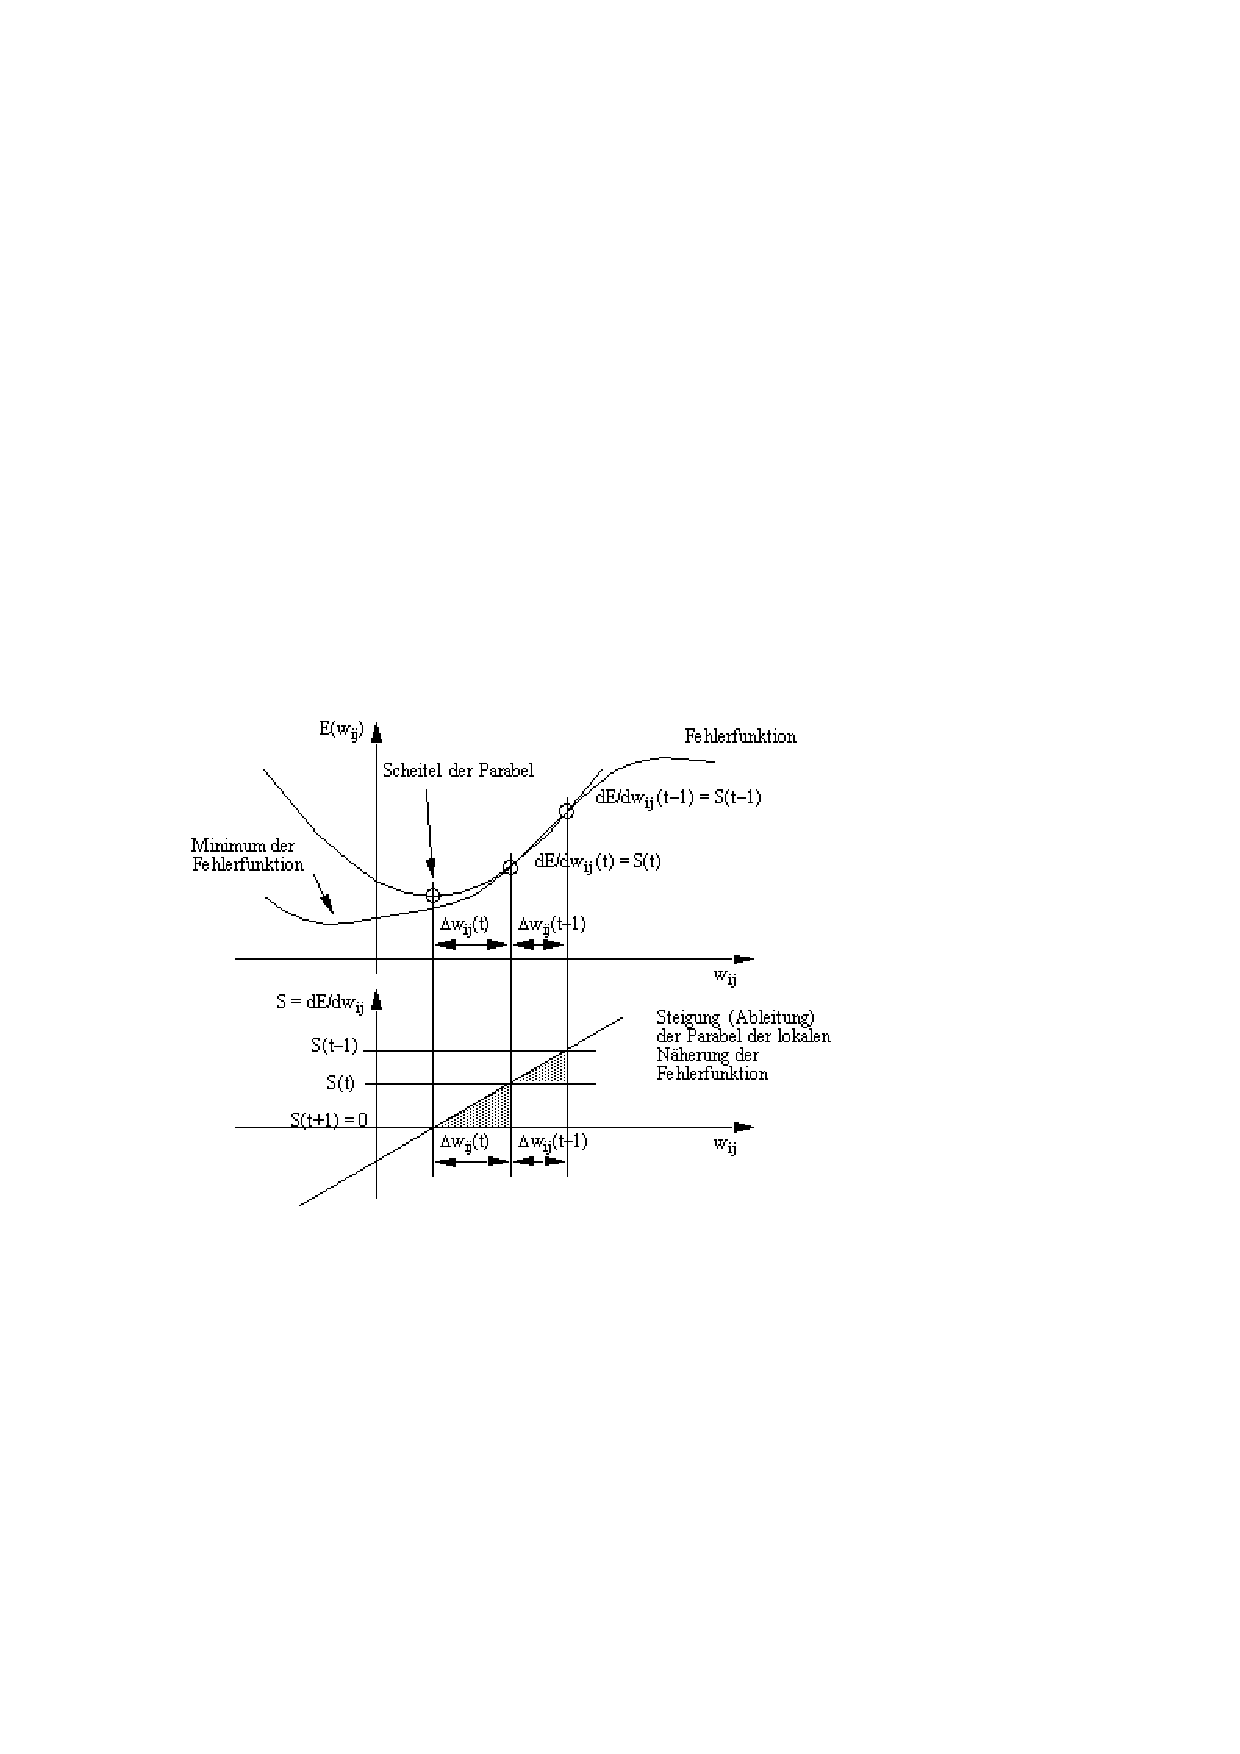
\includegraphics[width=\linewidth]{figures/ch03_quickprop.pdf}
	\caption{Idee des Quickprop-Algorithmus: Bestimmung des Scheitelpunktes der angelegten Parabel anhand der Steigung zweier verschiedener Punkte und deren Abstand. Die Abbildung zeigt oben die Fehlerkurve mit angenäherter Parabel, sowie die beiden Punkte zum Zeitpunkt $t-1$ und $t$. Unten ist die Steigung der Parabel als Gerade durch die beiden Steigungswerte $S(t-1)$ und $S(t)$ aufgetragen. Die Nullstelle gibt das Gewicht für den (angenäherten) minimalen Fehler (Scheitelpunkt der Parabel im oberen Diagramm) an.}
	\label{fig:ch03_quickprop}
\end{figure}



Der Quickprop-Algorithmus funktioniert sehr gut für hochgradig nichtlineare Probleme wie z.B. XOR. Ein beispielhaftes Trainingsverhalten ist in Abbildung \ref{fig:ch03_quickprop-training} aufgeführt.

\begin{figure}[ht!] \centering 
	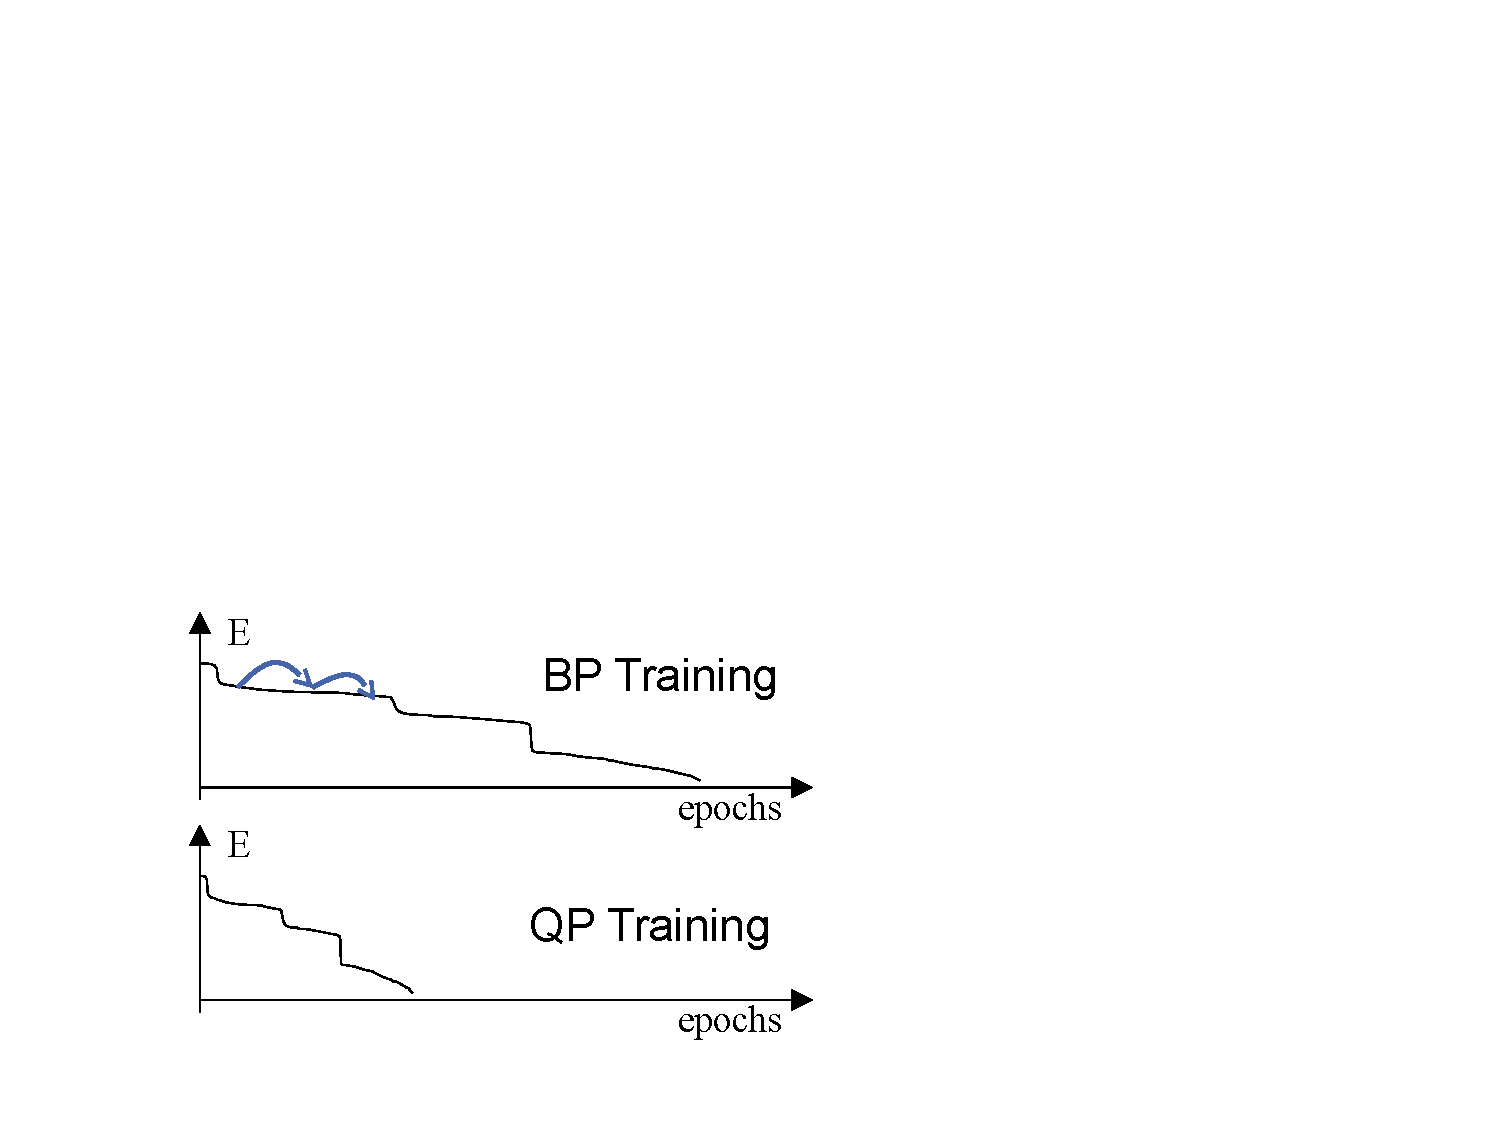
\includegraphics[width=0.7\linewidth]{figures/ch03_quickprop-training.pdf}
	\caption{Trainingsverhalten von Backpropagation (oben) und Backpropagation mit Quickprop (unten) bei hochgradig nichtlinearen Problemen.}
	\label{fig:ch03_quickprop-training}
\end{figure}

\subsection*{Rprop}
Rprop (resilient propagation) ist ein Lernverfahren, das Ideen des Manhattan-Trainings, von SuperSAB und von Quickprop kombiniert: Um die Gewichte zu aktualisieren wird nur die Lernrate $\eta$ und das Vorzeichen der partiellen Ableitung $\frac{\partial E}{\partial w_{i,j}}$ verwendet.

Dieses Vorgehen beschleunigt den Lernvorgang insbesondere in flachen Ebenen der Fehlerfunktion und nahe von lokalen Minima. Um eine zu starke Be- bzw. Entschleunigung zu verhindern existieren Minimal- und Maximalwerte ($\eta_{min}$ und $\eta_{max}$) für die Lernrate.

Wie beim Manhattan-Training werden die Gewichte nicht nach dem Gradienten der Fehlerfunktion, sondern \emph{nur nach dem Vorzeichen dieses Gradienten} geändert.
Für die Gewichts"-änderung bei Rprop gilt demnach:
\begin{align*}
	\text{es sei } g &= \frac{\partial Err(W)}{\partial w_{i,j}}\\\\
	\Delta w_{i,j} (t) &=
	\begin{cases}
		-\eta_{i,j} (t) &\text{wenn } g(t) > 0 \\
		+\eta_{i,j} (t) &\text{wenn } g(t) < 0 \\
		0 &\text{sonst} 
	\end{cases}
\end{align*}

Wie bei SuperSAB und bei Quickprop werden die Steigungen der Fehlerfunktion des aktuellen und vorherigen Zeitpunkts verwendet.
Ähnlich wie bei SuperSAB besitzt jedes Gewicht einen eigenen Parameter für die Änderung der Schrittweite.
Für die Anpassung der Lernrate $\eta_{i,j}$ wird der aktuelle Gradient $g(t)$ und der vorherige Gradient $g(t-1)$ betrachtet. Wieder ist das Vorzeichen entscheidend: Es kann über die beiden Zeitschritte gleich bleiben oder wechseln.

Wechselt das Vorzeichen von $g(t-1)$ zu $g(t)$, wurde ein lokales Minimum übersprungen, die Gewichtsänderung war zu groß.
Folglich muss die Lernrate $\eta_{i,j}(t)$ im Vergleich zu $\eta_{i,j}(t-1)$ \emph{verkleinert} werden. Dies geschieht (analog zu SuperSAB) durch Multiplikation des alten Wertes $\eta_{i,j}(t-1)$ mit der Konstanten $\eta^-$.

Bleibt das Vorzeichen jedoch gleich, kann eine (behutsame) Vergrößerung durch Multiplikation von $\eta_{i,j}(t-1)$ mit der Konstanten $\eta^+$ vorgenommen werden. Dies hilft um über flache Bereiche der Fehlerfunktion hinwegzukommen.

Für die Anpassung der Lernrate gilt bei Rprop also:
\begin{align*}
	\eta_{i,j}(t) = 
	\begin{cases}
		\eta^+ \cdot \eta_{i,j}(t-1)	&\text{wenn }
			g(t-1)g(t) > 0 \\
		\eta^- \cdot \eta_{i,j}(t-1)	&\text{wenn }
			g(t-1)g(t) < 0 \\
		\eta_{i,j}(t-1)					&\text{sonst }
	\end{cases}
\end{align*}

Achtung: Daraus folgt auch, dass Rprop ausschließlich für Offline-Lernen konzipiert ist, denn wenn die Gradienten nicht eine gewisse Kontinuität aufweisen, bremst das Lernverfahren auf niedrigstes Tempo ab (und verweilt dort).\footnote{Wer online lernt, wechselt ja - salopp gesprochen - mit jeder neuen Epoche die Fehlerfunktion, da diese nur auf jeweils ein Trainingsmuster bezogen ist.}

\subsection*{Weight Decay}
Bei der Modifikation Weight Decay (zu Deutsch: Dämpfung der Gewichte) von Paul Werbos wird der Fehler um einen Term erweitert, der große Gewichte bestraft. Der Fehler unter Weight Decay steigt also nicht nur mit dem eigentlichen Fehler, sondern auch mit dem Quadrat der Gewichte – was zur Folge hat, dass das Netz beim Lernen die Gewichte klein hält.
\[
	Err_{WD} = Err + 
		\underbrace{ \beta \cdot \frac{1}{2} \sum_{w \in W} w^2 }_
		{\text{"`Bestrafung"'}}
\]
Dies ist von der Natur inspiriert, in der synaptische Gewichte ebenfalls nicht unendlich stark werden können. Klein gehaltene Gewichte sorgen außerdem häufig dafür, dass die Fehlerfunktion weniger starke Schwankungen beinhalten, was das Lernen einfacher und kontrollierter macht.

Der Vorfaktor $\frac{1}{2}$ ist (wieder) aus einfacher Pragmatik heraus entstanden. Der Faktor $\beta$ regelt die Stärke der Bestrafung: Werte von $0.001$ bis $0.02$ werden hier oft verwendet.





\section{Jordan \& Elman Netze}
% Kap. 11
% ----------------------------------------------------------------------
% ----------------------------------------------------------------------
\section*{Zeitreihen}
Eine Zeitreihe ist eine Folge von Mustern, die nicht mehr isoliert betrachtet werden, sondern bei denen die \emph{zeitliche Reihenfolge} eine wichtige rolle spielt. Damit ist nicht mehr nur das Muster selbst wichtig, sondern auch seine Position in der gesamten Mustersequenz.
Wird eine Zeitreihe mit einem Neuronalen Netz verarbeitet, so hängt die Ausgabe des Netzes nicht mehr nur von der aktuellen Eingabe, sondern auch von den vorangegangenen Eingaben ab.

Die zeitliche Folge der Muster in einem neuronalen Netz kann berücksichtigt werden, indem statt des einzelnen Musters eine Teilfolge von $n$ Mustern gleichzeitig als Eingabe angelegt wird. Dieses Teilfenster wird dann für jedes neue Muster um eine Position nach hinten verschoben. Diese Technik eines beweglichen Fensters (\emph{sliding window}) erlaubt die Verwendung einfacher feedforward-Netze, hat aber folgende Nachteile:

\begin{itemize}
	\item Größe des Fensters ist durch Netztopologie fest vorgegeben.
	\item Nur relative Position innerhalb des Fensters spielt eine Rolle, nicht jedoch die absolute Position in der gesamten Eingabefolge.
	\item Zwei gleiche Teilfolgen der Länge $n$ erzeugen immer die selbe Ausgabe, unabhängig von deren Kontext.
\end{itemize}

Ein anderer Ansatz verwendet \emph{partiell rekurrente Netze}. Diese Netze sind abgeleitet von vorwärtsgerichteten Netzen, besitzen jedoch Rückkopplungsschleifen mit speziell definierten \emph{Kontextzellen}. Solche Kontextzellen realisieren einen Speichermechanismus und leitet ihre Ausgabe an das übrige Netz weiter. So entstehen genau definierte Rückkopplungen.

Diese partiell rekurrenten Netze nehmen eine Zwischenposition zwischen reinen feedforward-Netzen und (vollständig) rekurrenten Netzen wie den Hopfield-Netzen oder der Boltzmann-Maschine ein.
Partiell rekurrente Netze haben den großen Vorteil, dass sie mit geringfügig modifizierten Lernverfahren für feedforward-Netze trainiert werden können, die \emph{effizienter} sind als Lernverfahren für beliebig rekurrente Netze.

Die beiden Techniken der expliziten Repräsentation der Zeit über ein Eingabefenster und der Verwendung partiell rekurrenter Netze, die intern eine Repräsentation der zeitlichen Abfolge bilden können, schließen sich nicht gegenseitig aus, sondern können auch gut miteinander kombiniert
werden.
Einem partiell rekurrenten Netz wird dabei eine Teilfolge von $n$
Mustern gleichzeitig als Vektor präsentiert, diese Teilfolge wird mit der Technik des beweglichen Fensters über die gesamte Eingabefolge geschoben.



% ----------------------------------------------------------------------
% ----------------------------------------------------------------------
\section*{Jordan-Netze}
Bei Jordan-Netzen wurde eine Netzarchitektur einfacher feedforward-Netze durch \emph{Kontextzellen} erweitert. Diese Kontextzellen dienen der \emph{Speicherung des Ausgabezustands}.
Eine beispielhafte Architektur ist in Abbildung \ref{fig:ch04_jordan-netze} dargestellt.

\begin{figure}[ht!] \centering 
	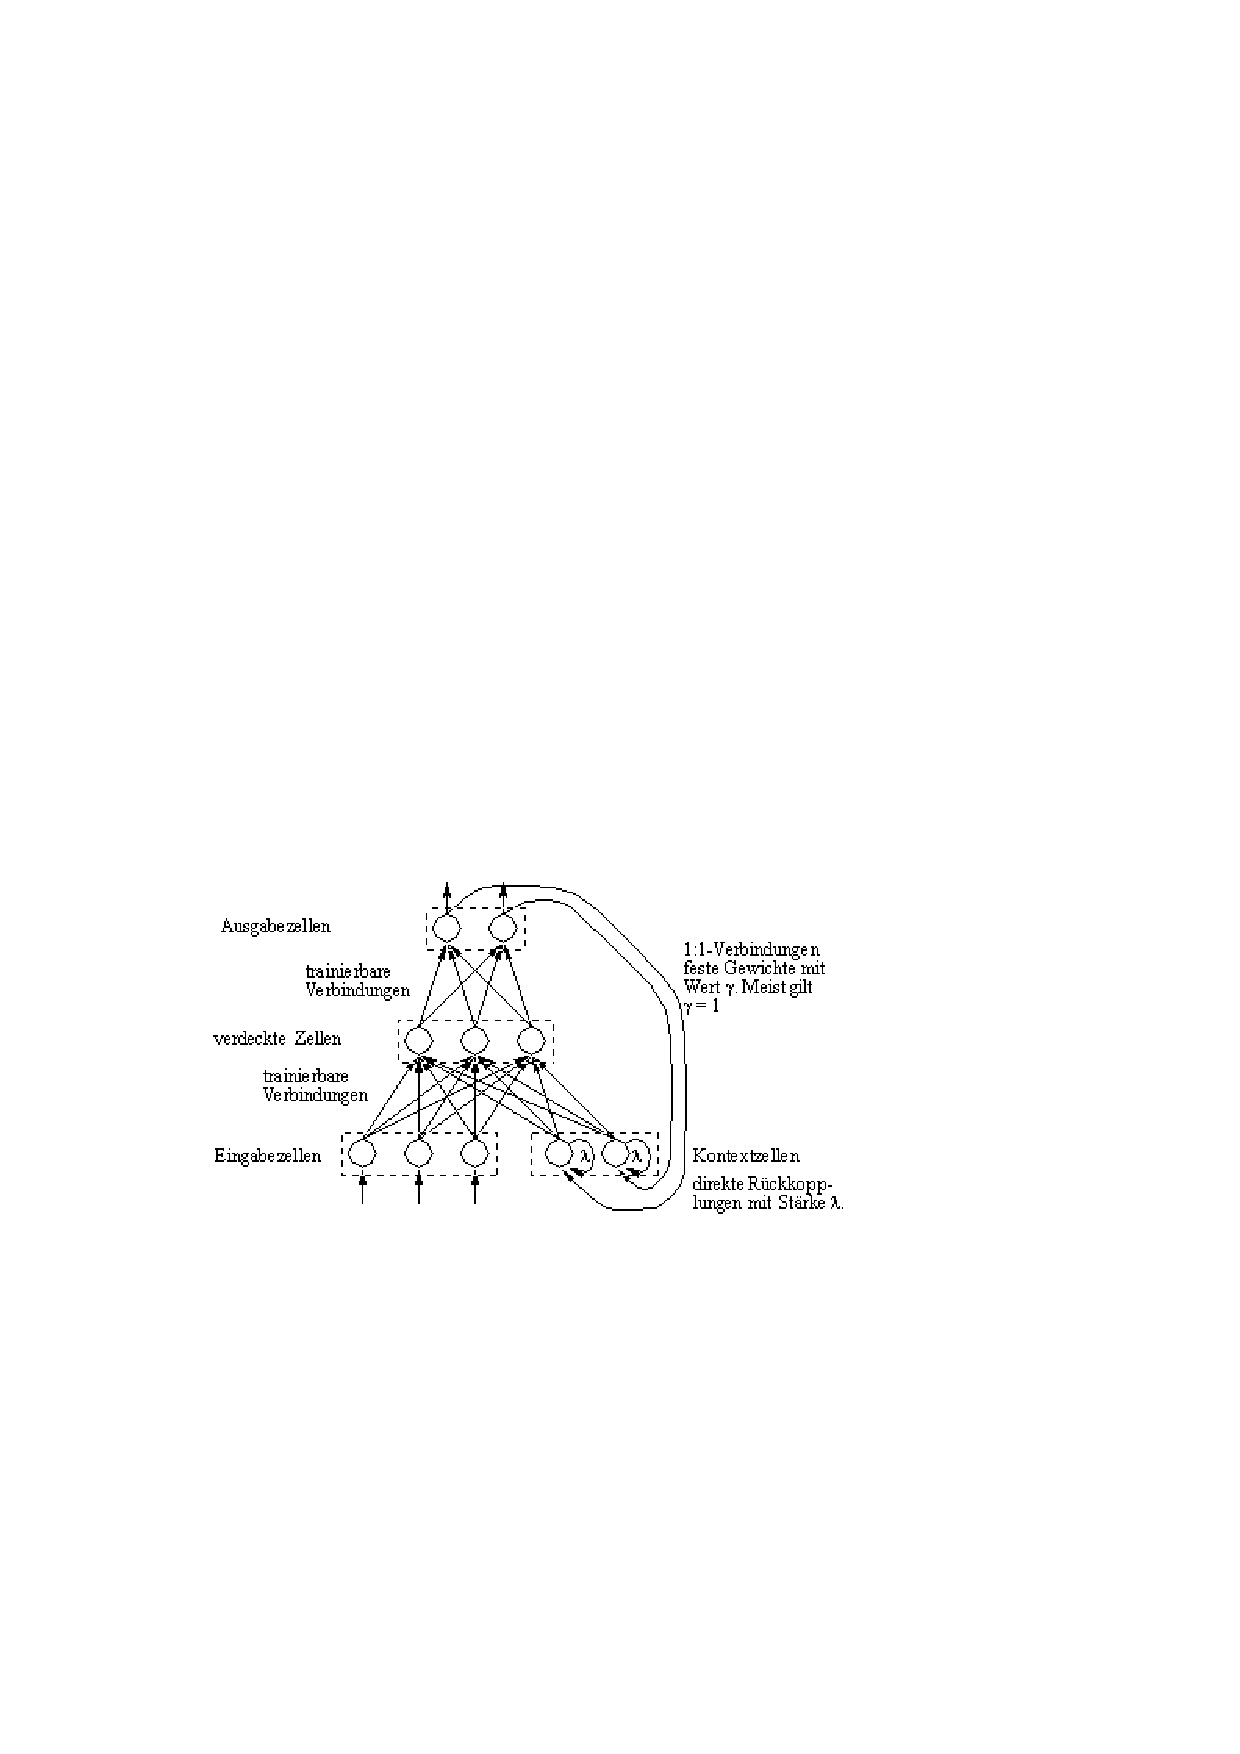
\includegraphics[width=\linewidth]{figures/ch04_jordan-netze.pdf}
	\caption{Architektur eines Jordan-Netzes.}
	\label{fig:ch04_jordan-netze}
\end{figure}

Dabei liefern die Eingabezellen zusammen mit den Kontextzellen die Netzeingabe für die Zellen der verdeckten Schicht. Deren Ausgabe wird an die Ausgabezellen weiterpropagiert und deren Ausgabe wiederum als Netzausgabe zurückgegeben und über 1:1-Rückkopplungsverbindungen mit festen Gewichten als Eingabe an die Kontextzellen weitergegeben.
Die Kontextzellen selbst besitzen direkte Rückkopplungen mit der Stärke $\lambda$, die ebenfalls fest (nicht trainierbar) sind.

Bei dieser Architektur ist zu beachten:
\begin{itemize}
	\item Die Ausgabe der \emph{Ausgabezellen} dient als Eingabe der Kontextzellen
	\item Die Zahl der Kontextzellen muss mit der Zahl der Ausgabezellen übereinstimmen.
	\item Die trainierbaren Verbindungen sind alle \emph{unidirektional}\footnote{Von der Eingabeschicht (incl. Kontextzellen) zur verdeckten Schicht und von dieser zur Ausgabeschicht.} 
\end{itemize}

Für den Fall, dass der Initialkontext der Nullvektor ist und die Rückkopplungsverbindungen von der Ausgabe zu den Kontextzellen alle den Wert $\gamma = 1$ besitzen gilt für den zeitabhängigen inneren Zustand $S(t)$:
\[
	S(t) = \sum_{n=1}^{t-1} \lambda^{n-1} O(t-n)
\]
Wobei $O(t)$ die Netzausgabe zum Zeitpunkt $t$ ist. 



% ----------------------------------------------------------------------
% ----------------------------------------------------------------------
\section*{Elman-Netze}
Elman-Netze sind eine Modifikation der Jordan-Netze, bei der die Rückkopplungsverbindungen nicht mehr von der Ausgabeschicht zur Kontextschicht, sondern von der verdeckten Schicht zur Kontextschicht verlaufen.
Weiterhin entfallen in diesem Modell die direkten Rückkopplungen der Kontextzellen zu sich selbst. Das damit entstehende Modell ist in Abbildung dargestellt.

\begin{figure}[ht!] \centering 
	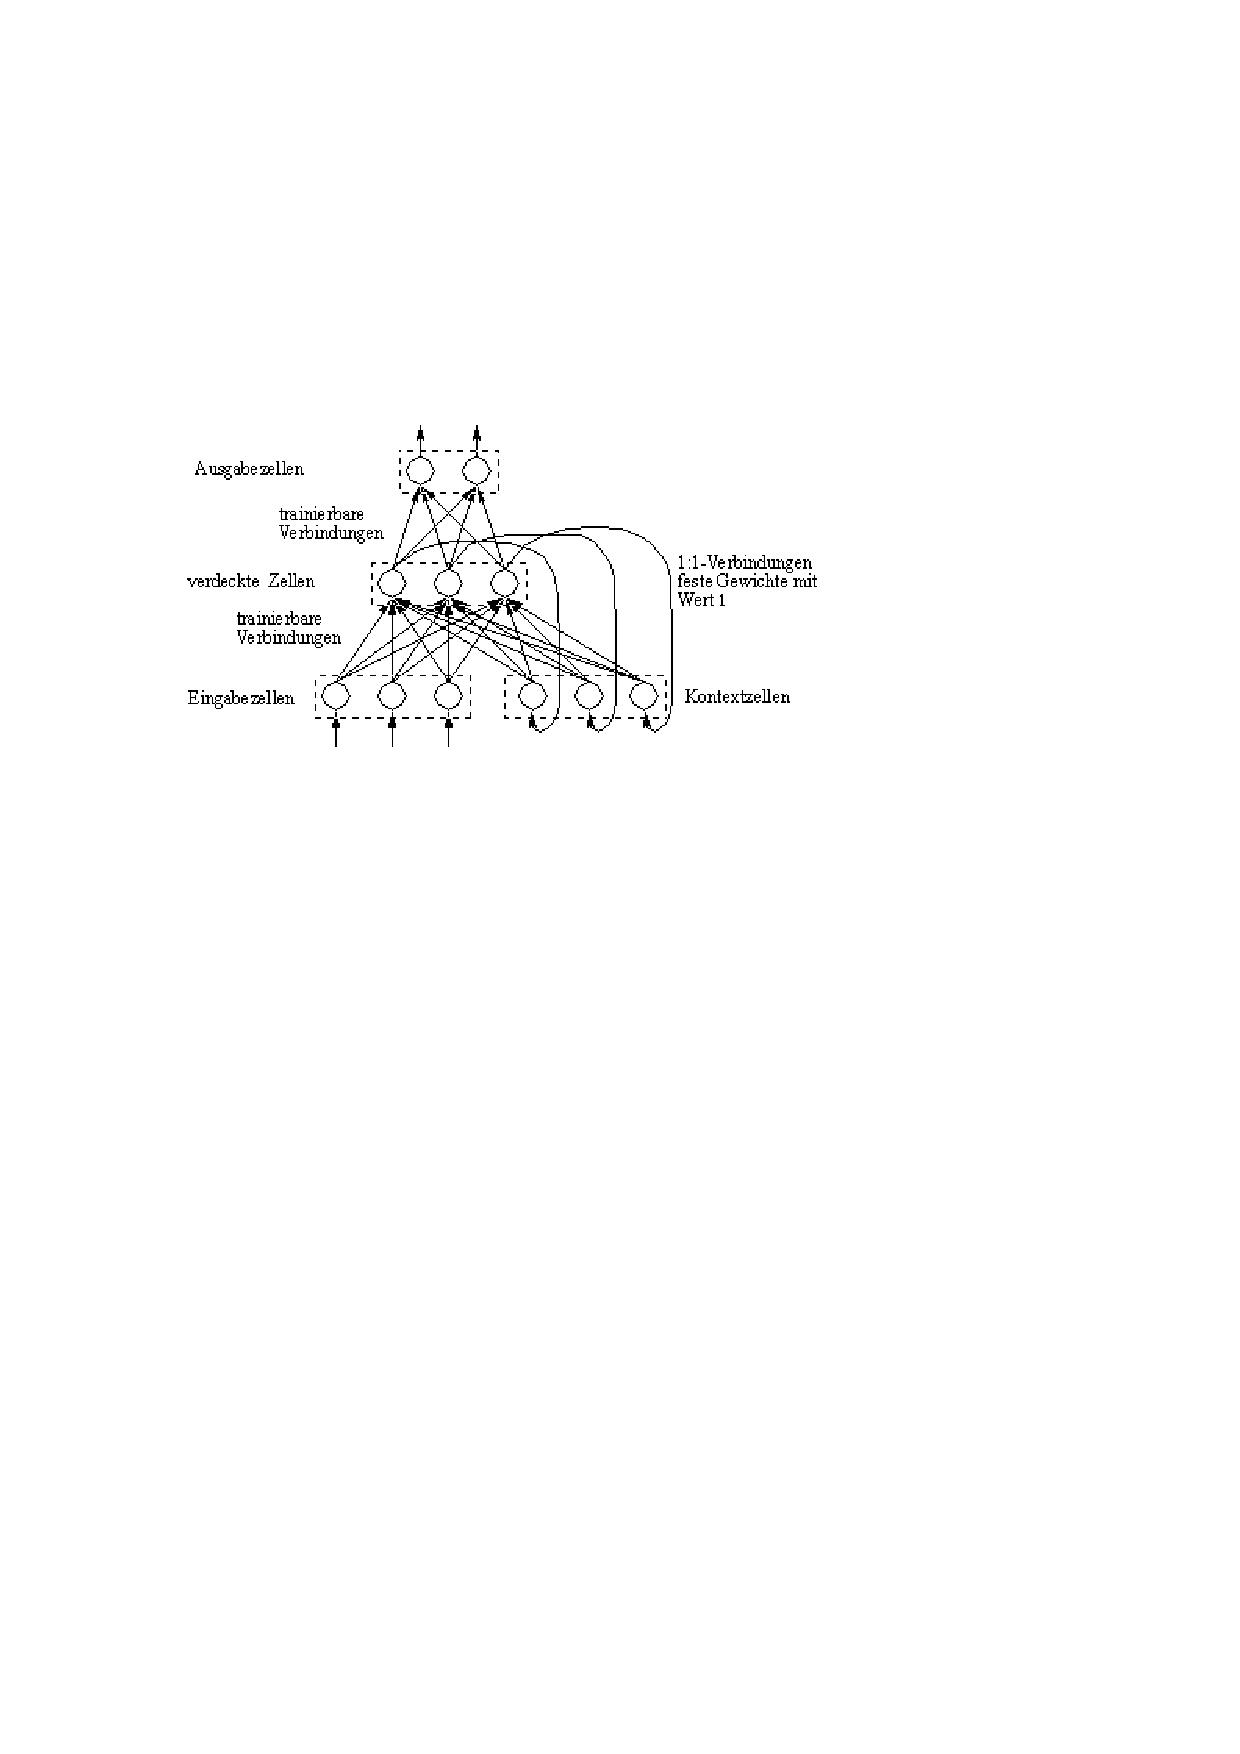
\includegraphics[width=\linewidth]{figures/ch04_elman-netze.pdf}
	\caption{Architektur eines Elman-Netzes.}
	\label{fig:ch04_elman-netze}
\end{figure}

Zu Beginn der Verarbeitung werden die Aktivierungen der Kontextzellen auf einen definierten Wert gesetzt. Nach Eingabe des ersten Musters der Musterfolge werden die verdeckten Zellen sowohl von den Eingabezellen als auch von den Kontextzellen aktiviert.
Da die Kontextzellen die Identität als Aktivierungsfunktion besitzen, ergibt sich der neue Zustand der Kontextzellen als Kopie der Ausgabe der verdeckten Zellen. 
Die verdeckten Zellen geben wie üblich ihre Ausgabe an die Ausgabezellen weiter, die ihrerseits ihre Ausgabe nach außen geben. Dies ist die gesamte Vorwärtspropagierung eines Eingabemusters.
Beim nächsten Eingabemuster enthalten allerdings die Kontextzellen die Aktivierungen der verdeckten Zellen des vorherigen Eingabemusters. Auf diese Weise kann ein zeitlicher Bezug zu früheren Mustern hergestellt werden.

Bei dieser Architektur ist zu beachten:
\begin{itemize}
	\item Die Ausgabe der \emph{versteckten Schicht} dient als Eingabe der Kontextzellen
	\item Die Zahl der Kontextzellen muss mit der Zahl der versteckten Zellen übereinstimmen.
	\item Direkte Rückkopplungen der Kontextzellen existieren nicht.
\end{itemize}

\subsection*{Elman- vs. Jordan-Netze}
Elman-Netze haben gegenüber Jordan-Netzen den Vorteil, dass die Eignung des Netzes für eine bestimmte Anwendung nicht direkt von der zu erzeugenden Ausgabesequenz abhängig ist, wie dies bei Jordan-Netzen der Fall ist. Die internen Zustände ergeben sich vielmehr aus den Zuständen der verdeckten Zellen, sodass diese direkt zu einer Repräsentation des zeitlichen Kontextes gezwungen werden.

\subsection*{Hierarchische Elman-Netze}
Die einfachen Elman-Netze besitzen nur eine verdeckte Schicht Neuronen. Für viele komplizierte Problemstellungen erzielen jedoch Netze mit mehreren verdeckten Schichten etwas bessere Ergebnisse. In diesen Fällen bieten sich hierarchische Elman-Netze an.
Eine beispielhafte Architektur ist in Abbildung \ref{fig:ch04_hierarchische-elman-netze} zu sehen.

\begin{figure}[ht!] \centering 
	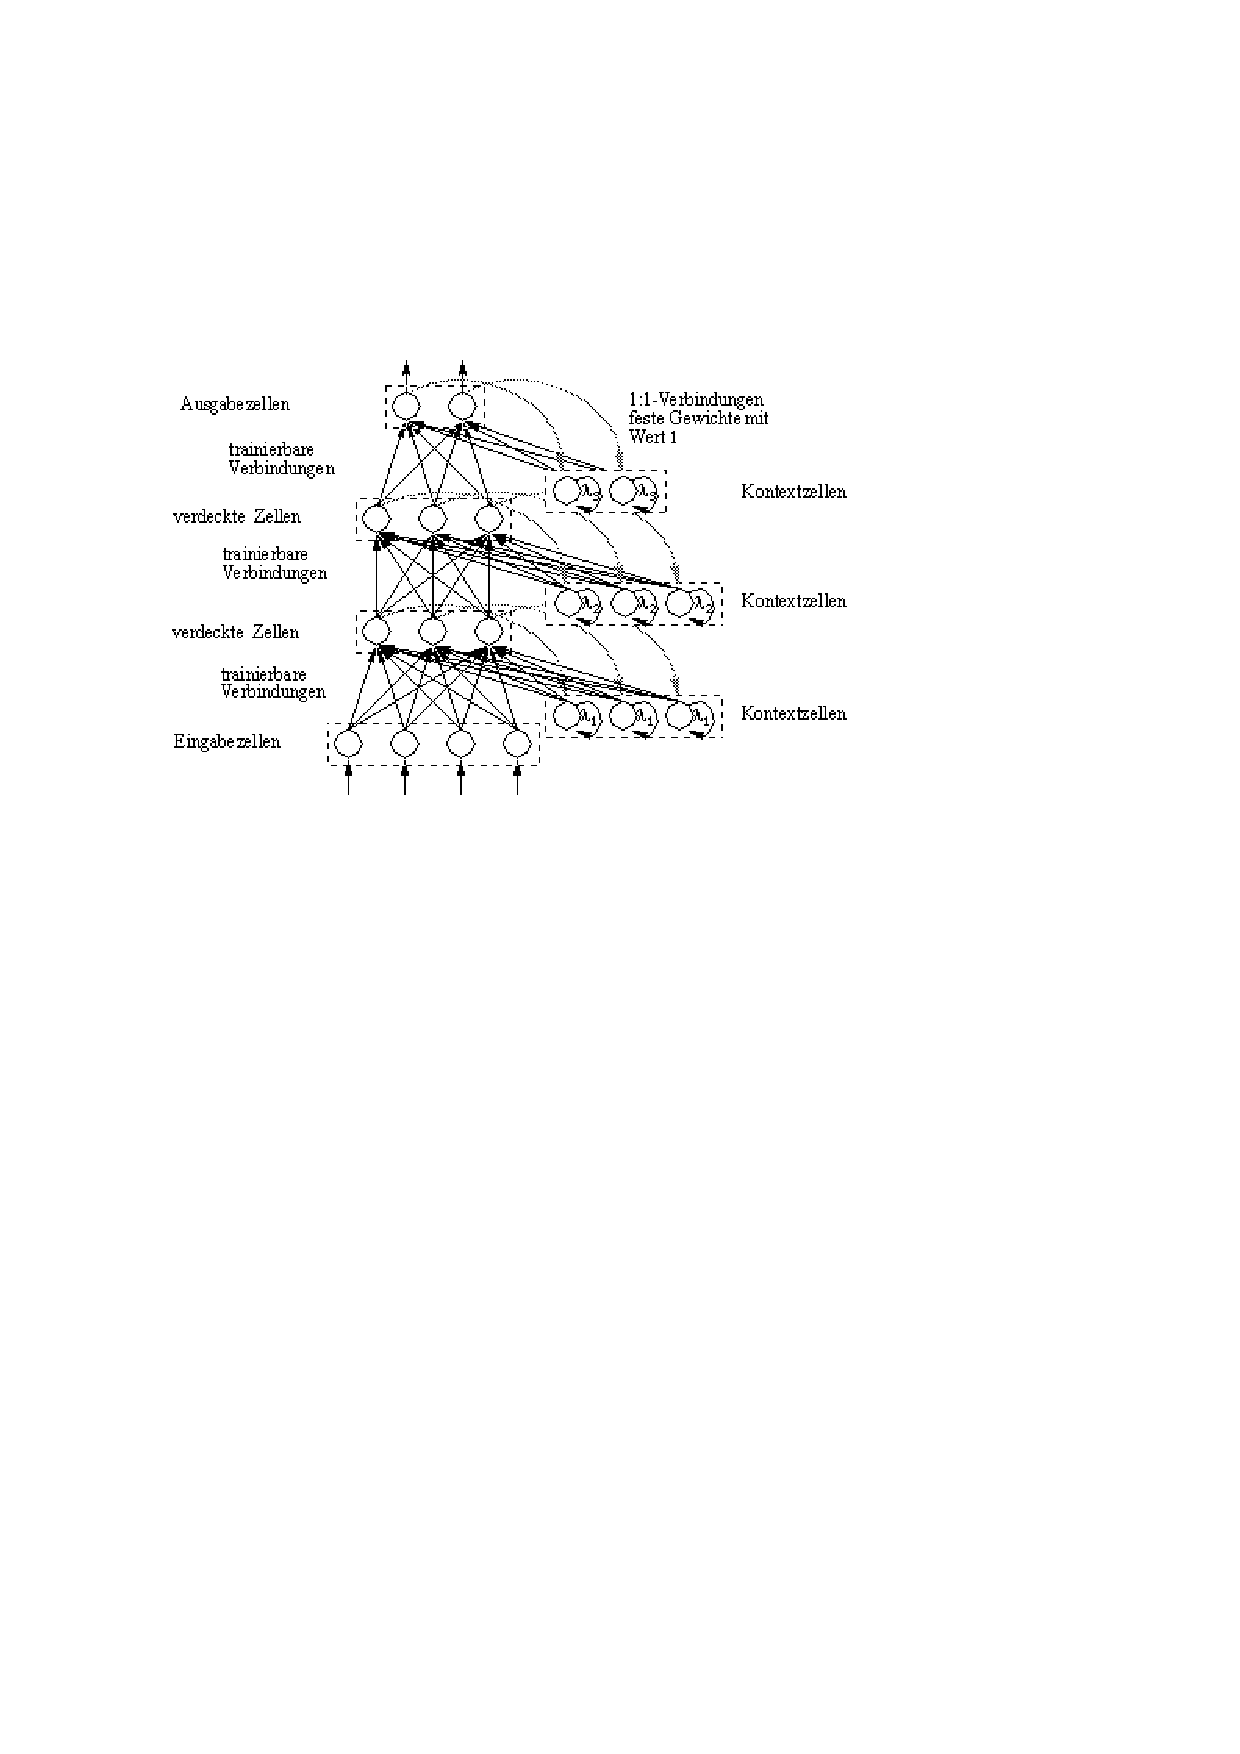
\includegraphics[width=\linewidth]{figures/ch04_hierarchische-elman-netze.pdf}
	\caption{Architektur eines Hierarchischen Elman-Netzes.}
	\label{fig:ch04_hierarchische-elman-netze}
\end{figure}

\subsubsection*{Unterschiede zu Elman-Netzen}
Die Unterschiede zu \textit{normalen} Elman-Netzen sind:
\begin{itemize}
	\item Das Netz hat mehrere verdeckte Schichten.
	\item Auch die Ausgabeschicht erhält Kontextzellen.
	\item Es existieren direkte Rückkopplungen (die Gewichte $\lambda_i$ sind nicht Null). 
\end{itemize}
Die normalen Elman-Netze stellen damit einen Sonderfall der hierarchischen Elman-Netze dar.

\subsubsection*{Vorteile}
Der Vorteil der erweiterten Elman-Netze liegt neben der Existenz mehrerer
verdeckter Schichten vor allem in der Tatsache, dass die Kontextschichten durch die Wahl unterschiedlicher Parameter $\lambda_i$ unterschiedliches Speicherverhalten haben können.



% ----------------------------------------------------------------------
% ----------------------------------------------------------------------
\section*{Lernverfahren partiell rekurrenter Netze}
Partiell rekurrente Netze können mit einer leicht abgewandelten Form des Backpropagation-Lernverfahrens oder verwandten lokalen Fehlerminimierungsverfahren (SuperSAB, Quickprop, RProp) trainiert werden.

Der Schlüssel zu ihrer Anwendung liegt in der Tatsache, dass die Übergangsfunktion, die den neuen internen Zustand beschreibt, durch die Festlegung der \emph{Gewichte der rekurrenten Verbindungen} bereits vor dem Training vollständig definiert wurde und während des Lernens nicht verändert wird.

Lässt man alle rekurrenten Verbindungen im Netz (d.h. alle Verbindungen, die zu Kontextzellen führen) weg, so reduziert sich das Netz auf ein reines feedforward-Netzwerk, bei dem die Kontextzellen einfach zusätzliche Eingabezellen sind.
Der erweiterte Eingabevektor besteht aus dem normalen Eingabevektor und dem Zustandsvektor der Kontextzellen. Der Zustandsvektor der Kontextzellen ist in jedem Schritt durch die feste Übergangsfunktion definiert. Damit kann folgende leichte Modifikation des Online-Backpropagation-Algorithmus für das Training verwendet werden.

\subsection*{Modifikation des Online-Backpropagation-Algorithmus}
Der modifizierte Backpropagation-Algorithmus für Online-Lernen ist im Folgenden aufgeführt. Die mit * markierten Schritte finden unter Nichtbeachtung der rekurrenten Verbindungen statt.

\begin{itemize}
	\item Initialisierung der Kontextzellen
	\item Für jedes Trainingsmuster aus der Musterfolge:

	\begin{itemize}
		\item \emph{Forward Propagation}: Anlegen des Eingabemusters und Vorwärtspropagierung bis zur Ausgabe*
		\item Vergleich der tatsächlichen mit der erwünschten Ausgabe und Berechnung des Fehlersignals für jede Ausgabezelle
		\item \emph{Backward Propagation}: Rückwärtsberechnung der Fehlersignale*
		\item Berechnung der Gewichtsänderung mit Hilfe der Fehlersignale
		\item Adaption der Gewichte
		\item Berechnung des Folgezustands der Kontextzellen gemäß ihrer Eingangsverbindungen (Dies ist der einzige Schritt, bei dem die rekurrenten Verbindungen beachtet werden).   
	\end{itemize}

\end{itemize}

Bei Verwendung des offline-Backpropagation-Algorithmus oder anderer Verfahren, die ein batch-Training erfordern, wie etwa Quickprop, wird der Schritt der Adaption der Gewichte aus der inneren Schleife für jedes Trainingsmuster in die äußere, hier nicht dargestellte Schleife über jede Epoche herausgezogen, sodass die Gewichte nur nach jeder Epoche adaptiert werden.




\section{Gradientenverfahren für rekurrente Netze}
% 12
% -----------------------------------------------------------------------
% -----------------------------------------------------------------------
\section*{Backpropagation Through Time (BPTT)}
Um Rekurrente Neuronale Netze (RNNs) zu trainieren gibt es mehrere Möglichkeiten. Eine der am meist verbreiteten Methoden ist \emph{Backpropagation Through Time} (BPTT).
Dabei wird das RNN in ein feed-forward Netz (FFNN) transformiert, wofür das RNN zuerst zeitlich Entfaltet (engl. unfolding in time) und anschließend mittels Backpropagation Through Time (BPTT) trainiert wird.

\subsection*{Unfolding in Time}
Nach Minsky und Papert gibt es zu jedem RNN mit diskreten Zeitschritten für eine fest vorgegebene Zeitdauer ein äquivalentes FFNN, das dieses simulieren kann.
Allerdings hat dieses FFNN extrem viele Knoten und Verbindungen. Deshalb wird dies im Folgenden am Beispiel eines kleinen rekurrenten Netzes veranschaulicht, das in Abbildung \ref{fig:ch05_einfaches-rnn} dargestellt ist.

\begin{figure}[ht!] \centering 
	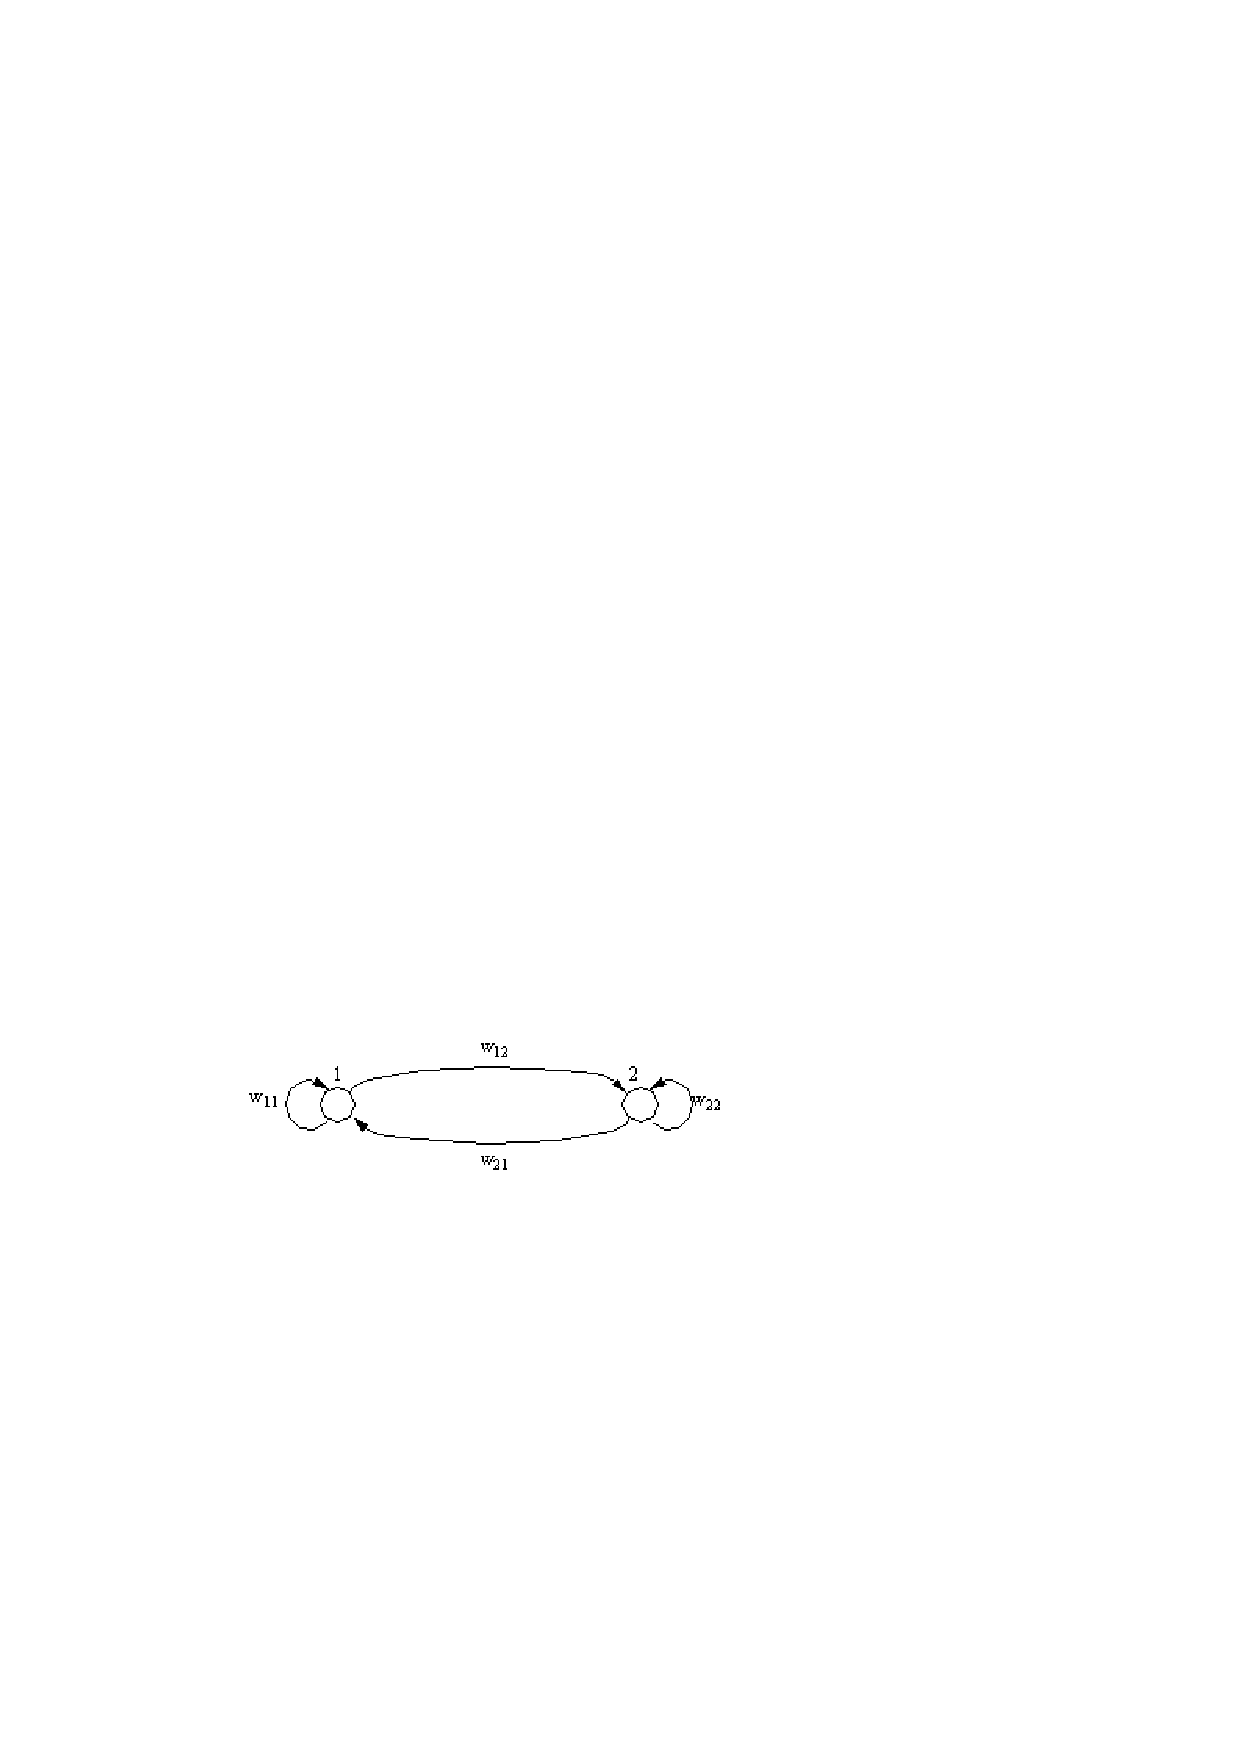
\includegraphics[width=\linewidth]{figures/ch05_einfaches-rnn.pdf}
	\caption{Einfaches RNN mit zwei Zellen.}
	\label{fig:ch05_einfaches-rnn}
\end{figure}

Durch zeitliches Entfalten werden für ein äquivalentes FFNN alle Neuronen und Gewichte des RNN für jeden diskreten Zeitschritt durch eigene Neuronen und Gewichte ersetzt. 
Dazu muss die maximale Zahl der Zeitschritte, die man untersuchen will, vorher bekannt sein. Die Verbindungsgewichte $w_{ij}$ werden dann immer von Neuron $i$ zum Zeitpunkt $t$ zu Neuron $j$ zum Zeitpunkt $t+1$ gezogen. Diese Gewichte müssen auf allen Ebenen gleich sein und den Gewichten des rekurrenten Systems entsprechen.

\begin{figure}[ht!] \centering 
	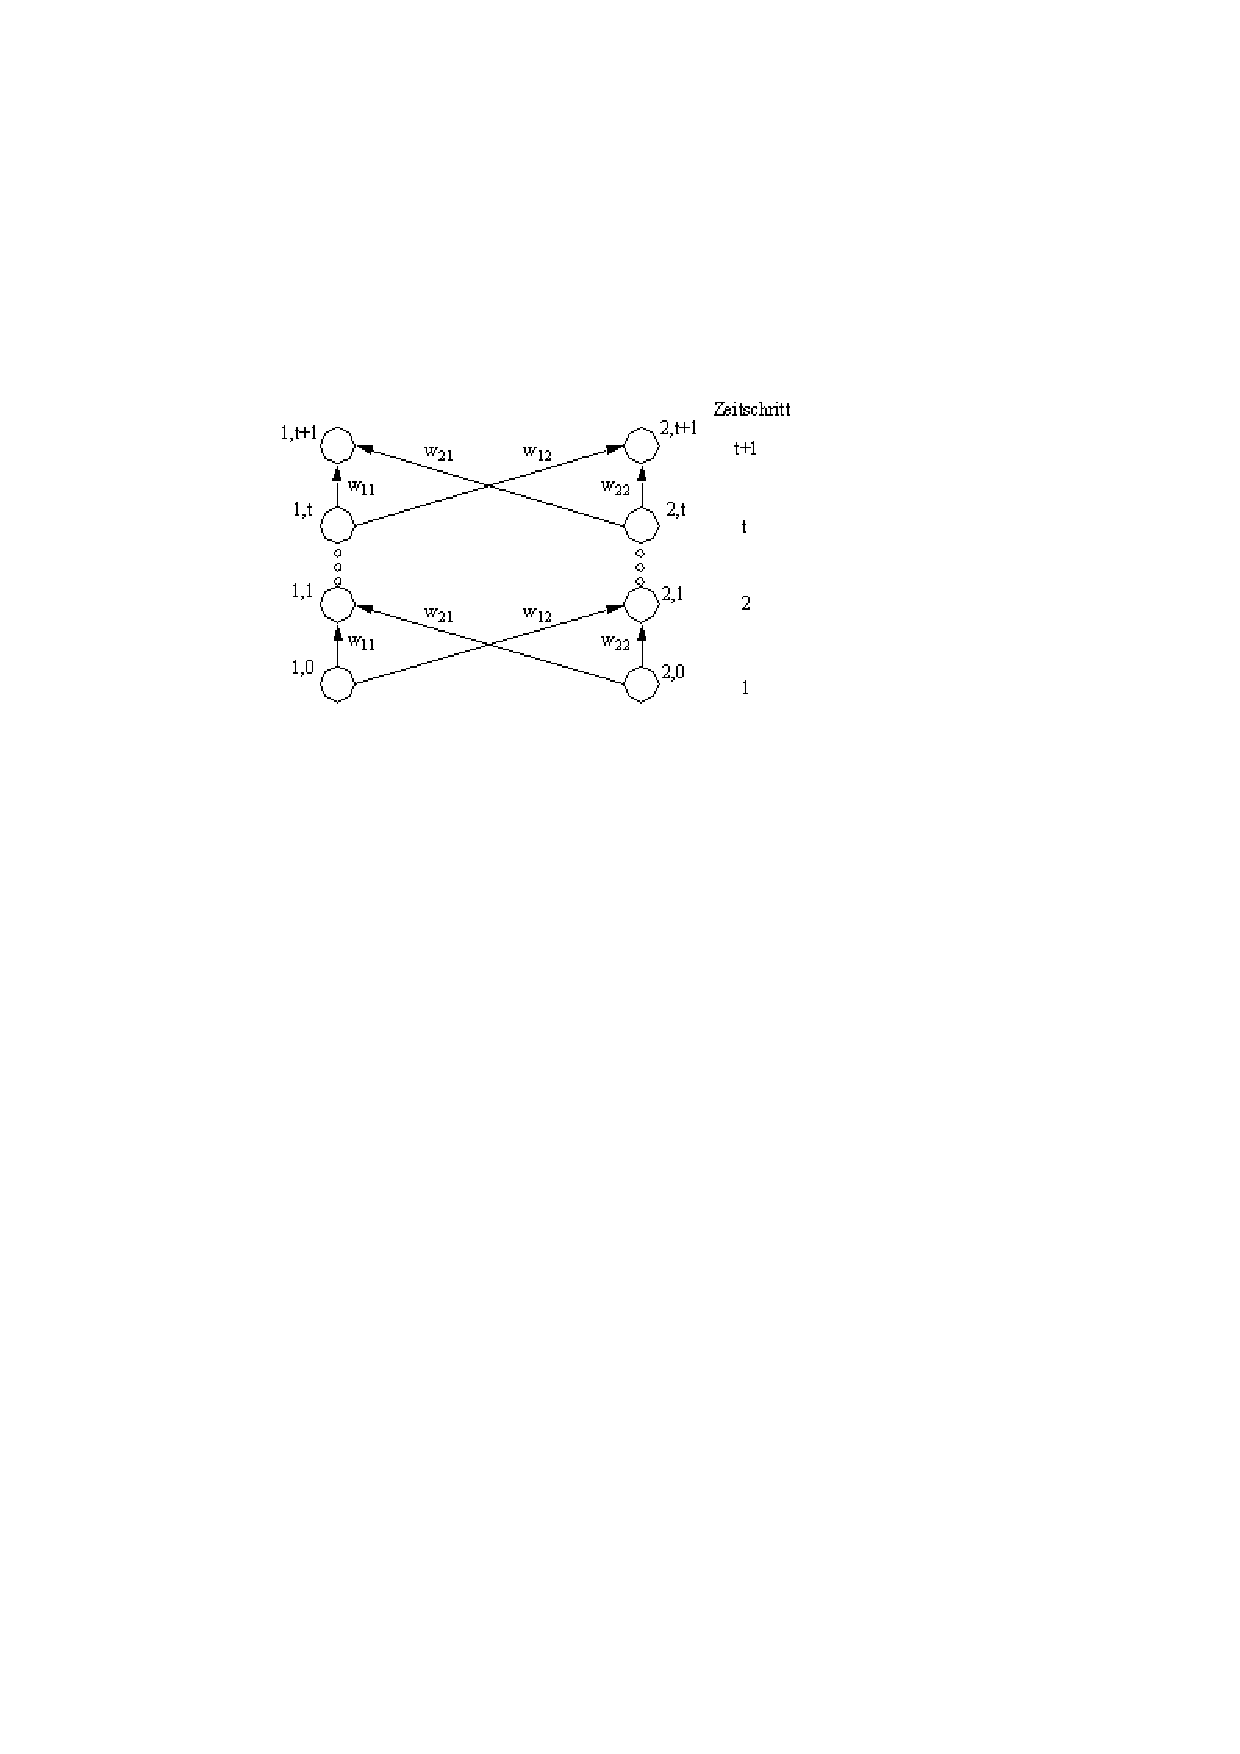
\includegraphics[width=\linewidth]{figures/ch05_ffnn-eines-rnn.pdf}
	\caption{Das zu Abbildung \ref{fig:ch05_einfaches-rnn} äquivalente FFNN.}
	\label{fig:ch05_ffnn-eines-rnn}
\end{figure}

Man sieht sofort, dass das FFNN in den Neuronen mit zweitem Index $t$ genau den Zustand anzeigt, in dem das RNN nach $t$ Zeitschritten ist. Wichtig ist hier, dass \emph{alle Gewichte mit gleichen Indizes über alle Zeitpunkte den gleichen Wert haben} (da sie ja im RNN nur als ein Gewicht vorhanden sind). Sie müssen also auch durch ein Lernverfahren alle um den gleichen Betrag geändert werden.
Mit dieser Einschränkung lässt sich dann das normale Backpropagation-Verfahren für das resultierende FFNN verwenden.

\subsection*{Weight Sharing}
Das Problem dieser Transformation ist in erster Linie der extrem hohe Speicherplatzbedarf von $O(t_{max} n^2)$ bei $n$ Neuronen und maximaler Zeitdauer $t_{max}$.

Effizienter ist eine als \emph{weight sharing} bekannte Technik, bei der die Gewichte nicht physisch vorhanden sind, sondern jeweils nur als Zeiger auf den gleichen Speicherplatz für das Gewicht. Da die Gewichte über alle Zeitschritte gleich bleiben müssen und erst nach Fehlerrückpropagierung über alle Zeitschritte um die Summe aller Änderungen geändert werden dürfen, kann man das ursprüngliche RNN, bei dem jedes Gewicht nur einmal repräsentiert war, beibehalten und sich nur die Ausgaben der Neuronen über die Zeit in einem Stapel für jedes Neuron merken. 
Dies ist in Abbildung \ref{fig:ch05_rnn-weight-sharing} dargestellt.

\begin{figure}[ht!] \centering 
	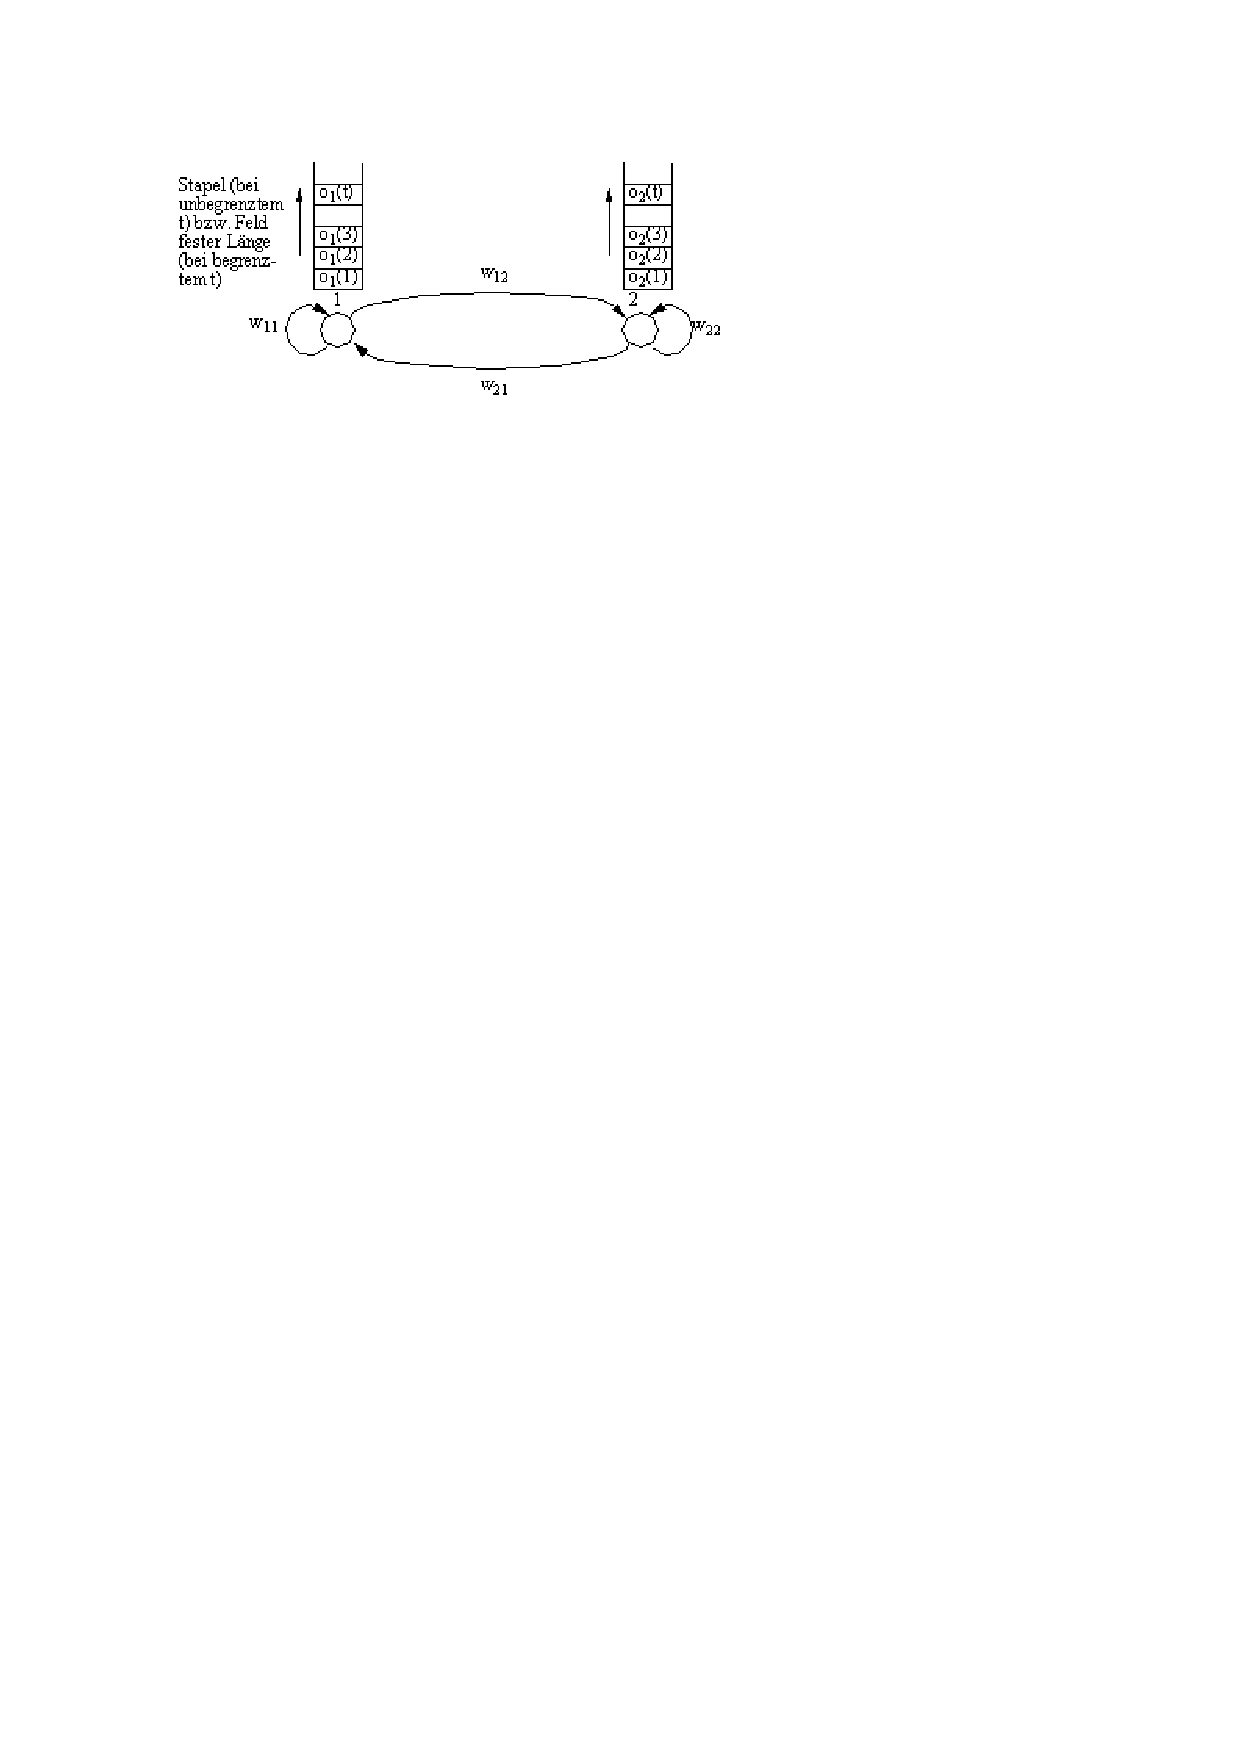
\includegraphics[width=\linewidth]{figures/ch05_rnn-weight-sharing.pdf}
	\caption{Rekurrentes Netzwerk für BPTT. Jedes Neuron besitzt einen Stapel der Ausgaben zu allen Zeitpunkten.}
	\label{fig:ch05_rnn-weight-sharing}
\end{figure}

Diese Stapel enthalten alle Ausgaben der Neuronen bis zum Zeitpunkt $t$. Neue Ausgaben werden jeweils oben auf den Stapel gelegt und nach Verwendung zur Berechnung der $\delta$-Werte für die Rückpropagierung von oben wieder gelöscht.
Da die Gewichte immer gleich bleiben sollen, brauchen sie durch weight sharing nur einmal gespeichert werden.


\subsection*{Backpropagation}
Bei rekurrenten Netzen wird üblicherweise die Eingabe (meist in Folge) angelegt, und man lässt das Netz eine Anzahl von Zyklen laufen. Zu einer bestimmten Zeit wird die Ausgabe des Netzes mit der Zielausgabe verglichen und die Fehlersignale werden für alle Ausgabeneuronen erzeugt.
Diese Fehlersignale werden dann für die gleiche Anzahl von Zyklen durch das Netz zurück propagiert. Für jede Iteration werden die Gewichtsänderungen berechnet und die Summe der Änderungen werden für jedes Gewicht gespeichert. Danach werden alle Gewichte um diese Summe geändert.

Für den Gesamtfehler $Err_p$ aller Ausgabeneuronen $k$ über die Zeit von $t=1$ bis $t=t_{max}$ gilt\footnote{In der folgenden Beschreibung wird zur besseren Übersichtlichkeit der Index $p$ für das aktuelle Muster weggelassen, die Summation über alle Muster $p$ wird an den dazu notwendigen Stellen implizit angenommen.}:
\begin{align*}
	Err_p &= \sum_{t=1}^{t_{max}} E(t)
		= \sum_{t=1}^{t_{max}} \sum_k ( E_k(t))^2 \\
	&\text{mit}\\
	E_k(t) &=
	\begin{cases}
		t_k(t) - o_k(t) &\text{falls für } k \text{ zum Zeitpunkt } t \\
			&\text{eine Ausgabe spezifiziert wurde} \\
		0	&\text{sonst}
	\end{cases}
\end{align*}
\noindent
Darüber hinaus gelten für die Gewichtsänderung $\Delta w_{ij}$ und die Fehlersignale $\delta_j$ die Zusammenhänge, welche auch beim normalen Backpropagation Algorithmus gelten:
\[
	\Delta w_{ij} = - \eta \frac{\partial E}{\partial w_{ij}}
	\quad \text{und} \quad
	\delta_j(t) = - \frac{\partial E}{\partial net_j(t)}
\]
\noindent
Für die Fehlersignale $\delta_j(t)$ gilt damit:
\begin{align*}
	\delta_j(t) = 
	\begin{cases}
		f'_{act}(net_j(t)) \cdot E_j(t) &\text{falls } t = t_{max} \\
		f'_{act}(net_j(t)) \big [ 
			E_j(t) + &\\
			\quad \sum_k \delta_k(t+1) \cdot w_{jk} \big ]
			&\text{falls } 1 \le t \le t_{max}
	\end{cases}
\end{align*}

\noindent
Daraus ergibt sich folgende Formel für die Gewichtsänderung nach Präsentation eines Musters über die gesamte Zeitdauer von $t=1$ bis $t=t_{max}$:
\[
	\Delta w_{ij} = - \eta \frac{\partial E}{\partial w_{ij}} =
		\eta \sum_{t=1}^{t_{max}} \delta_j(t) \cdot o_i(t-1)
\]

Die \emph{Zeitkomplexität} dieses Algorithmus beträgt für jeden Durchgang durch alle Zeitschritte $O(t_{max} n^2)$.

Der \emph{Speicherplatzbedarf} beträgt in dieser Realisierung nur noch $O(t_{max} n + n^2)$.

\subsection*{Fazit}
Backpropagation Through Time ist ein sehr effizientes Verfahren zum Training beliebiger rekurrenter Netze, wenn die Länge der zeitlichen Muster kleiner oder gleich der Anzahl der Neuronen des Netzwerks ist.

Für sehr lange Eingabesequenzen sind andere Verfahren, beispielsweise Real-Time Recurrent Learning (RTRL) oder die Kombination von BPTT mit RTRL von Schmidhuber besser geeignet.


\section{Cascade-Correlation}
% 13
Die \emph{Cascade-Correlation Learning Architecture} ist eine von Scott Fahlman und Christian Lebiere entwickelte Architektur Neuronaler Netze, die sich in einigen Punkten von den bisher behandelten Modellen unterscheidet: Cascade-Correlation bestimmt nicht nur die Gewichte in einem Netzwerk mit festgelegter Topologie, sondern \emph{legt die Topologie des Netzwerks
mit fest}. Es beginnt mit einem minimalen Netz und fügt während des Trainings jeweils neue verdeckte Neuronen (hidden units) einzeln hinzu.
Sobald ein neues verdecktes Neuron zum Netzwerk hinzugefügt wird, werden seine Eingangsgewichte eingefroren, so dass dieses Neuron ein Detektor für ein spezielles Teilmuster in der Eingabe bleibt.

Die Cascade-Correlation-Architektur baut damit sehr schnell Netze mit vielen Ebenen auf, die aber immer nur \emph{ein Neuron pro Ebene} besitzen.
Die Vorteile dieser Architektur sind:
\begin{itemize}
	\item Das Lernverfahren lernt Gewichte, \emph{sowie} Größe und Topologie des Netzes.
	\item Behält einmal gelernte Strukturen bei Änderung der Trainingsmenge bei (Stabilität).
	\item Keine Rückwärtspropagierung der Fehlersignale nötig.  
\end{itemize}

Es ist damit für einige Probleme sehr viel schneller als Varianten von Backpropagation.


\subsection*{Das Moving-Target-Problem}
Eines der Probleme von Backpropagation, das Anlass zur Entwicklung von Cascade-Correlation gab, war das \emph{Moving-Target-Problem}: Jedes verdeckte Neuron eines mehrstufigen feedforward-Netzes versucht beim Training gleichzeitig mit den anderen Neuronen zu einem "`nützlichen"' Detektor für ein Teilmuster (\emph{feature}) zu werden, indem es seine Eingangsgewichte entsprechend anpasst.
Diese Aufgabe wird ihm aber dadurch erschwert, dass sich alle anderen Neuronen gleichzeitig ebenfalls ändern. Die Neuronen einer verdecken Schicht können nicht direkt miteinander kommunizieren, jedes Neuron sieht nur seine eigenen Vorgängerneuronen und die von den Nachfolgeneuronen zurückpropagierten Fehler.
Dieses Fehlersignal ist das Problem, welches das einzelne Neuron zu lösen (minimieren) versucht, wobei sich aber der Fehlervektor durch die gleichzeitige Adaption aller anderen Neuronen ständig ändert. Diese gleichzeitige Änderung aller Neuronen erschwert die Anpassung für jedes einzelne Neuron.

Eine Möglichkeit, dieses Problem zu beheben, ist, nur wenige Gewichte des Netzwerks gleichzeitig zu ändern und den Rest konstant zu halten.
Cascade-Correlation verwendet ein Extrem dieser Strategie, indem es nur die Gewichte \emph{eines} Neurons zu jedem Zeitpunkt ändert.
Man könnte glauben, dass diese Strategie die Geschwindigkeit des Lernens vermindert, aber Messergebnisse zeigen, dass Cascade-Correlation damit für viele Probleme schneller lernt als die bekannten Varianten von Backpropagation.

\subsection*{Der Cascade-Correlation-Algorithmus}
Der Cascade-Correlation-Algorithmus lässt sich durch zwei Ideen charakterisieren:
\begin{enumerate}
	\item \emph{Kaskaden-Architektur} - In ihr werden verdeckte Neuronen einzeln zum Netzwerk hinzugefügt und ihre Eingangsgewichte danach nicht mehr verändert.
	\item \emph{Lernalgorithmus} - Er erzeugt die versteckten Neuronen und bestimmt deren Gewichte so, dass der Betrag der Korrelation zwischen der Ausgabe des Neurons und dem restlichen Fehlersignal maximal wird. So kann er den Restfehler möglichst stark minimieren.
\end{enumerate}

\subsubsection*{Kaskaden-Architektur}
Die Architektur eines Cascade-Correlation-Netzes ist in Abbildung \ref{fig:ch06_cascade-correlation} dargestellt.

\begin{figure}[ht!] \centering 
	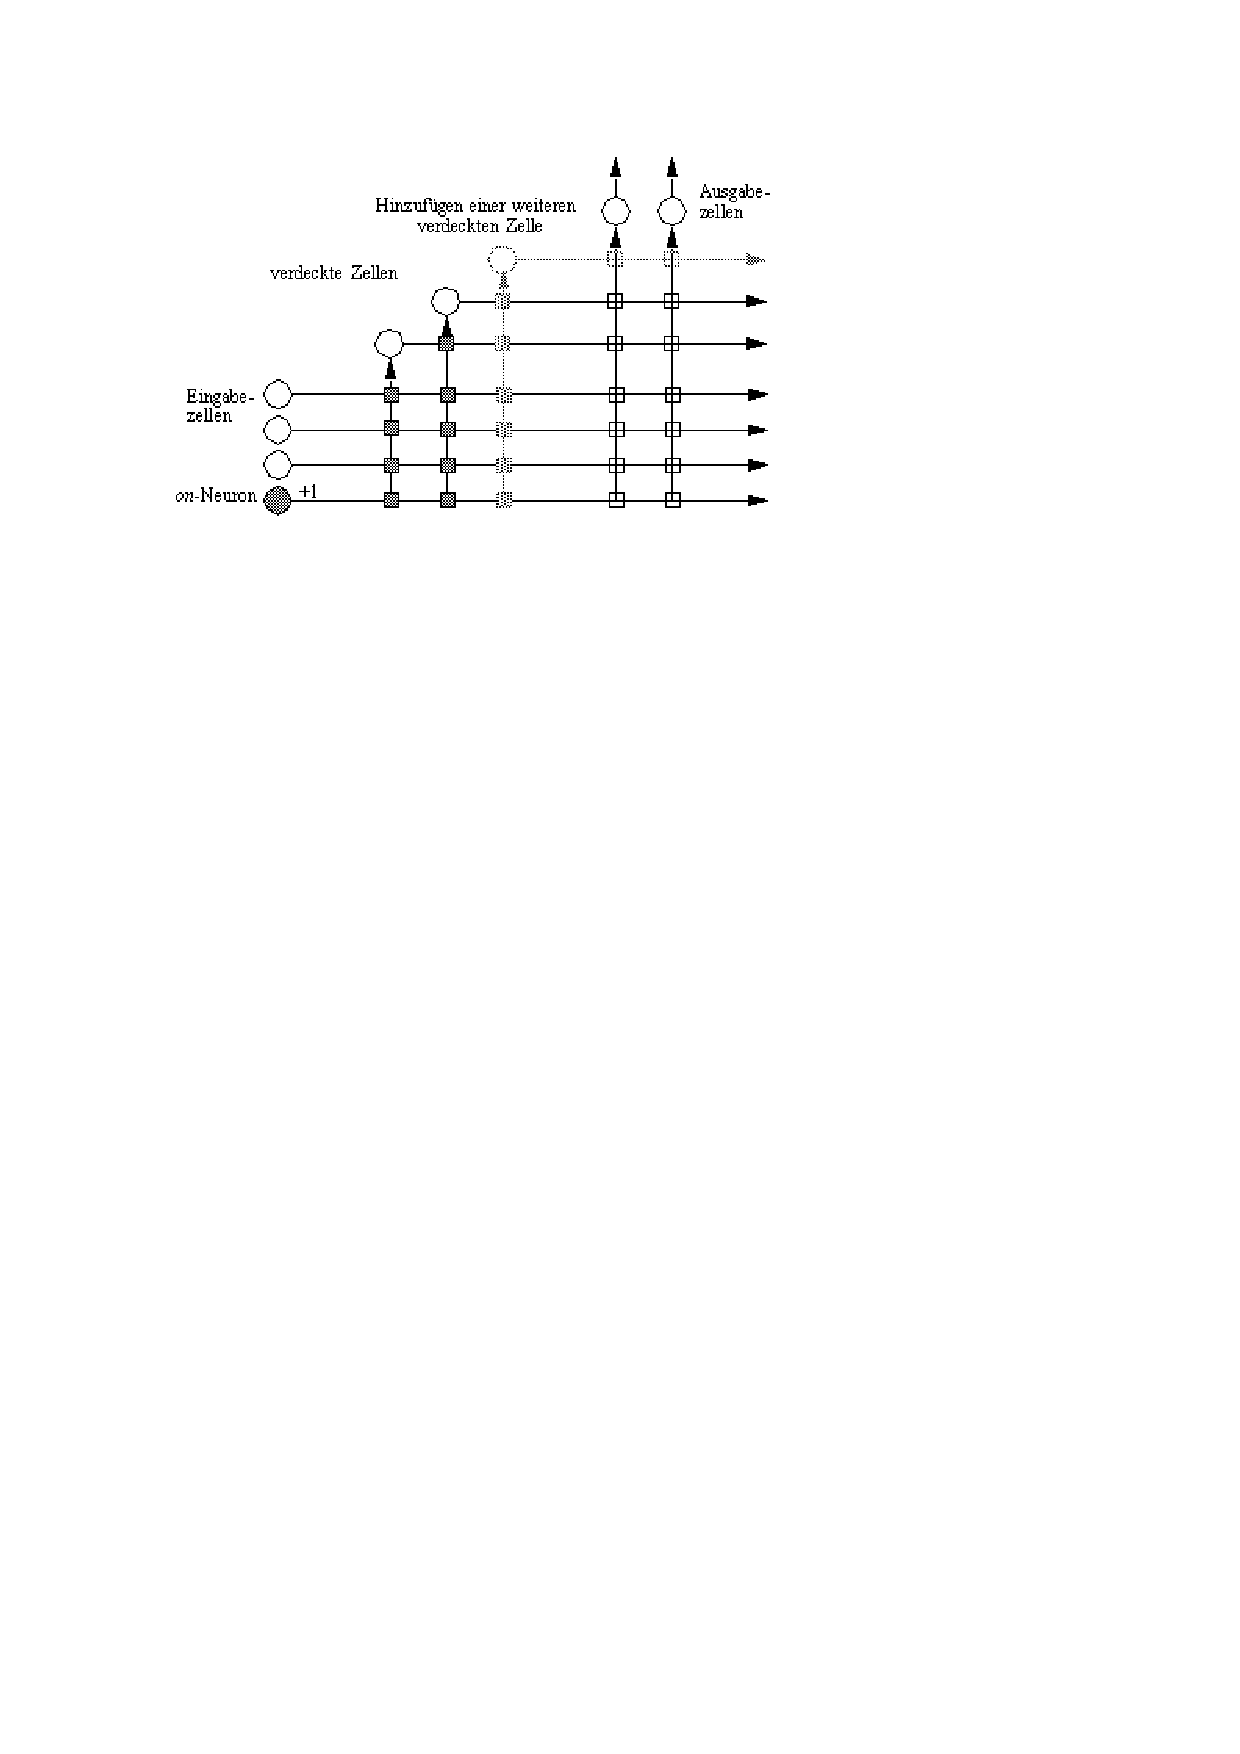
\includegraphics[width=\linewidth]{figures/ch06_cascade-correlation.pdf}
	\caption{Beispielhafte Cascade-Correlation"--Architektur, vor dem Hinzufügen des dritten verdeckten Neurons. Die vertikalen Verbindungen summieren alle Eingaben auf. Die Gewichte $w_{ij}$ sind als kleine Quadrate dargestellt. Dunkle Quadrate symbolisieren eingefrorene Gewichte, helle Quadrate sind Gewichte, die noch weiter trainiert werden.}
	\label{fig:ch06_cascade-correlation}
\end{figure}

Zu Beginn des Trainings existiert nur die durch die Problemstellung vorgegebene Anzahl von Eingabe- und Ausgabezellen, jedoch keine verdeckten Neuronen. Jede Eingabezelle ist mit jeder Ausgabezelle durch eine Verbindung mit trainierbarem Gewicht verbunden (helle Quadrate). Es existiert auch ein "`on"'-Neuron, dessen Ausgabe immer $+1$ ist und das mit allen Ausgabezellen verbunden ist, oder alternativ ein Schwellenwert in jeder dieser Zellen.
Die Ausgabeneuronen können eine lineare oder eine nichtlineare Aktivierungsfunktion besitzen\footnote{Die meisten Experimente mit Cascade-Correlation wurden bisher mit sigmoiden Aktivierungsfunktionen wie tangens hyperbolicus $tanh(x)$ oder der logistischen Aktivierungsfunktion durchgeführt.}.


\subsection*{Lernalgorithmus}
Das Lernverfahren fügt nun einzeln verdeckte Neuronen zu dem Netzwerk hinzu.
\begin{itemize}
	\item Jedes neue Neuron erhält Eingaben von \emph{allen} Vorgängern (Eingabeneuronen und vorher generierte versteckte Neuronen).
	\item Die Eingabegewichte jedes neuen Neurons werden eingefroren.
	\item Nur Gewichte zu den Ausgabeneuronen werden weiter trainiert.
\end{itemize}

Auf diese Art und Weise stellt jedes Neuron der verdeckten Schicht eine Ebene für sich dar. Dies führt zur Erzeugung sehr mächtiger Detektoren für Teilmuster höherer Ordnung, hat jedoch den Nachteil, dass das erzeugte Netzwerk recht tief ist und verdeckte Neuronen einen immer größeren "`fan-in"' erhalten.

Der Lernalgorithmus beginnt zuerst ohne verdeckte Neuronen. Die direkten Verbindungen zwischen Eingabeebene und Ausgabeebene werden über die gesamte Trainingsmenge so gut wie möglich trainiert, beispielsweise durch die Delta-Regel (Widrow-Hoff-Regel) oder durch Quickprop.

Sobald über eine Anzahl von Zyklen keine deutliche Änderung des Fehlers mehr zu beobachten ist wird das Netzwerk ein letztes Mal mit der gesamten Trainingsmenge getestet und der kumulierte Fehler gemessen. 

\begin{itemize}
	\item Ist dieser klein genug, terminiert das Verfahren ohne Erzeugung verdeckter Neuronen mit einem einstufigen Netzwerk (einer Ebene trainierter Gewichte zwischen Eingabe und Ausgabe).
	\item Im anderen Fall gibt es einen Restfehler, der durch Einführung eines oder mehrerer verdeckter Neuronen reduziert werden muss. Es wird ein neues verdecktes Neuron dem Netz hinzugefügt, dessen Gewichte der Eingangsverbindungen wie nachfolgend beschrieben bestimmt werden. \\
	Dieser Vorgang des Hinzufügens wird wiederholt, bis der Fehler klein genug ist (oder bis die maximal tolerierbare Zeit zum Training überschritten wurde).
\end{itemize}

Zur Erzeugung einer neuen verdeckten Zelle beginnt man mit einer \emph{Kandidatenzelle} $j$, die trainierbare Gewichte von allen Vorgängern erhält, während die Ausgabe noch nicht mit dem Netzwerk verbunden ist.
Nun erfolgt eine Anzahl Durchläufe durch die gesamte Trainingsmenge, wobei die Eingabegewichte wie folgt beschrieben geändert werden.

Ziel der Änderungen ist es, $S_j$, die Summe der Beträge der Korrelation\footnote{Genaugenommen ist $S$ nicht eine Korrelation, sondern eine Kovarianz, da einige Normalisierungsterme in der Formel fehlen. Tatsächlich funktioniert das Lernverfahren mit der hier angegebenen Kovarianz in den meisten Fällen sogar besser als mit der Korrelation.} zwischen $o_j$, der Ausgabe der Kandidatenzelle, und $\delta_k$,
dem Restfehler der Ausgabezelle $k$, über alle Ausgabezellen $k$ zu maximieren.
\[
	S_j = \sum_k \big | \sum_p (o_{pj} - \bar{o}_j) (\delta_{pk} - \bar{\delta_k}) \big |
\]
Dabei ist $j$ der Index der Kandidatenzelle, $k$ der Laufindex über alle Ausgabeneuronen, $p$ der Index der Muster, $\bar{o_j}$ die mittlere Ausgabe von Neuron $j$ über alle Muster $p$ und $\bar{\delta_{pk}}$ der mittlere Fehler von Ausgabezelle $k$ über alle Muster $p$.

Um $S_j$ zu maximieren, muss die partielle Ableitung $\frac{\partial S_j}{\partial w_{ij}}$ berechnet werden. Es gilt:
\[
	\frac{\partial S_j}{\partial w_{ij}} = 
		\sum_k \sum_p \sigma_k \cdot f'_{act}(net_{pj}) \cdot
		o_{pi} \cdot (\delta_{pk} - \bar{\delta{k}})
\]

Nachdem der Wert für $\frac{\partial S_j}{\partial w_{ij}}$ für jedes Gewicht von der Eingabezelle $i$ zu der Kandidatenzelle $j$ berechnet wurde, kann man einen \emph{Gradientenaufstieg} durchführen, um $S$ durch die Änderung der Verbindungsgewichte $w_{ij}$ zu maximieren.
Sobald sich $S$ nicht mehr erhöht, wird das neue verdeckte Neuron als Neuron in das aktive Netzwerk installiert, seine Eingabeverbindungen werden eingefroren und der oben beschriebene Zyklus wird fortgeführt.

Durch den Betrag in der Formel für $S_j$ versucht ein Neuron nicht das Vorzeichen, sondern nur den Betrag der Korrelation seiner Ausgabe mit dem Fehler der Ausgabeneuronen zu maximieren.
Wenn ein Neuron positiv mit dem Fehler einer Ausgabezelle korreliert, bildet es eine negative Verbindung zu dieser Ausgabezelle aus, die den Fehler vermindert; ist die Korrelation negativ, ist das Gewicht zum Ausgabeneuron positiv.

\subsubsection*{Kandidatengruppen}
Anstelle eines einzelnen Kandidatenneurons kann man auch eine Gruppe von Kandidatenneuronen trainieren\footnote{Üblich ist eine Gruppengröße von vier bis acht Kandidatenneuronen.}, jede mit einer anderen Menge von Initialgewichten. Da sie nichts miteinander zu tun haben, können alle Kandidatenneuronen \emph{parallel} trainiert werden.
Das Kandidatenneuron mit der besten Korrelation nach der Trainingsphase wird dann installiert.

Die Verwendung eine Gruppe von Kandidaten ist vorteilhaft:
\begin{itemize}
	\item Die Chance, dass ein nutzloser Kandidat, dessen Training selbst (in einem lokalen Maximum) hängen geblieben ist, permanent installiert wird, ist geringer.
	\item Das Training wird beschleunigt, weil mehrere Teile des Gewichtsraums parallel durchsucht werden können.
	\item Unterschiedliche Neuronen-Typen (z.B. sigmoid, Gauß, radial) innerhalb einer Gruppe können zu kompakteren und eleganteren Netzwerken führen.
\end{itemize}


\subsection*{Vergleich mit anderen Verfahren}
\subsubsection*{2-Spiralen-Problem}
Für den Vergleich von Cross Correlation und anderen Verfahren haben Fahlman und Lebiere das \emph{2-Spiralen-Problem} von A. Wieland genutzt.
Dieses Problem ist deshalb sehr schwer, weil durch die Verschränkung der Spirale ein feedforward-Netz mit sigmoiden Neuronen mehrere Ebenen verdeckter Neuronen und \emph{shortcut connetctions}\footnote{\emph{Shortcut connections} sind Verbindungen, welche Ebene des Netzes überspringen.} benötigt.
Abbildung \ref{fig:ch06_2-spiralen-problem} zeigt das 2-Spiralen-Problem und die von Cascade-Correlation gefundenen Separierung.

\begin{figure}[ht!] \centering 
	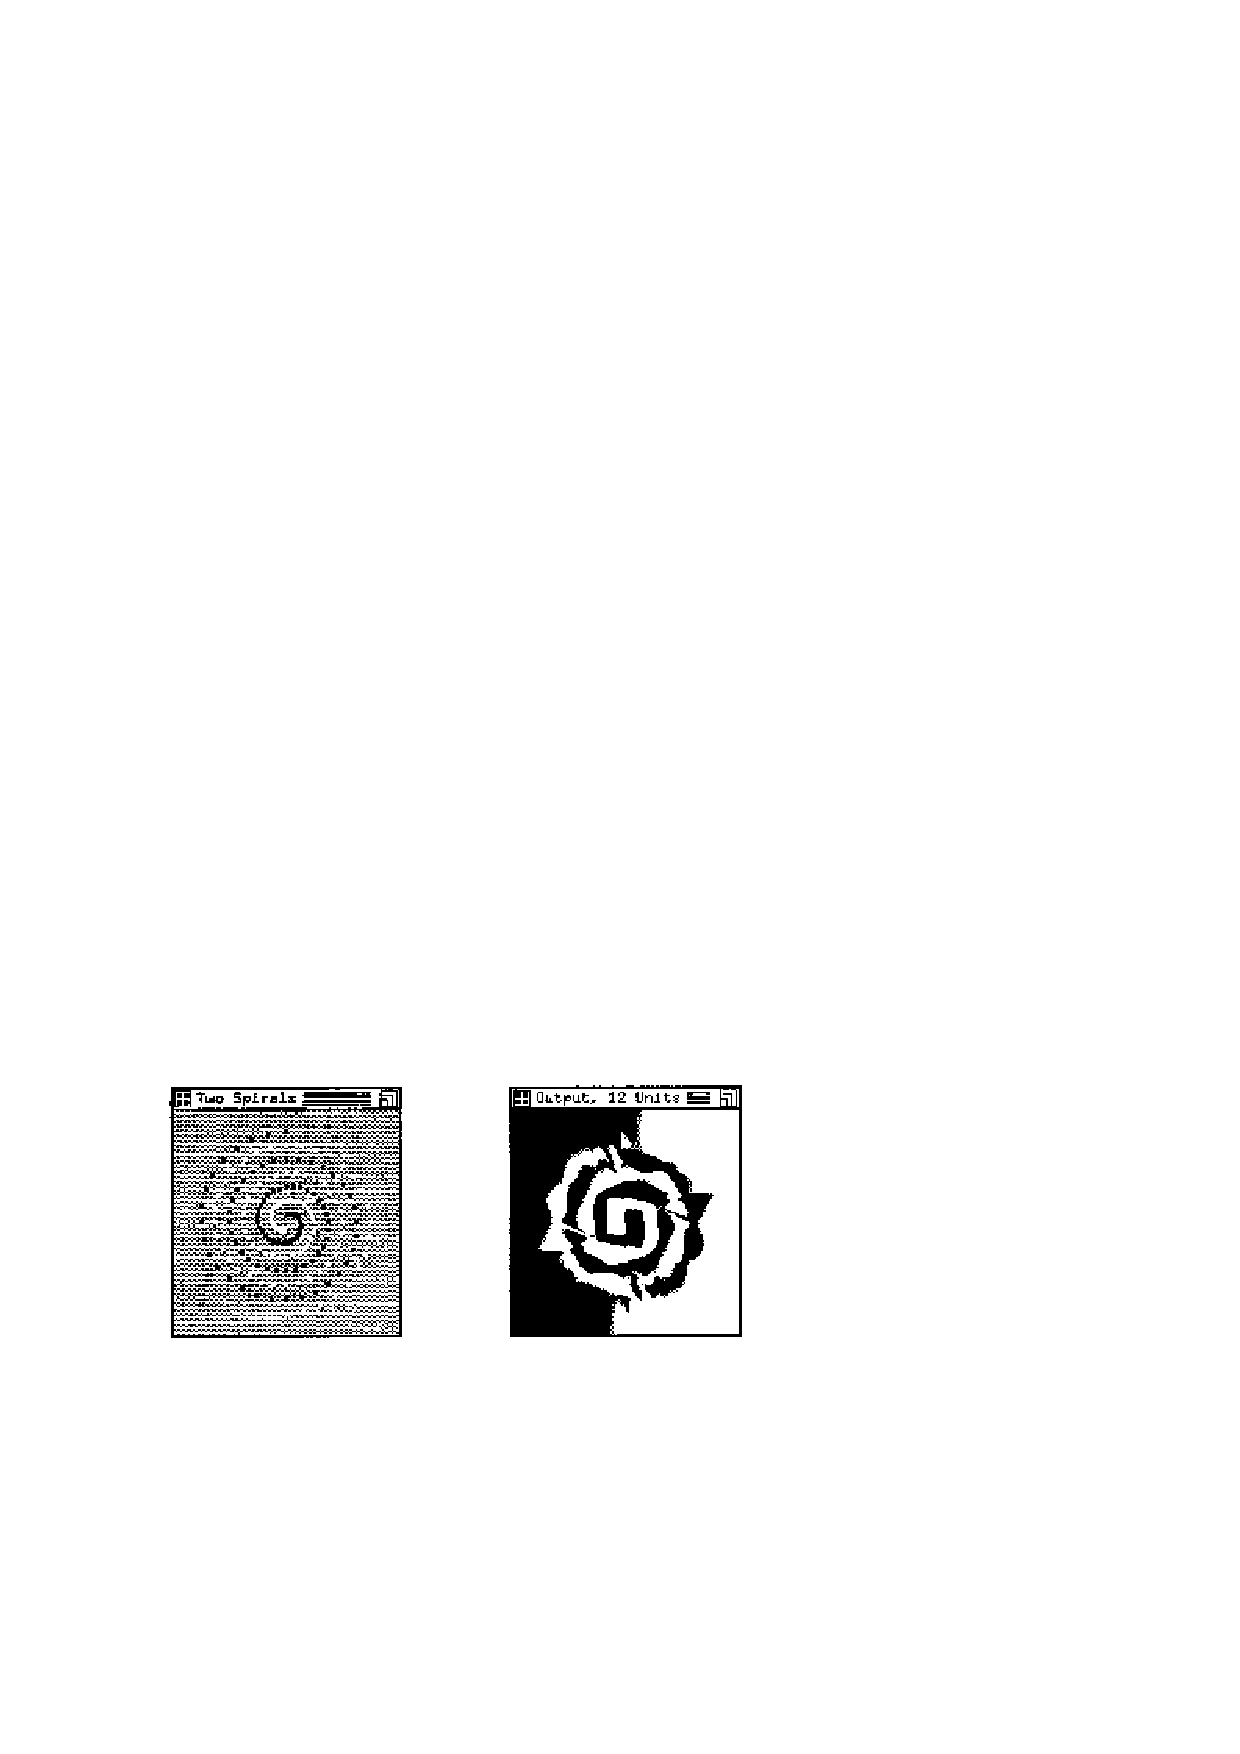
\includegraphics[width=\linewidth]{figures/ch06_2-spiralen-problem.pdf}
	\caption{Trainingspunkte des 2-Spiralen-Problems (links) und Ausgabe eines Netzwerks, das mit Cascade-Correlation trainiert wurde (rechts).}
	\label{fig:ch06_2-spiralen-problem}
\end{figure}

\subsubsection*{Ergebnisse}
Lang und Witbrock konnten mit einem 2-5-5-5-1 feedforward-Netzwerk mit shortcut connections das Problem mit Standard-Backpropagation in 20.000 Epochen lernen, Fahlman mit Backpropagation mit einer modifizierten Fehlerfunktion in 12.000 und mit Quickprop mit 8000 (etwas zeitaufwendigeren) Epochen.
Mit Cascade-Correlation mit sigmoiden Aktivierungsfunktionen und einer Gruppe von jeweils 8 Kandidatenneuronen wurden bei 100 Trainingsläufen nach Fahlman im Mittel 1700 Epochen benötigt. Dabei wurden zwischen 12 und 19 verdeckte Neuronen durch das Netz gebildet, im Mittel 15.

\subsubsection*{Geschwindigkeitsvorteil von Cascade-Correlation}
Der tatsächliche Geschwindigkeitsvorteil von Cascade-Correlation ist aus folgenden Gründen noch größer als die Faktoren 5 gegenüber Quickprop und 10 gegenüber Backpropagation aussagen:

\begin{itemize}
	\item Backpropagation und Quickprop benötigen pro Trainingszyklus eine Vorwärts- \emph{und} Rückwärtspropagierung. Cascade-Correlation nur eine Vorwärtspropagierung.
	\item Viele Trainingsepochen von Cascade-Correlation finden in den vorläufig trainierten Netzen statt, die noch nicht ihre volle Größe erreicht haben.
	\item Während die Kandidatenneuronen trainiert werden, bleiben alle Gewichte des aktiven Netzes unverändert. Daher ist es möglich, die Aktivierungen und Fehler einer ganzen Epoche abzuspeichern und die gespeicherten Werte für das Training zu verwenden, anstatt sie für jedes Trainingsmuster neu zu berechnen.
\end{itemize}

\subsection*{Eigenschaften von Cascade-Correlation}
Cascade-Correlation hat zusammenfassend betrachtet folgende Eigenschaften:

\begin{itemize}
	\item Das Verfahren findet die \emph{Topologie}\footnote{Mit \emph{Topologie} sind die Anzahl der Schichten und verdeckter Neuronen, sowie deren Verbindungen gemeint.} \emph{des Netzes} automatisch.
	\item Netze können mit \emph{unterschiedlichen Arten von Neuronen} können generiert und trainiert werden.
	\item \emph{Schnelles Lernen} (weil kein Moving-Target-Problem)
	\item Das Verfahren generiert schmale, tiefe Netze, also Detektoren höherer Ordnung für Teilmuster, \emph{ohne die dramatische Abnahme der Trainingsgeschwindigkeit}, wie sie andere Verfahren für tiefe Netze zeigen.
	\item Cascade-Correlation eignet sich für \emph{inkrementelles Lernen}, d.h. Netze können \emph{nachtrainiert} werden.\footnote{Dies ist möglich, weil einmal gelernte Detektoren nicht zerstört, aber durch Abschwächung der Gewichte zu den Ausgabeneuronen unwichtig gemacht werden können.}
	\item Weil immer nur eine Ebene von Gewichten trainiert wird, können Aktivierungen und Fehler des Netzes für mehrere Zyklen \emph{gespeichert und wiederverwendet} werden.
	\item Keine Rückpropagierung von Fehlern notwendig.
	\item Einfache Parallelisierung mehrerer Kandidaten einer Gruppe möglich.
\end{itemize}


\subsection*{Die Rekurrente Cascade-Correlation-Architektur}
Die rekurrente Cascade-Correlation-Architektur (RCC) ist eine
Variante der Cascade-Correlation-Architektur, die aus Beispielen lernen kann, \emph{eine Folge von Eingaben in eine erwünschte Folge von Ausgaben überzuführen}.
Wie in der Cascade-Correlation-Architektur werden neue Neuronen einzeln zum Netzwerk hinzugefügt. RCC behält die Vorteile von Cascade-Correlation, wie schnelles Lernen, gute Generalisierung und automatische Konstruktion kleiner, effizienter Netzwerke.

Bei rekurrenten Cascade-Correlation-Netzen kann keine vollständige Verbindung zwischen den verdeckten Neuronen realisiert werden, weil dies das Prinzip verletzen würde, dass die Eingangsgewichte einmal etablierter verdeckter Neuronen eingefroren sind und nicht mehr verändert werden können. Daher verwenden die rekurrenten Cascade-Correlation-Netze nur \emph{direkte Rückkopplungen} der verdeckten Neuronen zu sich selbst.
Dies ist in Abbildung \ref{fig:ch06_2-rcc} dargestellt.
Die rekurrente Verbindung wird gleichzeitig mit den anderen Gewichten darauf trainiert, die Korrelation des Kandidatenneurons mit dem Restfehler zu maximieren.

\begin{figure}[ht!] \centering 
	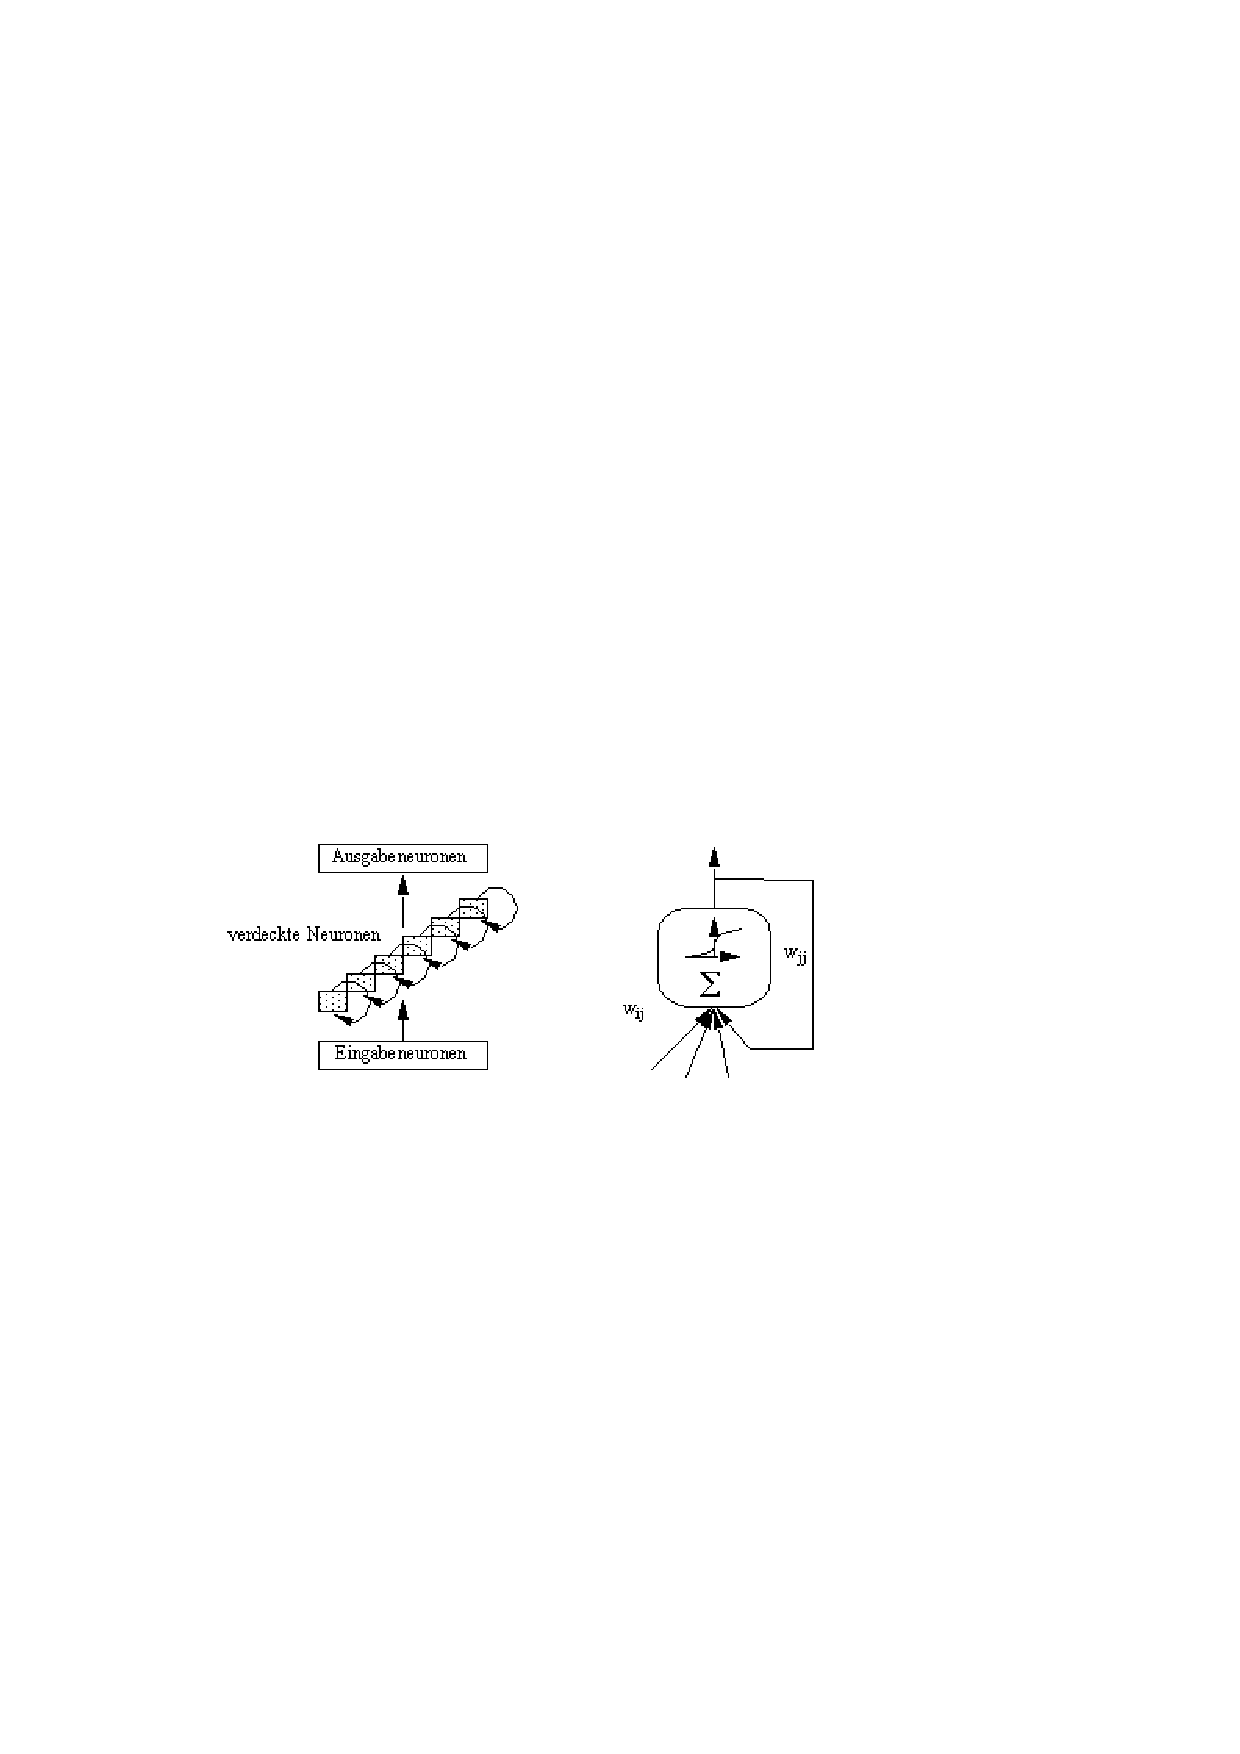
\includegraphics[width=\linewidth]{figures/ch06_rcc.pdf}
	\caption{Architektur rekurrenter Cascade-Correlation-Netze (links) und ein Kandidatenneuron $j$ mit einer rekurrenten Verbindung zu sich selbst (rechts).}
	\label{fig:ch06_2-rcc}
\end{figure}


\subsubsection*{Training}
Das Verhalten eines Kandidatenneurons mit rekurrenter Verbindung zu sich selbst ist im Folgenden aufgeführt.

\begin{itemize}
	\item \emph{stark positives} Gewicht $w_{jj}$ - Das Kandidatenneuron fungiert als Flip-Flop: Es versucht seinen Zustand beizubehalten, wenn er nicht durch eine starke Netzeingabe geändert wird.
	\item \emph{stark negatives} Gewicht $w_{jj}$ - Das Kandidatenneuron oszilliert bei jedem Zeitschritt zwischen positiver und negativer Ausgabe. 
\end{itemize}

Sobald das Kandidatenneuron dem aktiven Netzwerk hinzugefügt wird, wird sein rekurrentes Gewicht ebenso wie die anderen Eingangsverbindungen eingefroren. Auf diese Art und Weise kann jedes verdeckte Neuron als eine Zustandsvariable in einem endlichen Automaten angesehen werden, der speziell für diese Aufgabe gebaut wurde.

Fahlman verwendet meistens die Funktion $f_{act}(x) = tanh(x)$ als Aktivierungsfunktion.
Während der Trainingsphase werden alle Gewichte $w_{ij}$ so geändert, dass sie die Korrelation des Kandidatenneurons mit dem Restfehler maximieren. Dies erfordert die Berechnung der Ableitung der Ausgabe nach den Gewichten $w_{ij}$ und $w_{jj}$:
\begin{align*}
	\frac{\partial}{\partial w_{ij}} o_j(t) &= 
		f'_{act}(net_j) \Big( o_i(t) + 
			\frac{\partial}{\partial w_{ij}} o_j(t-1) w_{jj} \Big)
			\quad i \ne j \\
	\frac{\partial}{\partial w_{jj}} o_j(t) &= 
		f'_{act}(net_j) \Big( o_j(t-1) + 
			\frac{\partial}{\partial w_{jj}} o_j(t-1) w_{jj} \Big)	
\end{align*}
\noindent
Der Term ganz rechts in den Gleichungen gibt den Einfluss des betreffenden Gewichts auf den vorigen Zustand des Neurons an. Da der Wert von im vorhergehenden Schritt berechnet wurde, kann er einfach gespeichert werden und im aktuellen Schritt verwendet werden.

Damit benötigt die rekurrente Version des Verfahrens die Speicherung eines weiteren Wertes für jedes Gewicht und der alten Aktivierung $o_j(t-1)$ des Neurons. Zum Zeitpunkt $t=0$ werden die Ausgaben der Neuronen und alle partiellen Ableitungen als Null angenommen.

In den Benchmarks zeigte sich, dass RCC für die untersuchten Aufgaben leistungsfähiger als Standard-Elman-Netze war, während sich RTRL als etwa gleich leistungsfähig im Vergleich, aber komplexer und für größere Netze als weniger gut geeignet herausstellte.



\section{Lernende Vektorquantisierung LVQ}
% 14
% ----------------------------------------------------------------------
% ----------------------------------------------------------------------
\section*{Quantisierung}
Unter \emph{Quantisierung} (auch \emph{Diskretisierung}) versteht man die Unterteilung eines kontinuierlichen Raums in diskrete Abschnitte.

Indem man der reellen Zahl $2.71828$ beispielsweise alle Nachkommastellen entfernt, könnte man diese Zahl der natürlichen Zahl $2$ zuweisen. Hierbei ist klar, dass jede andere Zahl mit einer $2$ vor dem Komma ebenfalls der natürlichen Zahl $2$ zugewiesen würde. Die $2$ wäre also eine Art \emph{Repräsentant} für alle reellen Zahlen im Intervall $[2; 3)$.

Zu beachten ist, dass wir einen Raum auch unregelmäßig quantisieren können: So wäre der Zeitstrahl einer Woche beispielsweise in Arbeitstage und Wochenende quantisierbar.

\subsection*{Spezialfall: Digitalisierung}
Ein Spezialfall der Quantisierung ist die Digitalisierung: Im Fall der Digitalisierung sprechen wir immer von einer gleich"-mäßigen Quantisierung eines kontinuierlichen Raums in ein Zahlensystem zu einer bestimmten Basis.



% ----------------------------------------------------------------------
% ----------------------------------------------------------------------
\section*{Idee von LVQ}
LVQ beschreibt eine Gruppe von \emph{überwachten} Lernalgorithmen (LVQ1, LVQ2, LVQ3 und OLVQ) und basiert auf der Vektorquantisierung (VQ), einem unüberwachten Clustering- und Lernalgorithmus.

\subsection*{Vektorquantisierung (VQ)}
Ziel der Vektorquantisierung ist es, den Merkmalsraum mit einer geringen Anzahl an Vektoren zu approximieren.
Hierfür wird eine Menge von Merkmalsvektoren $x$ zu $M$ Klassen zugeordnet. Jede dieser Klassen hat einen \emph{Prototypvektor}. Die Menge aller Prototypvektoren wird als \emph{Codebook} bezeichnet (weshalb die Prototypvektoren auch als Codebookvektoren bezeichnet werden).
Ein Merkmalsvektor $x$ wird derjenigen Klasse zugeordnet, zu welcher der Abstand zwischen Merkmalsvektor und Prototypvektor am kleinsten ist.

\begin{figure}[ht!] \centering 
	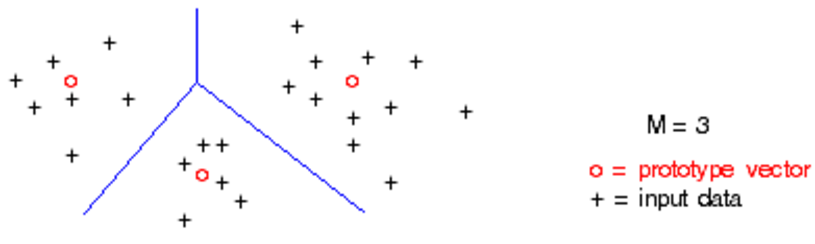
\includegraphics[width=\linewidth]{figures/ch07_vq.pdf}
	\caption{Merkmalsraum als Voronoidiagram: Dargestellt sind die $M=3$ mit $o$ gekennzeichneten Prototypvektoren und die daraus resultierenden Clustergrenzen.}
	\label{fig:ch07_vq}
\end{figure}

\subsection*{Überwachte Vektorquantisierung}
Learning Vector Quantization (LVQ) unterteilt, wie auch VQ, einen Eingaberaum durch eine Menge von Prototypvektoren in Klassen, welche den Eingaberaum möglichst gut wiedergeben. Jedes Element des Eingaberaums soll also einem solchen Vektor (nämlich dem am nächst gelegenen) zugeordnet werden können.
So wird der Eingaberaum in ein \emph{Voronoidiagramm} und damit auch in die besagten diskreten Bereiche unterteilt (siehe Abbildung \ref{fig:ch07_vq}).

Wichtig dabei ist, dass im Voraus die \emph{Anzahl der Klassen}, sowie die \emph{Klassenzugehörigkeit} eines jeden Trainingsbeispiels bekannt sein müssen. Die Klassen müssen dabei nicht disjunkt sein, sie dürfen sich also überlappen.

LVQ arbeitet mit \emph{einschichtigen} Neuronalen Netzen\footnote{Einschichtige NN sind Netze, die aus einer Schicht \emph{aktiver} Neuronen (evtl. mit vorgeschalteten Eingabeneuronen ohne Informationsverarbeitung) bestehen. Diese Neuronen werden oft als \emph{Kohonen-Neuronen} bezeichnet.} und passt die zufällig initialisierten Codebookvektoren durch Trainingsbeispiele so an, dass sie die Trainingsdaten möglichst gut widerspiegeln.



% ----------------------------------------------------------------------
% ----------------------------------------------------------------------
\section*{Training}
Für das Training von LVQ existiert eine Trainingsmenge $P$ mit $|P|$ Trainingsbeispielen, sowie eine Klassenmenge $C$ mit $|C|$ Klassen. Jeder dieser Klassen ist ein Codebookvektor eindeutig zugeordnet. Die Klassenmenge enthält damit $|C|$ Codebookvektoren $C_1, C_2, \ldots, C_{|C|}$.
\begin{hint}{Hinweis!}{lvq-training}
	Möglicherweise können auch mehrere Codebookvektoren für eine Klasse existieren. Das konnte ich nicht genau herausfinden.
	\begin{flushright}\textit{Beni}\end{flushright}
\end{hint}

\begin{hint}{Hinweis!}{prototypvektoren}
	In den folgenden Abbildungen wird ein Eingabemuster anstelle von $p$ mit $X$ und ein Prototypvektor anstelle von $C_i$ mit $W_i$ bezeichnet.
\end{hint}

Die Trainingsbeispiele sind von der Form $(p,c)$. Dabei ist $p \in P$ ein Trainingsmuster und $c \in \{1,2, \ldots, |C|\}$ dessen Klassenzugehörigkeit.

Das LVQ-Lernverfahren besteht grundsätzlich aus den folgenden Schritten:
\begin{itemize}
	\item \emph{Initialisierung} - Die $|C|$ Codebookvektoren werden zufällig im Eingaberaum platziert.
	\item \emph{Trainingsbeispiel} - Ein Trainingsbeispiel $p$ aus der Trainingsmenge $P$ wird gewählt und präsentiert.
	\item \emph{Abstandsmessung} - Der Abstand $||p - C_i||$ aller Codebookvektoren zur Trainingseingabe $p$ wird gemessen.
	\item \emph{Gewinner} - Derjenige Codebookvektor gewinnt, für den gilt:
	\begin{align*}
		\underset{C_i \in C}{min} ||p - C_i||		
	\end{align*}
	\item \emph{Lernvorgang} - Der Lernvorgang findet durch die folgenden Regeln statt:
	\begin{align*}
		\Delta C_i &= \eta(t) \cdot h(p, C_i) \cdot (p-C_i) \\
		C_i(t+1) &= C_i(t) + \Delta C_i
	\end{align*}
	Dabei ist $\eta$, wie gewohnt, die Lernrate und $(p-C_i)$ die Richtung, in die der Codebookvektor verschoben wird.
	Für das Kernstück, die Funktion $h(p, C_i)$, wird eine Fallunterscheidung vorgenommen.
	\begin{itemize}
		\item \emph{Zuweisung richtig} - Der Gewinnervektor ist der Codebookvektor der $p$ zugehörigen Klasse.\\
		In diesem Fall liefert die Funktion $h(p, C_i)$ positive Werte, der Codebookvektor bewegt sich \emph{auf $p$ zu}.
		\item \emph{Zuweisung falsch} - Der Gewinnervektor repräsentiert nicht die Klasse, der $p$ zugehörig ist.\\
		Der Gewinnervektor bewegt sich \emph{von $p$ weg}.
	\end{itemize}
\end{itemize}

Die Funktion $h$ wurde an dieser Stelle nicht genau definiert. Sie unterscheidet sich bei den, im Folgenden aufgeführten Varianten von LVQ: LVQ1, LVQ2, LVQ3, OLVQ.


% ----------------------------------------------------------------------
% ----------------------------------------------------------------------
\section*{LVQ1}
Bei LVQ1 gilt für $h$:
\begin{align*}
	h(p, C_i) =
	\begin{cases}
		+1 \quad \text{wenn } Klasse(C_i) = Klasse(p) \\
		-1 \quad \text{wenn } Klasse(C_i) \ne Klasse(p) \\
	\end{cases}
\end{align*}
\noindent
Die Lernrate $\eta(t)$ kann konstant sein oder mit der Zeit monoton fallen, um Konvergenz zu erzwingen. Es gilt jedoch: $0 < \eta(t) < 1$.
Die Adaption der Prototypvektoren wird in Abbildung \ref{fig:ch07_lvq1} grafisch veranschaulicht.

\begin{figure}[ht!] \centering 
	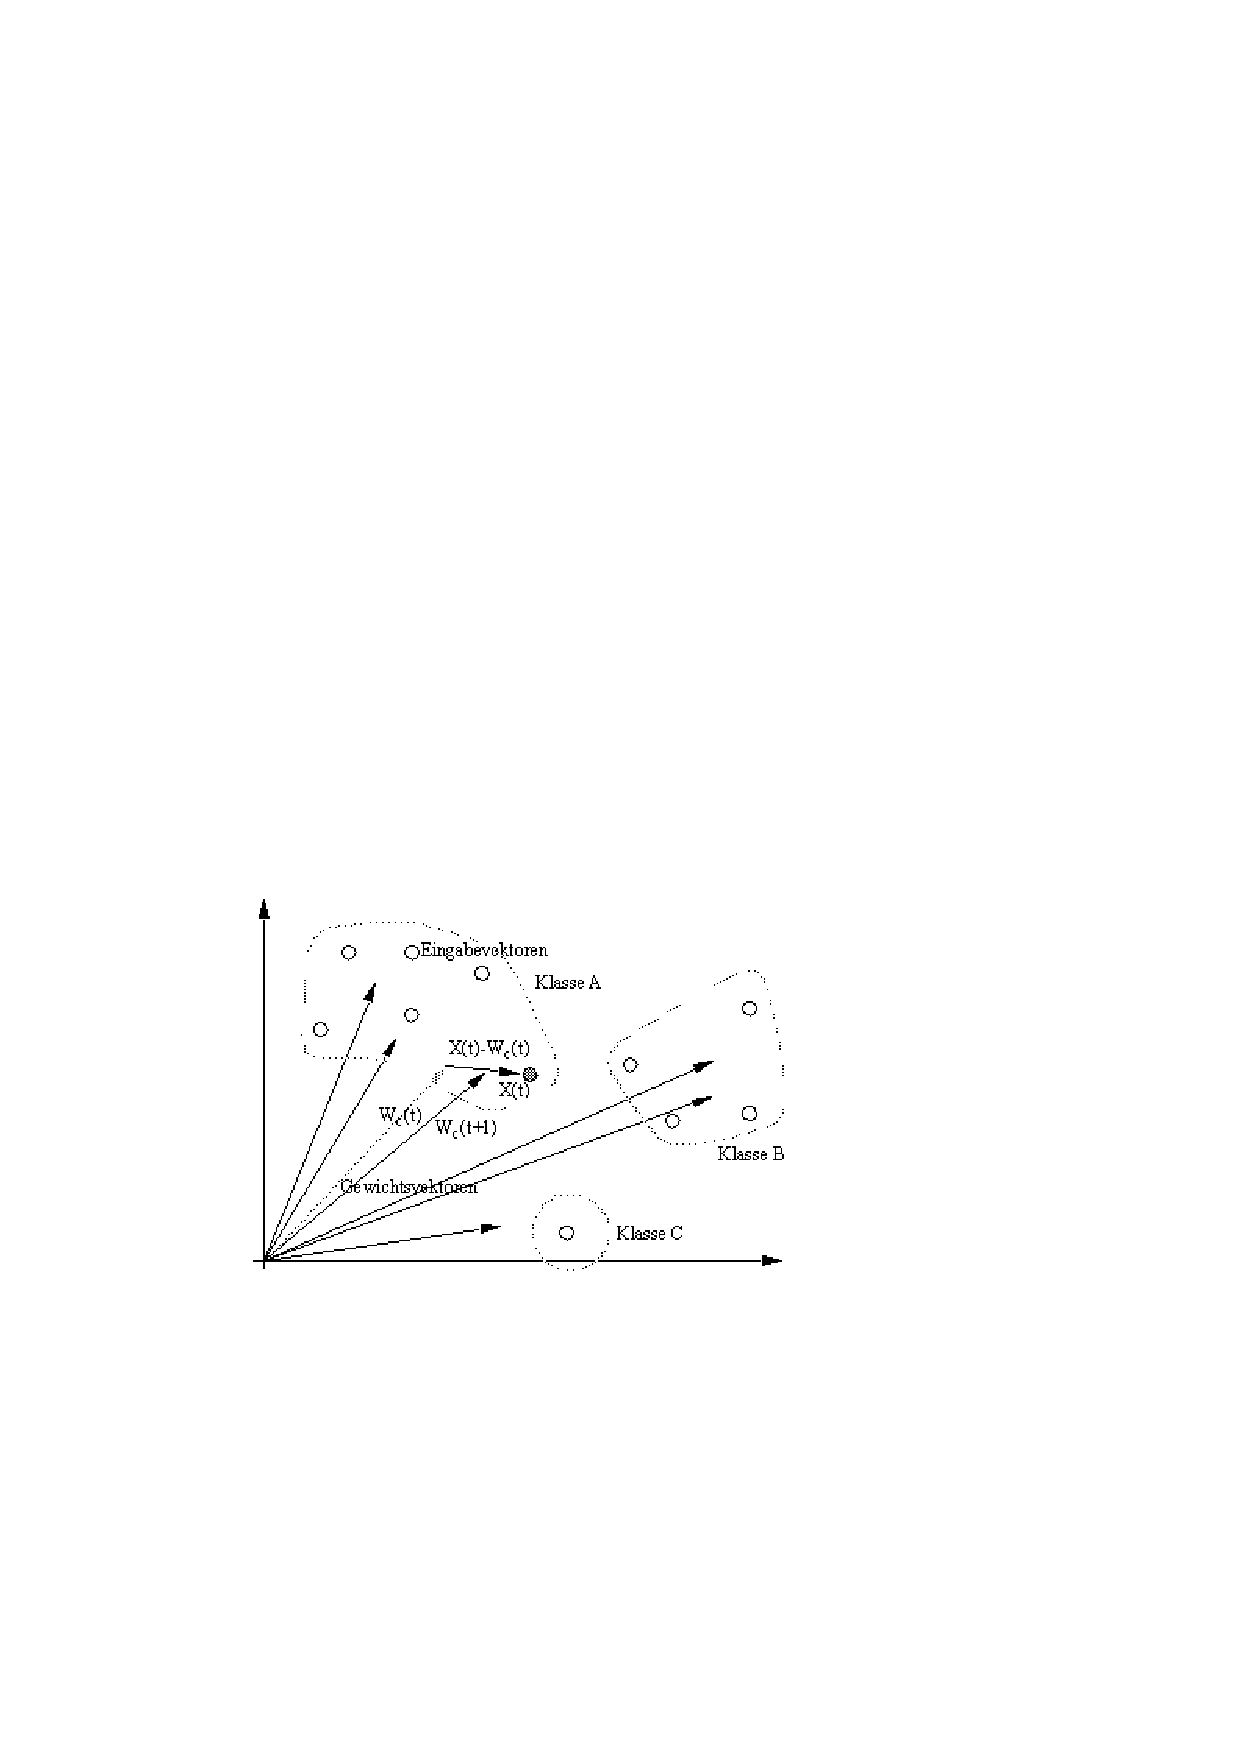
\includegraphics[width=\linewidth]{figures/ch07_lvq1.pdf}
	\caption{Adaption des nächsten Prototypvektors $W_c(t)$ zum Eingabevektor $X(t)$. Hier sind die Eingabevektoren als kleine Kreise, die Prototypvektoren als Pfeile dargestellt. Weiterhin ist hier $Klasse(X) = Klasse(W_c)$.}
	\label{fig:ch07_lvq1}
\end{figure}



% ----------------------------------------------------------------------
% ----------------------------------------------------------------------
\section*{LVQ2.1}
Bei dem Verfahren LVQ2.1 ist die Klassifikation der Eingabe identisch wie bei LVQ1, nur die Modifikation der Prototypvektoren beim Lernen ist anders.
LVQ2.1 sucht \emph{zwei} Prototypvektoren:
\begin{enumerate}
	\item Den \emph{nächsten} Prototypvektor $C_i$ und
	\item Den \emph{übernächsten} Prototypvektor $C_j$.
\end{enumerate}
Dabei findet nur dann eine Adaption der Prototypvektoren statt, wenn folgende Voraussetzungen erfüllt sind:
\begin{itemize}
	\item $Klasse(C_i) \ne Klasse(C_j)$
	\item $Klasse(p) = Klasse(C_i) \vee Klasse(p) = Klasse(C_j)$ 
	\item $p$ liegt in einem "`Fenster"' entlang der Mittelsenkrechten zwischen den beiden Klassen $Klasse(C_i)$ und $Klasse(C_j)$.
\end{itemize}

\subsection*{Das "`Fenster"'}
Wenn man mit $d_i$ und $d_j$ die euklidischen Abstände des Eingabevektors $p$ von den Vektoren $C_i$ und $C_j$ bezeichnet, dann fällt der Eingabevektor $p$ in ein Fenster mit relativer Breite $v$ falls gilt:
\[
	min(\frac{d_i}{d_j}, \frac{d_j}{d_i}) > s
	\quad \text{wobei } s = \frac{1-v}{1+v}
\]
Nach Kohonen sollte die Breite $v$ des relativen Fensters zwischen $0.2$ und $0.3$ betragen. Man beachte, dass dieses "`Fenster"' kein Rechteck ist.
Grafisch kann man sich das wie in Abbildung \ref{fig:ch07_lvq2} gezeigt veranschaulichen. Dort wurde der Wert $v=0.2$ verwendet, wodurch sich $s = \frac{2}{3}$ ergab.

\begin{figure}[ht!] \centering 
	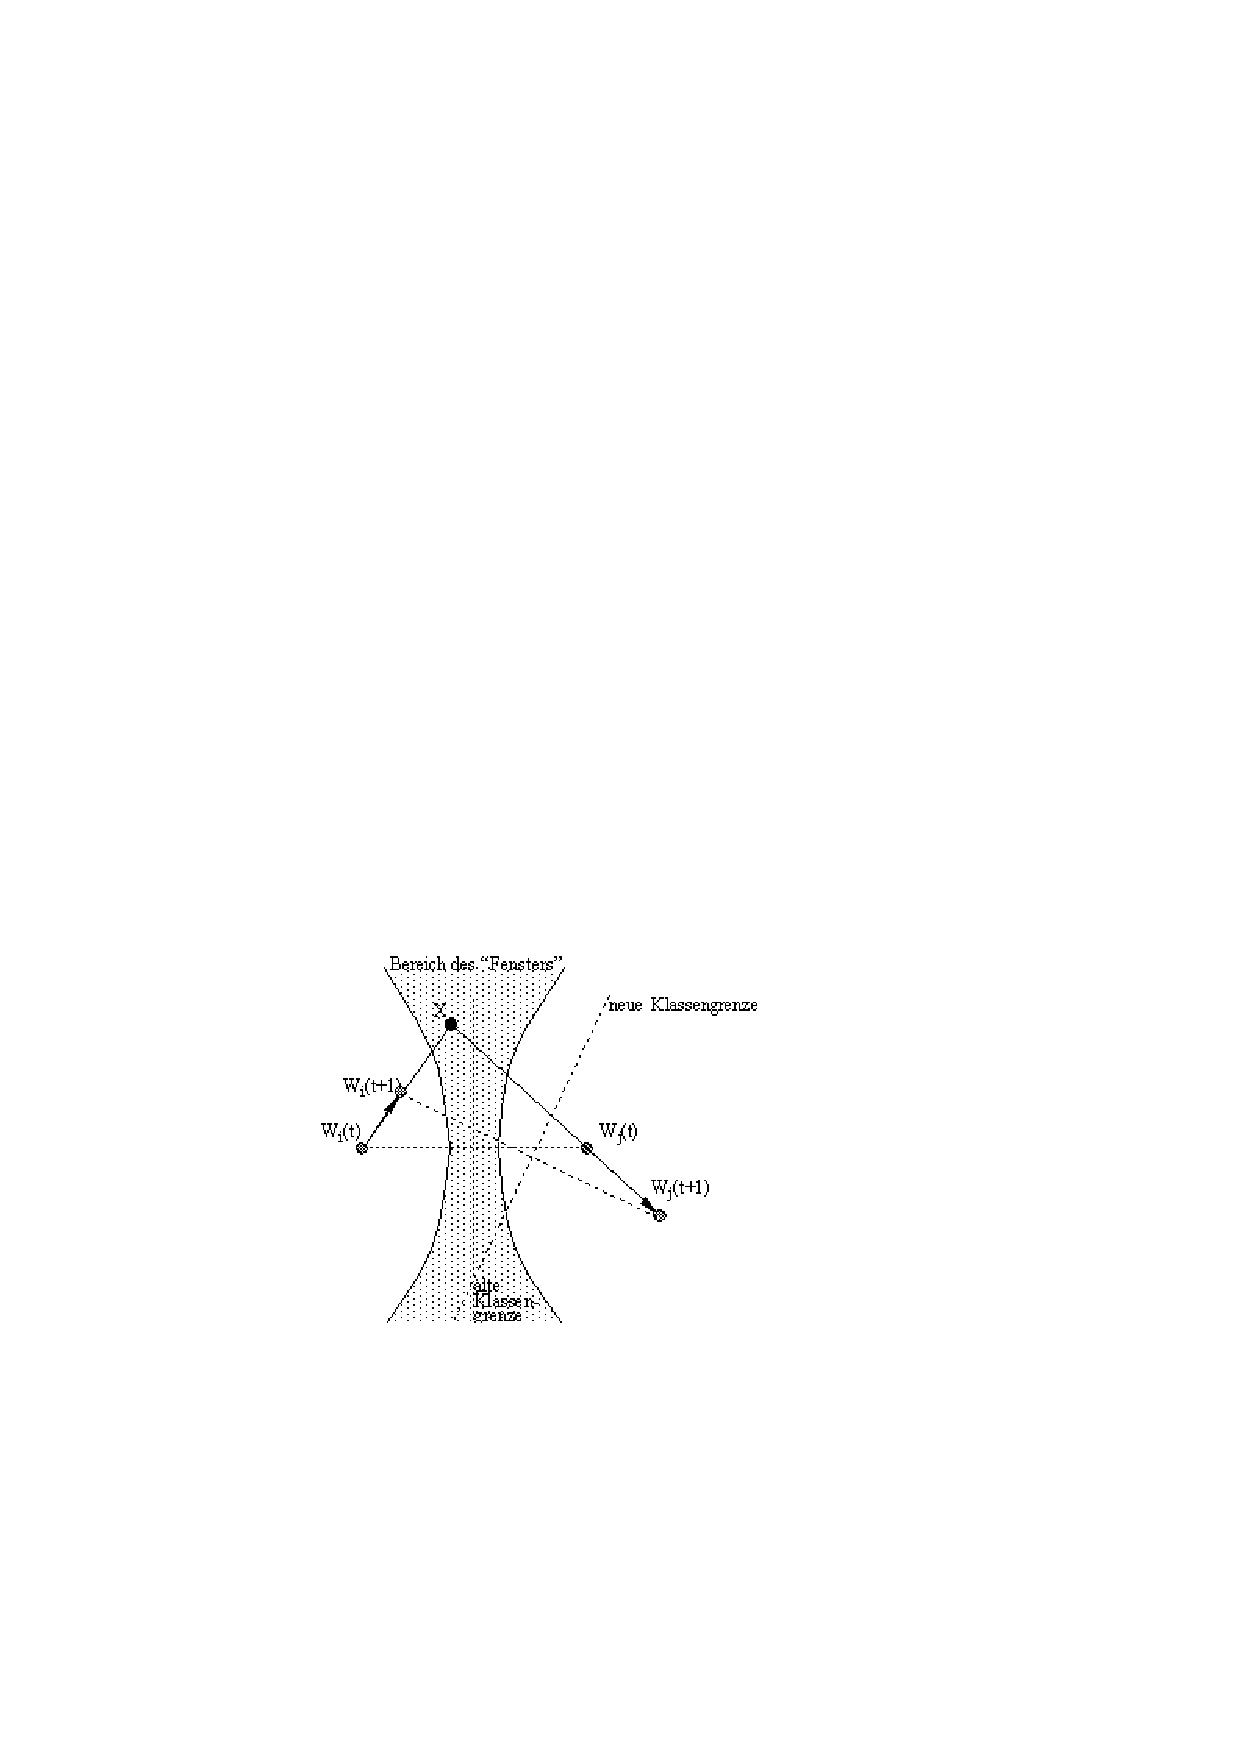
\includegraphics[width=\linewidth]{figures/ch07_lvq2.pdf}
	\caption{Prinzip von LVQ 2.1: Der Prototypvektor $W_i(t)$, dessen Klasse mit der des Musters $X$ übereinstimmt, wird in Richtung des Eingabevektors $X$ verschoben. Der nächste Vektor $W_j(t)$, dessen Klasse \emph{nicht} mit der des Musters $X$ übereinstimmt, wird von $X$ weggeschoben. Dadurch dreht sich die durch die Mittelsenkrechte der Verbindungslinien gebildete Klassengrenze.}
	\label{fig:ch07_lvq2}
\end{figure}
\noindent
Die Formeln für die Anpassung der Prototypvektoren lauten:
\begin{align*}
	C_i(t+1) &= C_i(t) + \eta(t) \Big( p(t) - C_i(t) \Big) \\
	C_j(t+1) &= C_j(t) - \eta(t) \Big( p(t) - C_j(t) \Big)
\end{align*}

Dieses Verfahren modifiziert nur die Grenzflächen der Klassen durch Verschieben der Vektoren, es garantiert jedoch nicht mehr, dass die Dichte
der Vektoren die Verteilungsdichte der Eingabevektoren annähert. Um diesen Mangel wieder zu beheben, wurde LVQ3 entwickelt.


% ----------------------------------------------------------------------
% ----------------------------------------------------------------------
\section*{LVQ3}
Das Verfahren LVQ3 ist eine Erweiterung des Verfahrens LVQ2.1, bei dem zusätzlich zur Änderung der Gewichtsvektoren an einer Klassengrenze die Vektoren $C_i$ und $C_j$ verändert werden, wenn beide der gleichen Klasse wie $X$ angehören.

Für die Anpassung der Prototypvektoren gilt (wie bei LVQ2.1):
\begin{align*}
	C_i(t+1) &= C_i(t) + \eta(t) \Big( p(t) - C_i(t) \Big) \\
	C_j(t+1) &= C_j(t) - \eta(t) \Big( p(t) - C_j(t) \Big)
\end{align*}
wenn die beiden nächsten Vektoren $C_i$ und $C_j$ verschiedenen Klassen angehören, $C_i$ zur gleichen Klasse gehört wie $p$, $C_j$ zu einer anderen Klasse, und $p$ in das "`Fenster"' an der Grenze der beiden Klassen fällt.

Wenn jedoch $C_i$ und $C_j$ der gleichen Klasse wie $p$ angehören, werden - im Gegensatz zu LVQ2.1 - auch beide geändert:
\begin{align*}
	C_i(t+1) &= C_i(t) + e \eta(t) \Big( p(t) - C_i(t) \Big) \\
	C_j(t+1) &= C_j(t) + e \eta(t) \Big( p(t) - C_j(t) \Big)
\end{align*}
Als gute Richtwerte von $e$ gelten Werte zwischen $0.1$ und $0.5$, wobei der Wert für $e$ von der Größe des Fensters abhängt und für engere Fenster besser kleiner zu wählen ist.


% ----------------------------------------------------------------------
% ----------------------------------------------------------------------
\section*{OLVQ1}
Für das Verfahren LVQ1 ist es möglich, die Lernrate für \emph{schnelle Konvergenz} des Verfahrens zu optimieren. Dies führt zum Verfahren OLVQ1. Das optimierte LVQ1 (optimized learning vector quantization, OLVQ1) ist eine Erweiterung von LVQ1, bei der jedem Prototypvektor (Codebookvektor) eine eigene Lernrate $\eta_c(t)$ zugewiesen wird:
\begin{align*}
	C_c(t+1) &= C_c(t) + h(t) \eta_c(t) \Big( p(t) - C_c(t) \Big)\\
	&\text{mit} \\
	\eta_c(t) &= \frac{\eta_c(t-1)}{1 + h(t) \eta_c(t-1)}
\end{align*}
\noindent
Wobei für $h(t)$ gilt:
\[
	h(t) = 
	\begin{cases}
		+1 &\text{wenn } Klasse(C_c) = Klasse(p) \\
		-1 &\text{wenn } Klasse(C_c) \ne Klasse(p)
	\end{cases}
\]

Dies ist die Regel für die optimale Änderung der Lernfaktoren $\eta_c(t)$. Da $\eta_c(t)$ auch anwachsen kann, aber nicht über den Wert $1$ wachsen
darf (andernfalls wird der Vektor nicht zu $p$ hingezogen, sondern über die Verbindungslinie hinter $p$ hinaus bewegt), muss sichergestellt werden, dass $\eta_c(t)$ nicht über $1$ anwächst. 



% ----------------------------------------------------------------------
% ----------------------------------------------------------------------
\section*{Unterschiede}
LVQ3 ist stabiler als LVQ2.1, ein fortlaufendes Lernen verändert optimal eingestellte Gewichtsvektoren nicht mehr.
Die beiden Verfahren LVQ1 und LVQ3 passen die Lage der Codebookvektoren der Verteilung der Eingabevektoren an, während LVQ2.1 nur die relativen Entfernungen der Codebookvektoren von der Grenzlinie zwischen den Klassen optimiert. Dies garantiert nicht, dass diese Vektoren optimal platziert sind, um die Form der Klassengrenze anzunähern. LVQ2.1 sollte daher in erster Linie zur schärferen Klassentrennung mit einer kleinen Lernrate und einer relativ kleinen Zahl von Lernschritten verwendet werden.


% ----------------------------------------------------------------------
% ----------------------------------------------------------------------
\section*{Bemerkungen}
Die Genauigkeit, mit der eine Klassifikationsaufgabe mit LVQ gelöst werden kann, hängt von einer Reihe von Faktoren ab:

\begin{itemize}
	\item der Zahl der verfügbaren Codebookvektoren für jede Klasse
	\item der Initialisierung der Codebookvektoren
	\item dem verwendeten Lernalgorithmus
	\item der richtigen Lernrate für die einzelnen Schritte
	\item einem richtigen Abbruchkriterium zur Terminierung des Lernens
\end{itemize}

\subsection*{Codebookvektoren}
Für viele Anwendungen ist es ausreichend, mit einer gleichen Anzahl von Codebookvektoren (Neuronen) für jede Klasse zu arbeiten, selbst wenn die a-priori-Wahrscheinlichkeiten der Zugehörigkeit der Eingabemuster zu den einzelnen Klassen stark differieren.
Eine obere Grenze für die Gesamtzahl der Codebookvektoren ist zumeist die begrenzte Rechenzeit beim Training oder bei der Klassifikation in der Arbeitsphase.

Für die Anfangsinitialisierung der Codebookvektoren wählt man oft als
Initialwerte Vektoren aus den Trainingsdaten aus. Damit verhindert man, dass Codebookvektoren Initialwerte besitzen, die weit entfernt von den Werten der Trainingsmuster sind. Diese Vektoren wären dann nämlich nie die nächsten Nachbarn zu den Eingabevektoren und würden nie verändert werden.

\subsection*{Training}
Die Grenzen der Erkennungsgenauigkeit werden nach einer Zahl von Lernschritten erreicht, die der 30- bis 50-fachen Zahl der Codebookvektoren entspricht, d.h. jedes Neuron wird im Mittel zwischen 30 und 50 Mal verändert.

Läßt man die LVQ-Verfahren zu lange lernen, so tritt oft der Effekt des \emph{Übertrainierens} auf.
Der Trainingsvorgang sollte daher nicht unbegrenzt fortgeführt werden, sondern nach einer Schrittzahl, die ca. der 50- bis 200-fachen Zahl der Codebookvektoren entspricht (abhängig von Algorithmus und Lernrate), abgebrochen werden. Die Schrittzahl ist natürlich auch abhängig von den Eingabevektoren und damit vom Problem.



\section{Selbstorganisierende Karten (SOM)}
% 15
\begin{hint}{Achtung!}{unvollstaendig-som}
	Dieser Abschnitt der Zusammenfassung ist sehr wahrscheinlich unvollständig und sollte überarbeitet werden!
	Aus Zeitgründen wurden hier nicht alle Themen der Vorlesung erarbeitet.
	\begin{flushright}\textit{Beni}\end{flushright}
\end{hint}
\noindent
Die selbstorganiserenden Karten (engl. self-organizing maps (SOM), auch Kohonen Maps oder Kohonen Feature Maps) sind eng verwand mit der lernenden Vektorquantisierung (LVQ). Man kann sie als Weiterentwicklung von LVQ unter Betrachtung einer \emph{lokalen Nachbarschaftsbeziehung} der Neuronen betrachten.


% ------------------------------------------------------------------------
% ------------------------------------------------------------------------
\section*{Prinzip}
Bei den selbstorganisierenden Karten handelt es sich wieder um einschichtige neuronale Netze mit einer Schicht aktiver Neuronen. Die selbstorganisierenden Karten werden im Gegensatz zu LVQ aber mit \emph{unüberwachten} Lernverfahren trainiert.

Die Ausgabe der SOMs ist deren Zustand: Es ist nicht interessant, was die Neuronen berechnen und ausgeben, sondern nur welches Neuron gerade aktiv ist. Damit sind SOMs wesentlich biologieverwandter als beispielsweise feedforward-Netze.



% ------------------------------------------------------------------------
% ------------------------------------------------------------------------
\section*{Aufbau}
SOMs haben - wie das Gehirn - typischerweise die Aufgabe, einen hochdimensionalen Input ($N$ Dimensionen) auf Bereiche in einem niedrigdimensionalen Gitter ($G$ Dimensionen) abzubilden, also sozusagen eine \emph{Karte} von dem hochdimensionalen Raum zu zeichnen. Um diese Karte zu erschaffen, erhält die SOM einfach beliebig viele Punkte aus dem Inputraum.
Die SOM wird während der Eingabe der Punkte versuchen, die Orte, auf denen die Punkte auftreten, so gut wie möglich mit ihren Neuronen abzudecken. Dies bedeutet insbesondere, dass jedes Neuron einem bestimmten Ort im Inputraum zuzuordnen ist.

Es gibt damit zwei Räume, in denen SOMs arbeiten:
\begin{itemize}
	\item \emph{N-dimensionaler Eingaberaum}
	\item \emph{G-dimensionales Gitter} - Stellt die Nachbarschaftsbeziehungen der Neuronen und damit die Netztopologie dar. 
\end{itemize}

Wichtig: Auch dann, wenn $N = G$ gilt, sind die beiden Räume nicht gleich und müssen unterschieden werden. Sie haben in diesem Spezialfall nur die gleiche Dimension.

\subsection*{Gitterstruktur}
Folgende Gitterstrukturen sind üblich:
\begin{itemize}
	\item \emph{eindimensionale} Gitter - Anordnung wie bei einer Perlenkette (siehe Abbildung ? oben). Jedes Neuron besitzt genau zwei Nachbarn (außer die beiden Endneuronen).
	\item \emph{zweidimensionale} Gitter - Rechtwinklige (siehe Abbildung ? unten) oder wabenförmige Anordnungen. Auch ungleichmäßige Topologien sind möglich, jedoch nicht sehr häufig.
	\item \emph{mehrdimensionale} Gitter - Topologien mit mehr Dimensionen und wesentlich mehr Nachbarschaftsbeziehungen wären auch denkbar, werden aber aufgrund der mangelnden Visualisierungsfähigkeit nicht oft eingesetzt.
\end{itemize}

\begin{figure}[ht!] \centering 
	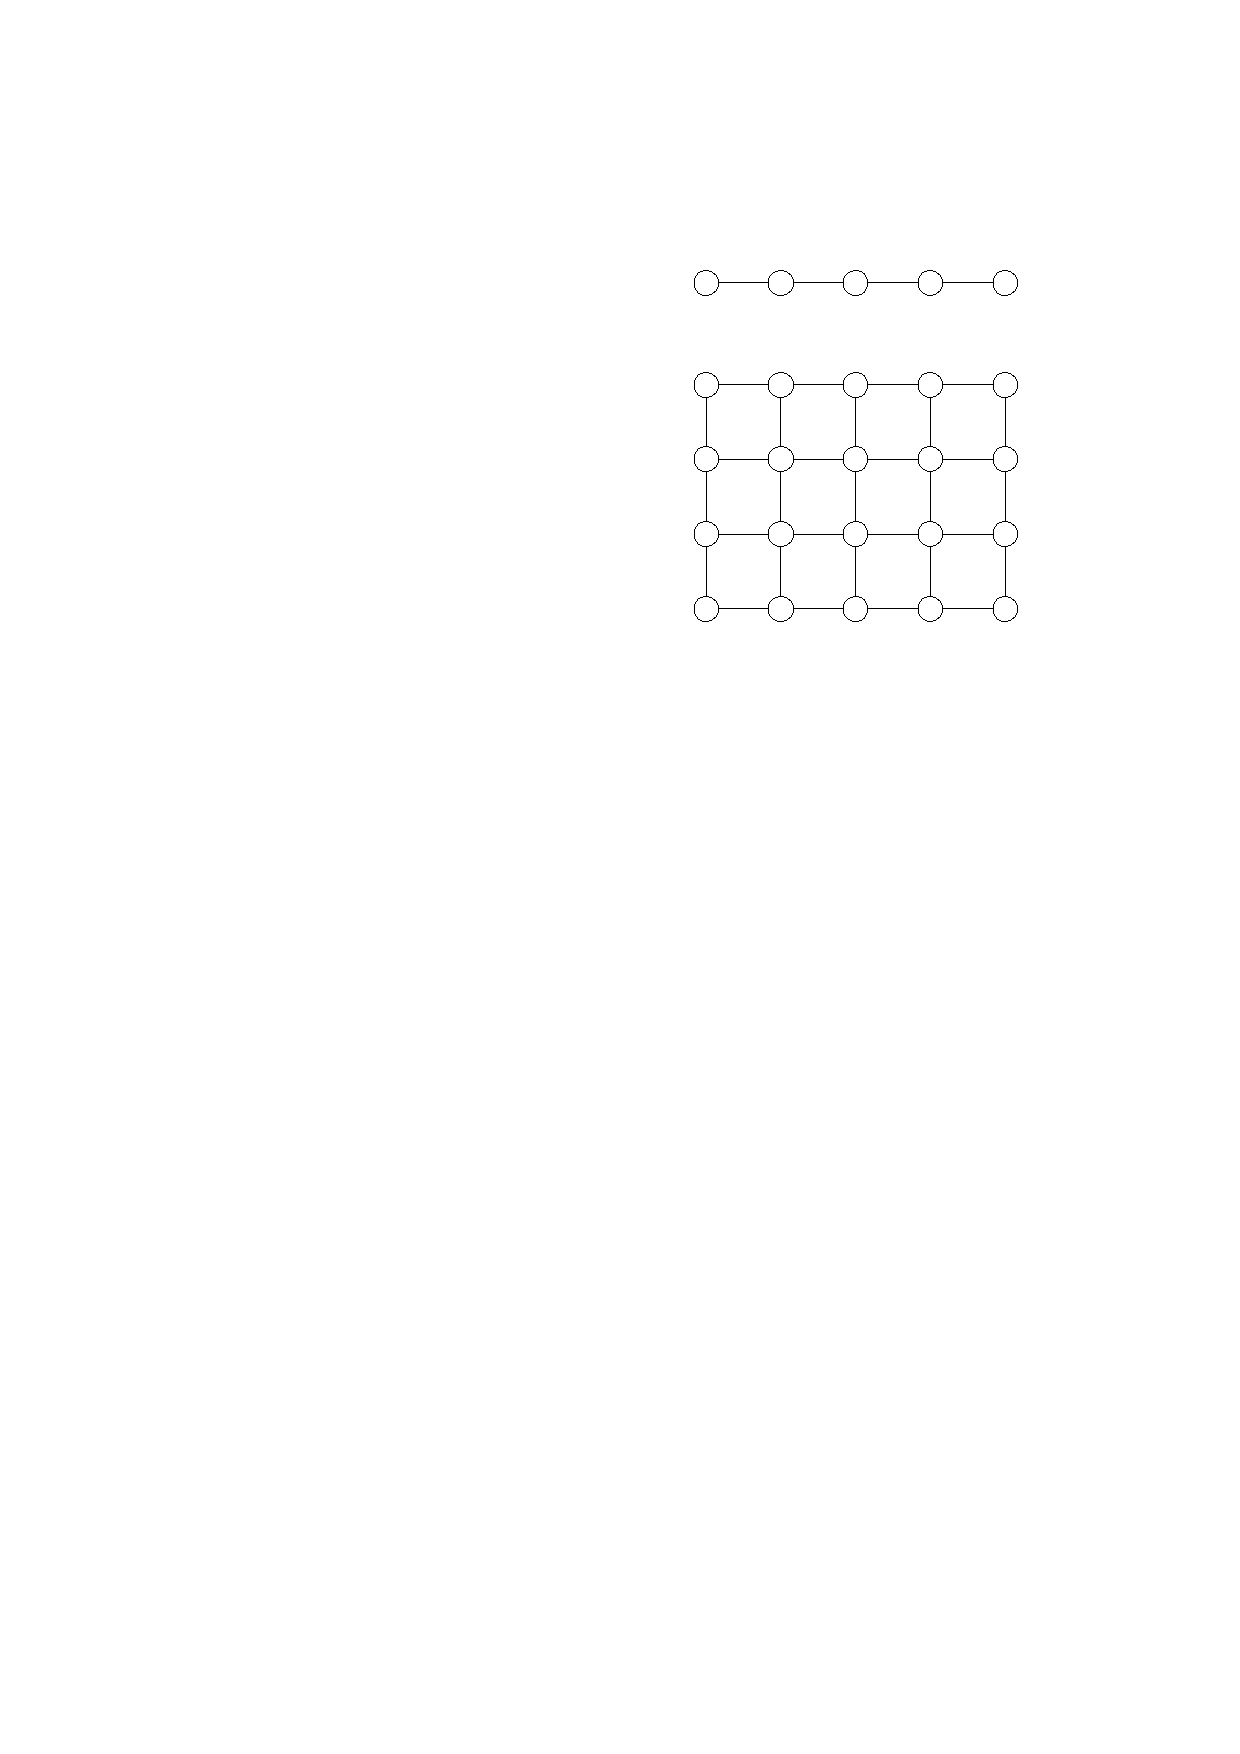
\includegraphics[width=0.5\linewidth]{figures/ch08_som-gitter.pdf}
	\caption{Beispieltopologien einer Self Organizing Map - Oben eine eindimensionale Topologie, unten eine zweidimensionale.}
	\label{fig:ch08_som-gitter}
\end{figure}


\subsection*{SOM-Neuron}
Ein SOM-Neuron $k$ besitzt eine feste Position $c_k$ (\emph{Zentrum} genannt) im Eingaberaum.


\subsection*{SOM}
Eine Self Organizing Map ist eine Menge $K$ von SOM-Neuronen. Bei Eingabe eines Eingabevektors wird genau dasjenige Neuron $k \in K$ aktiv, welches dem Eingabemuster im Eingaberaum am nächsten liegt.


\subsection*{Topologie}
Die Neuronen sind untereinander durch Nachbarschaftsbeziehungen verbunden. Diese Beziehungen nennt man \emph{Topologie}. Sie nimmt starken Einfluss auf das Training einer SOM und wird durch die Topologiefunktion $h(i,k,t)$ definiert.
Dabei ist $i$ das Gewinnerneuron, $k$ das gerade zu adaptierende Neuron und $t$ der Zeitschritt.


% ------------------------------------------------------------------------
% ------------------------------------------------------------------------
\section*{Funktionsweise}
Die Funktionsweise eine SOM teilt sich in die folgenden Schritte auf:

\begin{itemize}
	\item \emph{Eingabe} - Beliebiger Wert $p$ aus dem Eingaberaum $\mathbb{R}^N$.
	\item \emph{Abstandsberechnung} - Es wird der Abstand von jedem SOM-Neuron $k$ zur Eingabe $p$ berechnet: $||p - c_k||$
	\item \emph{Aktivierung} - \emph{Ein} Neuron wird aktiv, nämlich genau das Neuron $i$ mit dem kürzesten zuvor berechneten Abstand zur Eingabe $p$. Alle anderen Neuronen sind inaktiv (\emph{Winner-Takes-All-Schema}).
	\item \emph{Ausgabe} - Die Ausgabe der SOM ist \emph{welches} Neuron aktiv ist. 
\end{itemize}


% ------------------------------------------------------------------------
% ------------------------------------------------------------------------
\section*{Training}
Die Frage des Trainings ist, welches SOM-Neuron $k$ bei welcher Eingabe $p$ aktiv wird.

Das Training einer SOM unterteilt sich in fünf (zum Teil der Funktionsweise recht ähnliche) Schritte:

\begin{enumerate}
	\item \emph{Initialisierung} - Start des Netzes mit zufälligen Neuronenzentren $c_k \in \mathbb{R}^N$ aus dem Eingaberaum.
	\item \emph{Anlegen eines Eingabemusters} - Es wird ein Punkt $p$ aus dem Eingaberaum $\mathbb{R}^N$ (auch \emph{Stimulus} genannt) gewählt und in das Netz eingegeben.
	\item \emph{Abstandsmessung} - Für jedes SOM-Neuron $k$ im Netz wird nun der Abstand $||p - c_k||$ bestimmt.
	\item \emph{Winner takes all} - Es wird das \emph{Gewinnerneuron} $i$ ermittelt, welches den kleinsten Abstand zu $p$ besitzt, das also der Bedingung
	\begin{align*}
		||p - c_i|| \le ||p - c_k|| \quad \forall k \ne i
	\end{align*}
	\noindent
	genügt.\footnote{Bei mehreren Gewinnerneuronen kann eines nach Belieben gewählt werden.}
	\item \emph{Adaption der Zentren} - Die Zentren $c_k$ der SOM-Neurone werden innerhalb des Eingaberaums nach der Vorschrift
	\begin{align*}
		\Delta c_k = \eta(t) \cdot h(i,k,t) \cdot (p-c_k)
	\end{align*}
	\noindent
	versetzt, wobei die Werte $\Delta c_k$ einfach auf die bisherigen Zentren addiert werden:
	\begin{align*}
		c_k(t+1) = c_k(t) + \Delta c_k(t)
	\end{align*}
	\noindent
	Damit ist die Ortsänderung der SOM-Neuronen $k$ proportional zu der Entfernung zum eingegebenen Muster $p$, sowie zur zeitabhängigen Lernrate $\eta(t)$.\\
	Die \emph{Topologie} nimmt ihren Einfluss durch die Topologiefunktion $h(t,k,t)$, welche im Folgenden näher erläutert wird.
\end{enumerate}

\begin{figure}[ht!] \centering 
	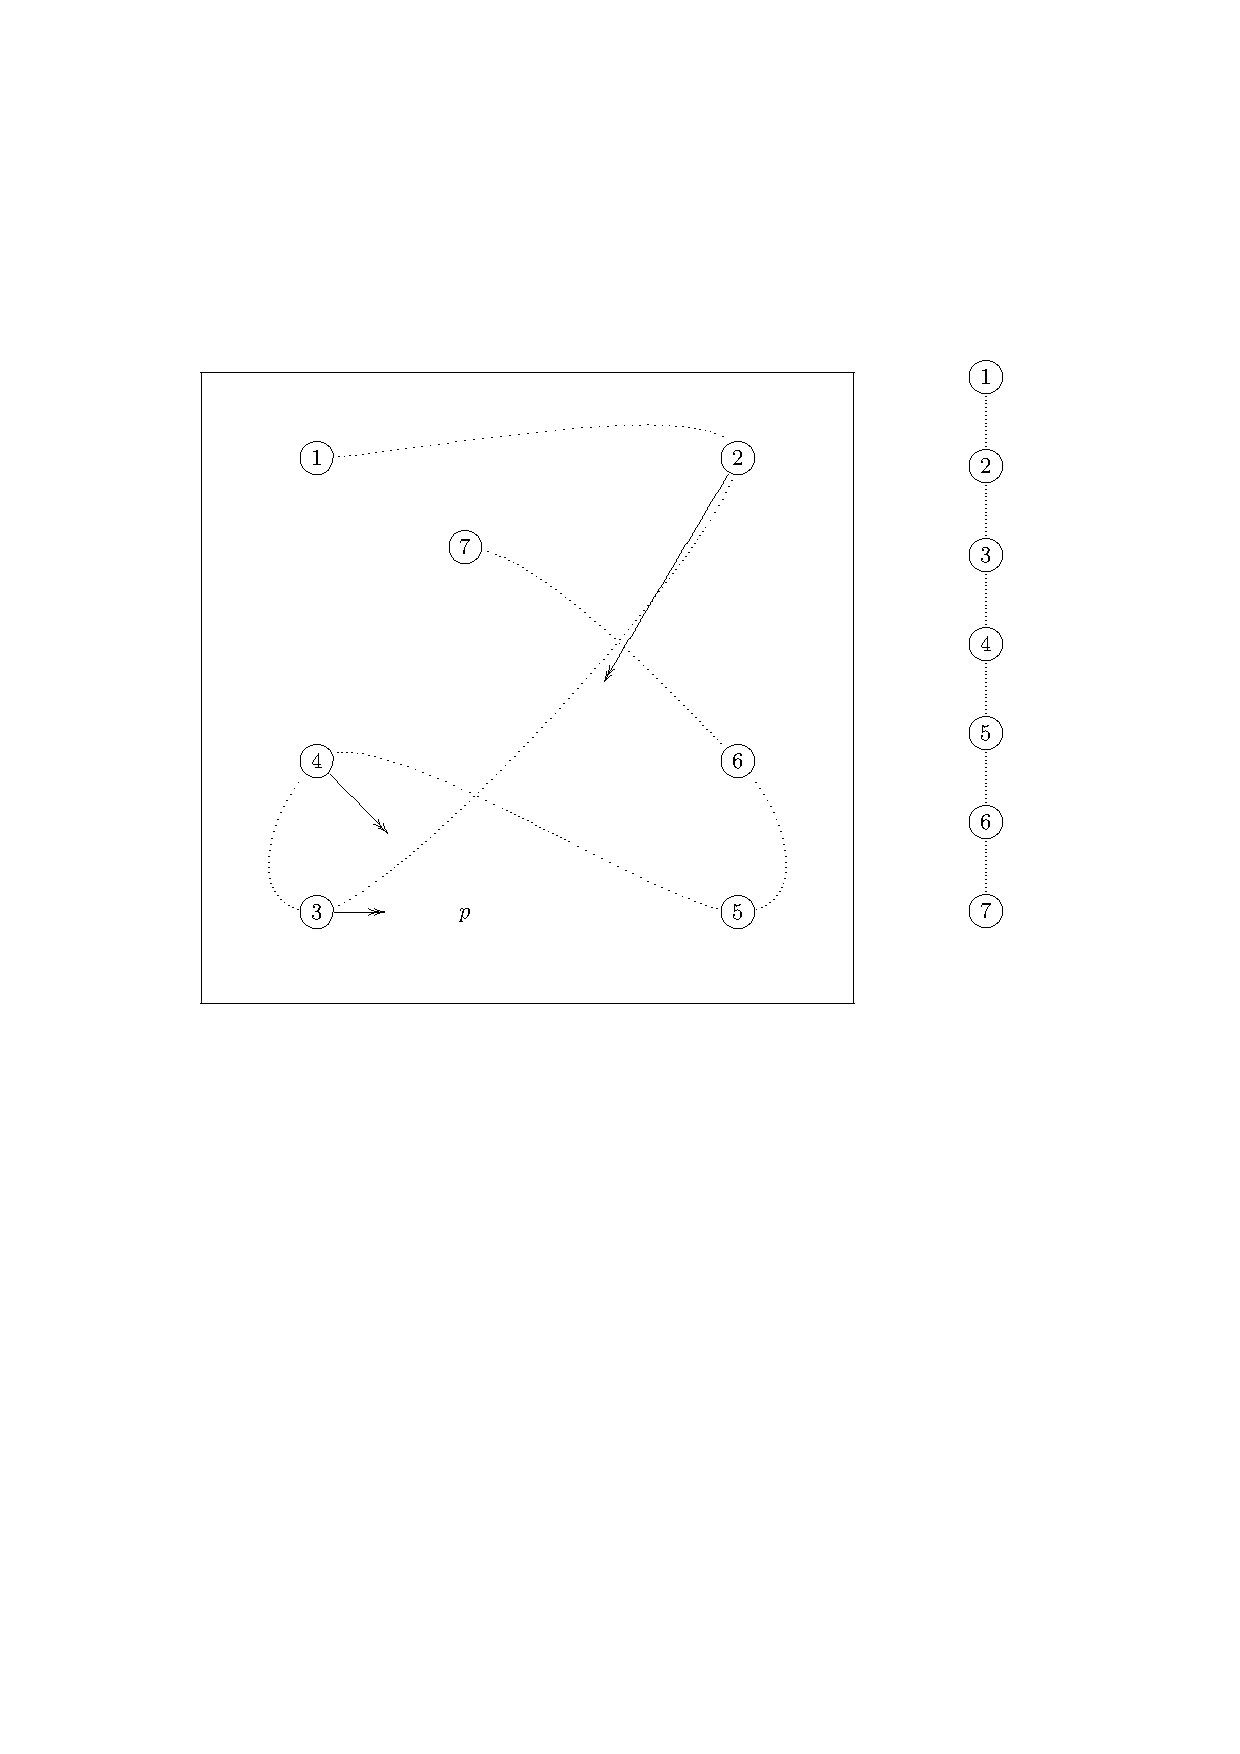
\includegraphics[width=\linewidth]{figures/ch08_som-training.pdf}
	\caption{Darstellung des zweidimensionalen Eingaberaumes (links) und des eindimensionalen Topologieraumes (rechts) einer SOM. Neuron 3 ist das Gewinnerneuron, da es $p$ am nächsten liegt. Die Nachbarn von Neuron 3 in der \emph{Topologie} sind die Neurone 2 und 4. Die Pfeile markieren die Bewegung des Gewinnerneurons und seiner Nachbarn in Richtung des Trainingsbeispiels $p$.}
	\label{fig:ch08_som-training}
\end{figure}

In Abbildung \ref{fig:ch08_som-training} wird ein beispielhafter Trainingsschritt abgebildet. Die eindimensionale Topologie der SOM ist zur Veranschaulichung durch die gepunkteten Linien in den Eingangsraum aufgetragen.

Obwohl das Zentrum von Neuron 7 vom \emph{Eingangsraum} aus gesehen wesentlich näher am Eingangsmuster $p$ liegt als das Neuron 2, lernt das Neuron 2, und das Neuron 7 nicht.
An dieser Stelle sei darauf hingewiesen, dass die \emph{Netztopologie} bestimmt, welches Neuron lernen darf und nicht die Lage im Eingangsraum.
Dies ist genau der Mechanismus, durch den eine Topologie einen Eingangsraum aussagekräftig abdecken kann, ohne mit ihm auf irgendeine Weise verwandt sein zu müssen.


\subsection*{Topologiefunktion}
Die Topologiefunktion $h(i,k,t)$ bestimmt, wie stark ein lernendes Neuron seine Nachbarn beeinflusst. Sie ist nicht auf dem Eingaberaum, sondern auf dem Gitter definiert und stellt die Nachbarschaftsbeziehung der SOM-Neuronen dar.

Prinzipiell ist der Sinn der Funktion, einen großen Wert anzunehmen, falls $k$ Nachbar des Gewinners oder gar der Gewinner selbst ist, und kleine Werte, falls nicht.
Schärfer definiert: Die Topologiefunktion muss \emph{unimodal} sein, also genau ein Maximum besitzen - dieses Maximum muss beim Gewinnerneuron $i$ liegen, das zu sich selbst natürlich die Entfernung $0$ hat.

Um große Werte für Nachbarn von $i$ und kleine Werte für Nicht-Nachbarn ausgeben zu können, braucht die Funktion $h$ eine Art \emph{Abstandsbegriff} auf dem Gitter. Dafür gibt es verschiedene Methoden (siehe Abbildung ).

\begin{figure}[ht!] \centering 
	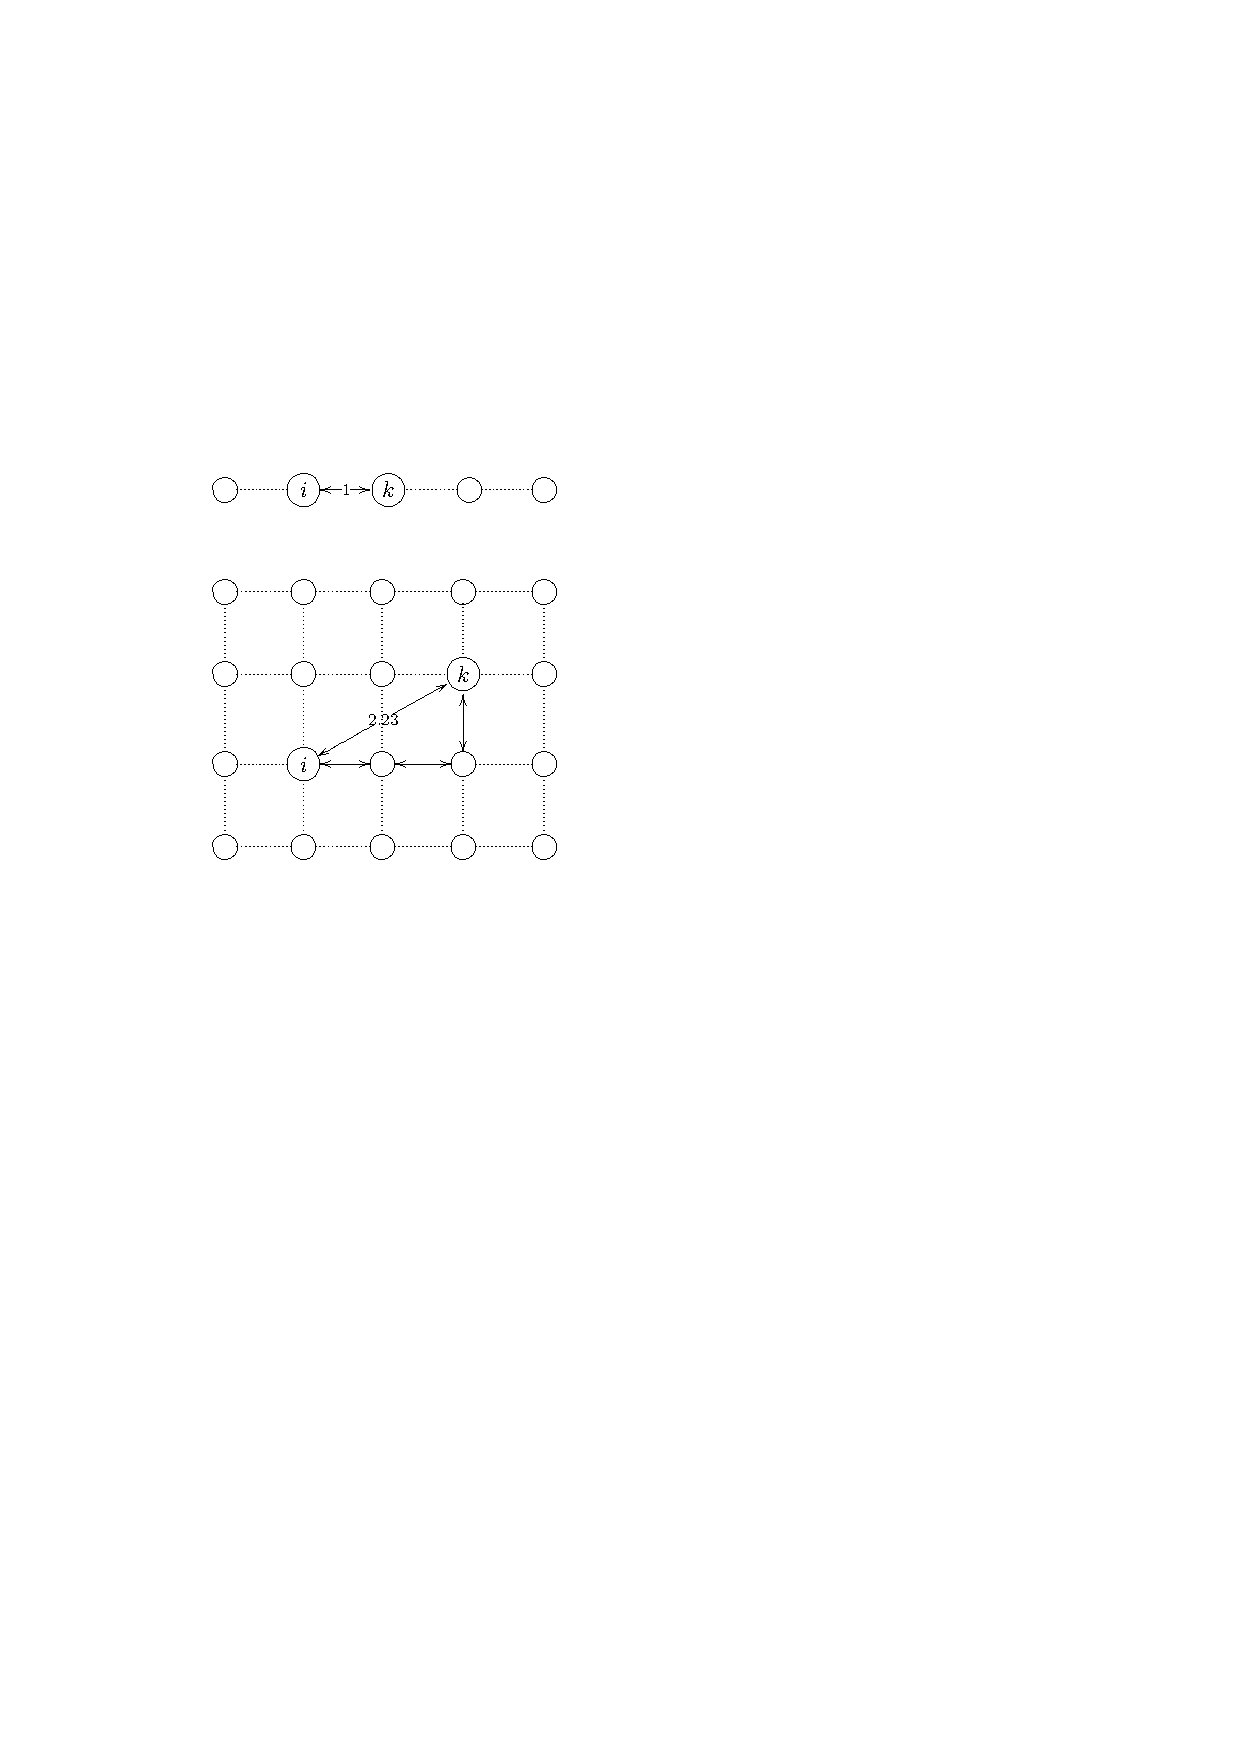
\includegraphics[width=0.5\linewidth]{figures/ch08_som-abstand-auf-gitter.pdf}
	\caption{Beispielabstände einer eindimensionalen (oben) und einer zweidimensionalen SOM-Topologie (unten) zwischen zwei SOM-Neuronen $i$ und $k$.}
	\label{fig:ch08_som-abstand-auf-gitter}
\end{figure}

Bei eindimensionalen Gittern kann die Anzahl der Verbindungen (diskrete Weglänge) zwischen $i$ und $k$ abgezählt werden.
Bei zweidimensionalen Gittern wird der Euklidische Abstand für die Abstandsberechnung herangezogen.

Eine \emph{Zeitabhängigkeit} ist optional, wird aber oft verwendet, um die Nachbarschaft mit der Zeit schrumpfen zu lassen.
Der Vorteil bei einer sinkenden Nachbarschaftsgröße ist, dass ein sich bewegendes Neuron zu Anfang viele Neurone in seiner Umgebung "`mitzieht"', sich das zufällig initialisierte Netz also am Anfang schnell und sauber entfalten kann.
Zum Ende des Lernvorganges hin werden nur noch wenige Neurone auf einmal beeinflusst, was das Netz im Gesamten steifer macht, aber ein gutes "`fine tuning"' der einzelnen Neurone ermöglicht.

\begin{figure}[ht!] \centering 
	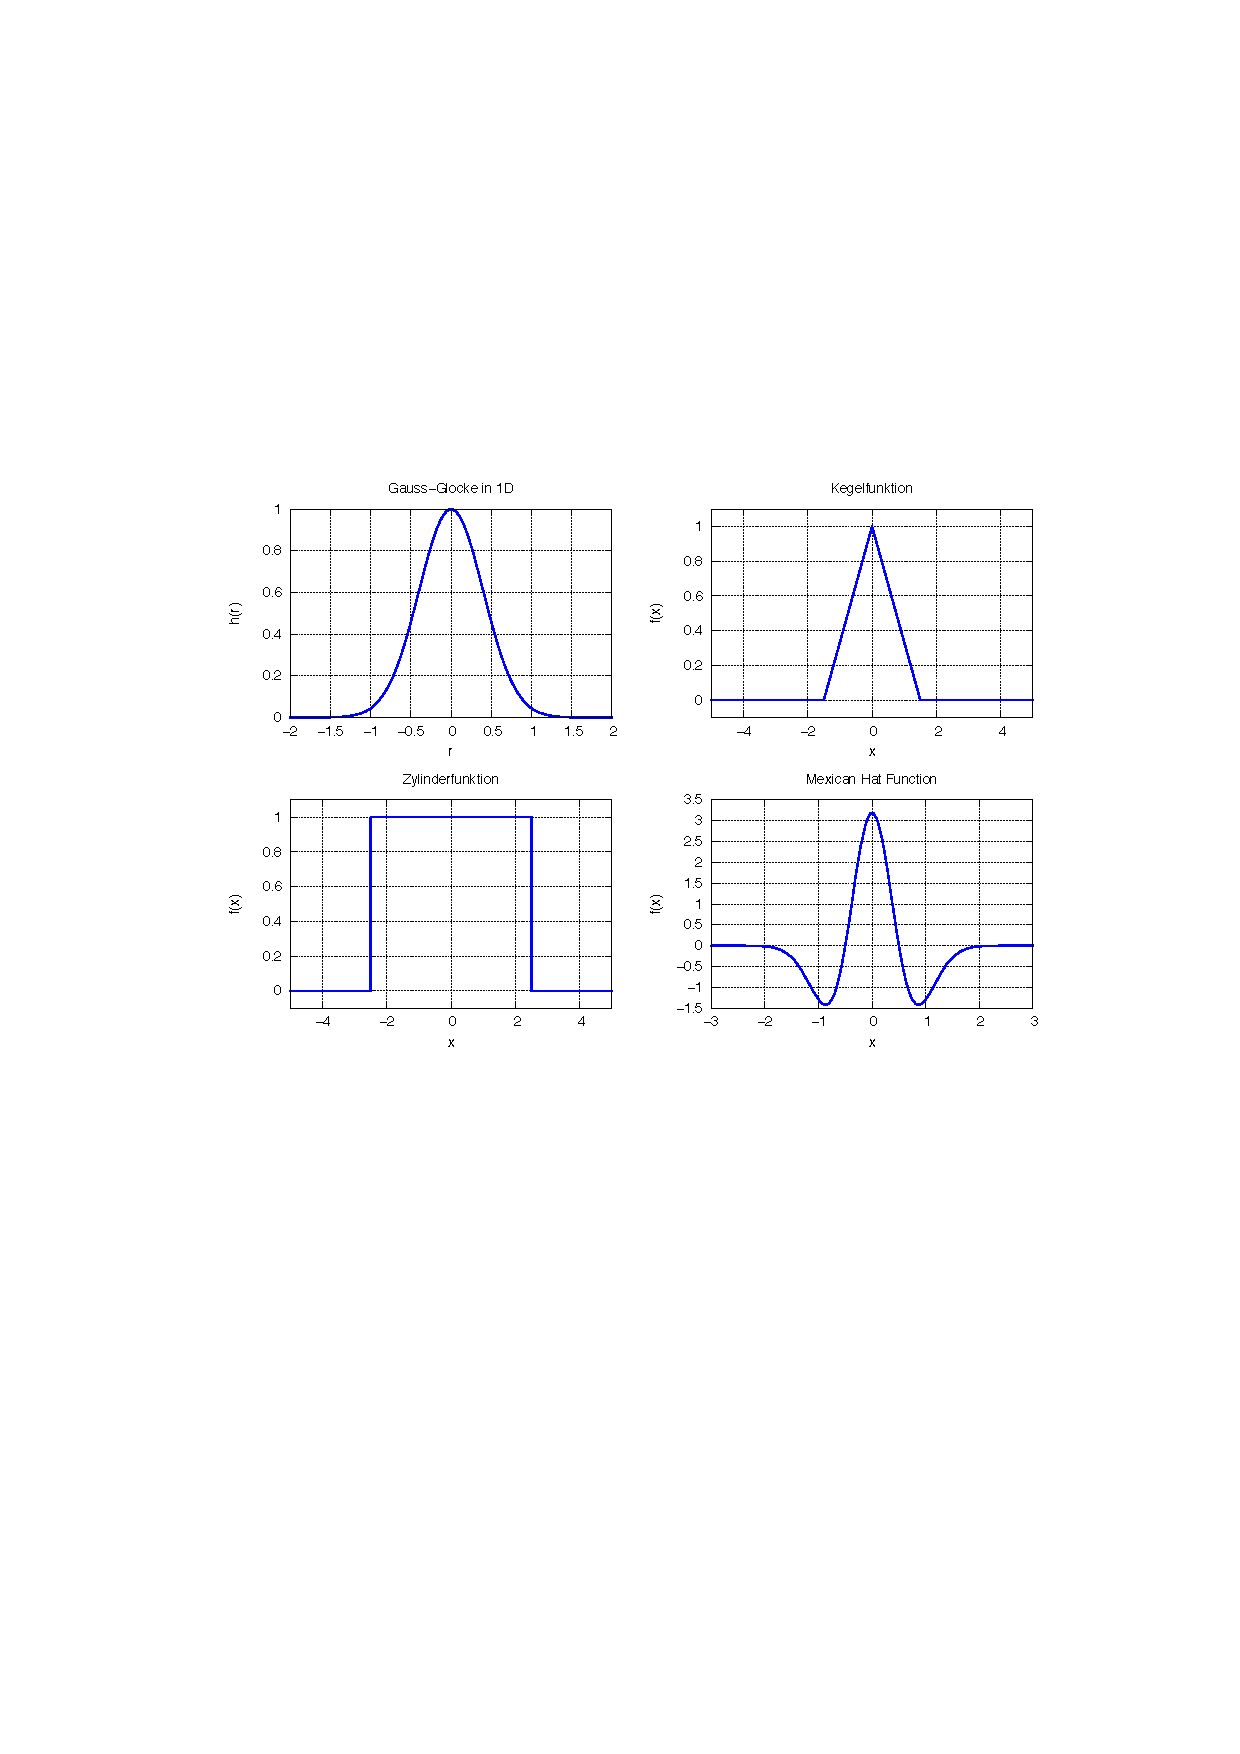
\includegraphics[width=\linewidth]{figures/ch08_som-topologiefunktionen.pdf}
	\caption{Mögliche Topologiefunktionen einer SOM: Gaußglocke, Kegelfunktion, Zylinderfunktion und die von Kohonen vorgeschlagene Mexican-Hat-Funktion.}
	\label{fig:ch08_som-topologiefunktionen}
\end{figure}


\subsubsection*{Gaußglocke}
Eine gängige Abstandsfunktion ist die \emph{Gaußglocke}. Sie ist unimodal mit einem Maximum bei 0 und kann zusätzlich durch den Parameter $\sigma$ in ihrer Breite verändert werden. Dies kann für die Realisierung der über die Zeit schrumpfenden Nachbarschaft genutzt werden.

Die Topologiefunktion hat dann die Form
\[
	h(i,k,t) = e^{\big(- \frac{||g_i - g_k||^2}{2 \cdot \sigma(t)^2}\big)}
\]
wobei $g_i$ und $g_k$ die Positionen der SOM-Neurone $i$ und $k$ \emph{auf dem Gitter}\footnote{Die Positionen im \emph{Eingaberaum} werden mit $c_i$ und $c_k$ bezeichnet.} bezeichnen.

\subsubsection*{Andere Topologiefunktionen}
Weitere Funktionen, die anstatt der Gaußfunktion eingesetzt werden können, sind zum Beispiel die Kegelfunktion, die Zylinderfunktion oder die Mexican-Hat-Funktion (siehe Abbildung \ref{fig:ch08_som-topologiefunktionen}).
Die Mexican-Hat-Funktion bietet hierbei eine besondere biologische Motivation: Sie stößt durch ihre negativen Stellen manche Neurone in der Umgebung des Gewinnerneurons ab, was man auch in der Natur schon beobachtet hat.
Dies kann für schärfere Abgrenzung der Kartenbereiche sorgen - genau aus diesem Grund wurde sie auch von Teuvo Kohonen selbst vorgeschlagen.


\subsection*{Entwicklung einer SOM}
Abbildung \ref{fig:ch08_som-entwicklung} zeigt wie sich eine eindimensionale SOM im zweidimensionalen Eingaberaum bei gleichverteilten Eingabemustern über die Zeit entwickeln kann.

\begin{figure}[ht!] \centering 
	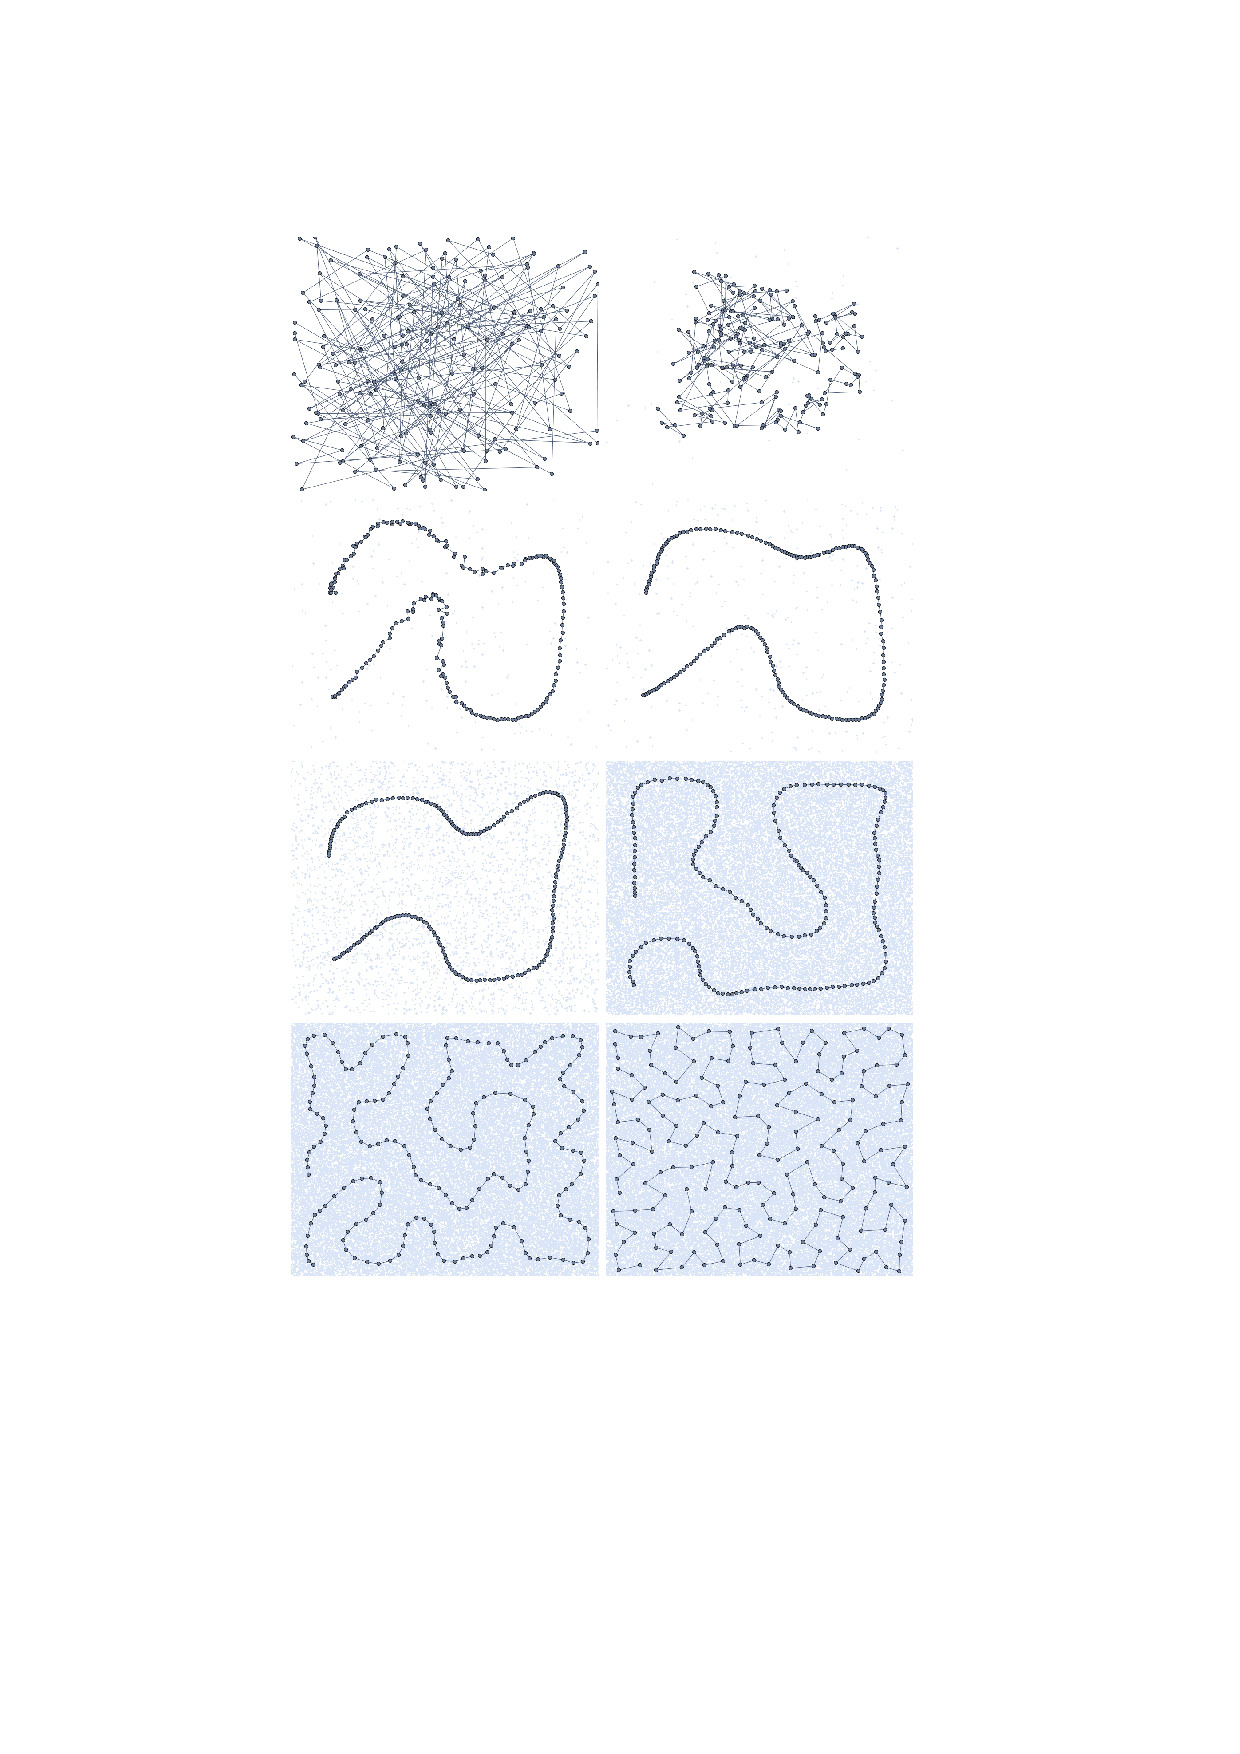
\includegraphics[width=\linewidth]{figures/ch08_som-entwicklung.pdf}
	\caption{Verhalten einer SOM mit eindimensionaler Topologie $(G = 1)$ nach Eingabe von 0, 100, 300, 500, 5000, 50000, 70000 und 80000 zufällig verteilten Eingabemustern $p \in R^2$. $\eta$ fiel während des Trainings von 1.0 auf 0.1, der $\sigma$-Parameter der als Nachbarschaftsmaß eingesetzten Gauß-Funktion von 10.0 auf 0.2.}
	\label{fig:ch08_som-entwicklung}
\end{figure}

In Abbildung \ref{fig:ch08_som-endzustaende} sind Endzustände von ein- und zweidimensionalen SOMs bei verschieden geformten Eingaberäumen zu sehen. Dabei wird deutlich, dass nicht alle Eingaberäume durch jede Netztopologie gut abgedeckt werden. Es gibt sogenannte \emph{freiliegende} Neurone, Neurone welche in einem Bereich liegen, in dem kein Inputmuster je aufgetreten ist.

Eine eindimensionale Topologie produziert in der Regel weniger solcher freiliegenden Neuronen.

\begin{figure}[ht!] \centering 
	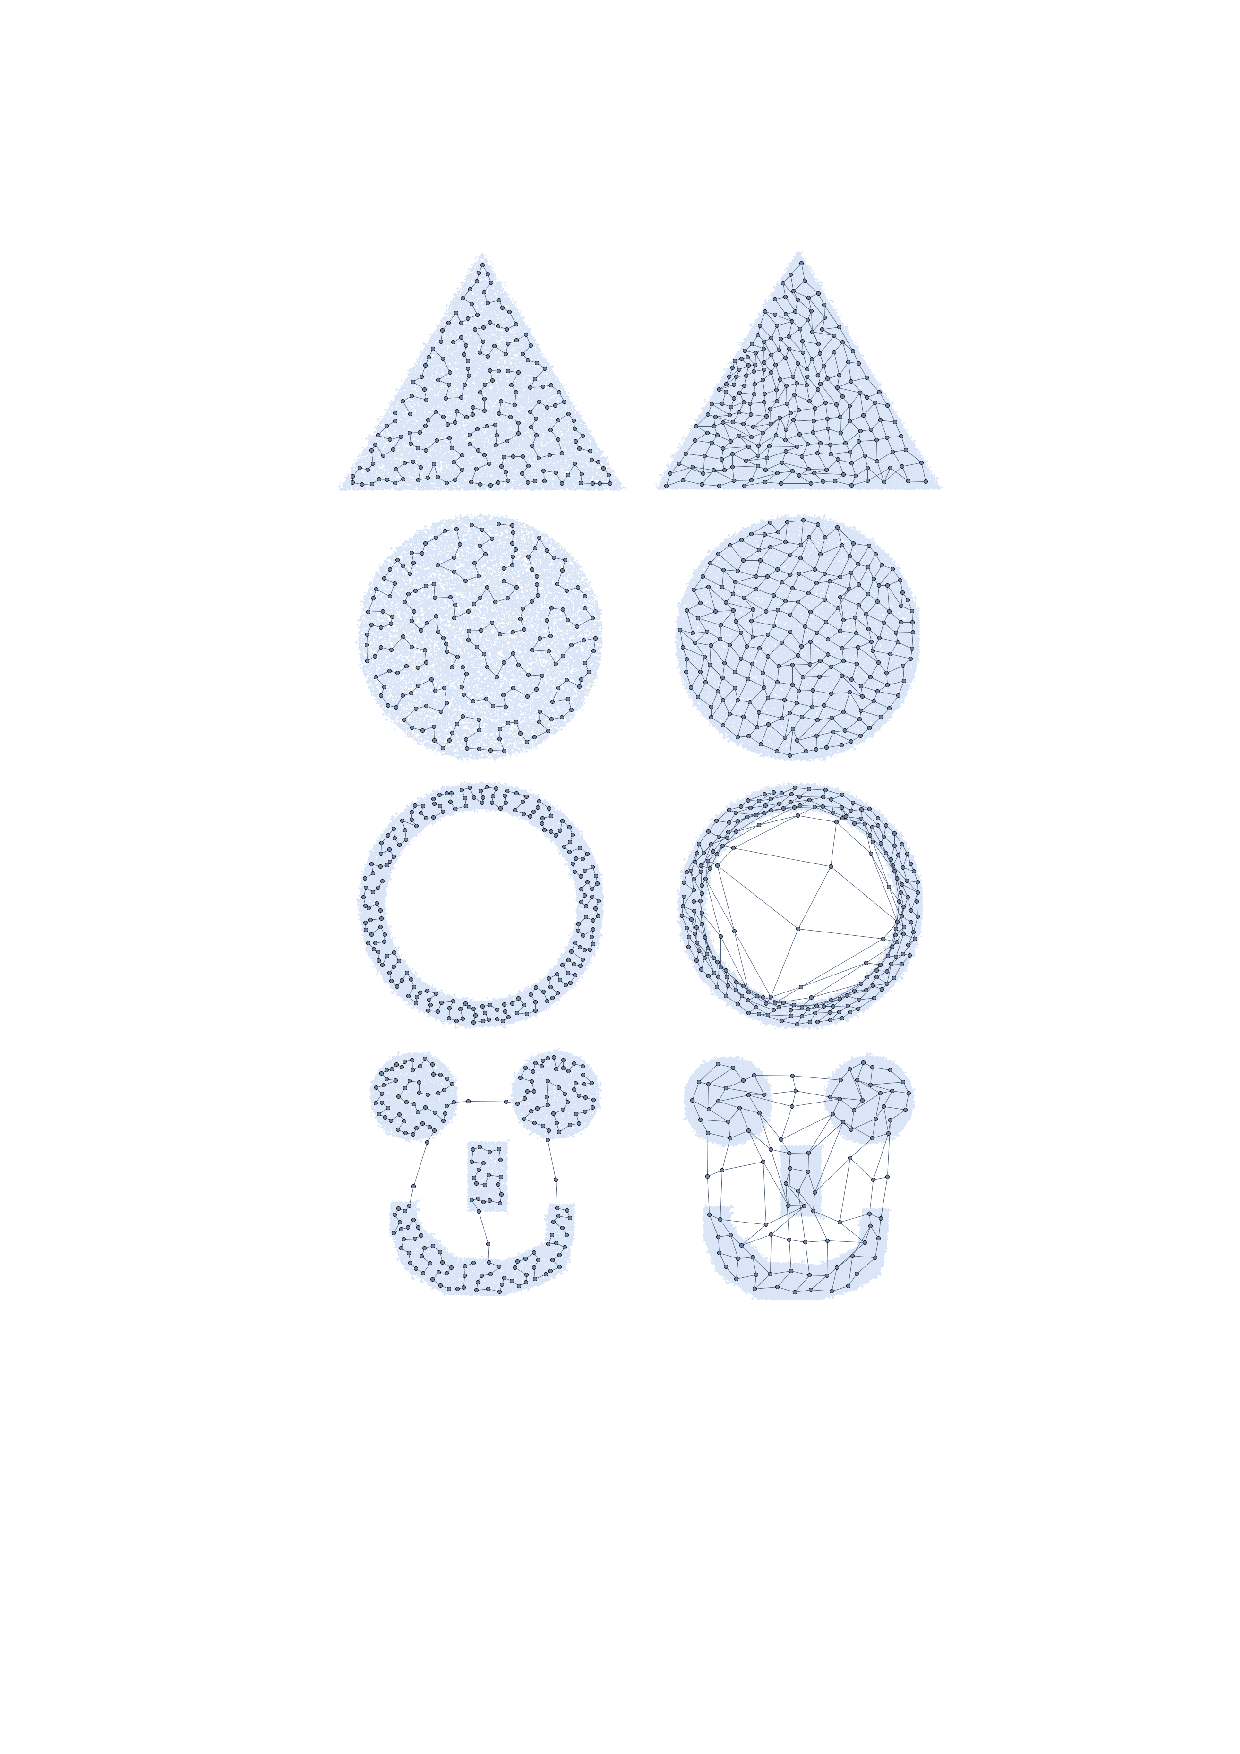
\includegraphics[width=\linewidth]{figures/ch08_som-endzustaende.pdf}
	\caption{Endzustände von eindimensionalen (linke Spalte) und zweidimensionalen (rechte Spalte) SOMs auf verschieden abgedeckten Eingaberäumen. Genutzt wurden bei eindimensionaler Topologie 200 Neuronen, bei zweidimensionaler 10 $\times$ 10 Neurone und bei allen Karten 80.000 Eingabemuster.}
	\label{fig:ch08_som-endzustaende}
\end{figure}



\section{Hopfield-Netze}
% 17
Content here.


\section{Boltzmann-Maschine}
% 18
Ein Problem der Hopfield-Netze ist, dass sie sich häufig in einem lokalen Minimum stabilisieren statt im angestrebten globalen Minimum.
Abhilfe davon schaffen sogenannte statistische Methoden, bei denen die Neuronen ihren Zustand nicht mehr \emph{deterministisch}, sondern \emph{zufällig} nach einer Wahrscheinlichkeitsverteilung ändern.

Die \emph{Boltzmann-Maschine} ist eine solche Methode. Es handelt sich um einen \emph{unüberwachten} Lernalgorithmus, welcher die gleiche rekurrente Netzstruktur wie Hopfield-Netze verwendet. Boltzmann-Maschinen unterscheiden sich jedoch durch eine andere (stochastische) Aktivierungsfunktion und durch ein anderes Lernverfahren.



% ------------------------------------------------------------------------
% ------------------------------------------------------------------------
\section*{Lernverfahren}
Das Lernverfahren der Boltzmann-Maschine hat Ähnlichkeit mit dem technischen Verfahren zum Ausglühen eines Metalls: Zuerst wird das Metall über den Schmelzpunkt erhitzt, danach erfolgt ein langsames Abkühlen (vgl. Abschnitt zu \emph{simulated annealing}).

Bei hohen Temperaturen besitzen die Metallatome \emph{hohe Energien} und können sich nahezu frei bewegen. Dabei werden zufällig alle möglichen Konfigurationen eingenommen. Beim langsamen Abkühlen verringern sich die Energien und das System stabilisiert sich schließlich in einem \emph{Zustand mit minimaler Energie} (globales Minimum der Energiefunktion).
Bei gegebener Temperatur ist die Wahrscheinlichkeitsverteilung der Energie des Systems durch den Boltzmann-Faktor
\[
	e^{(\frac{-E}{kT})}	
\]
gegeben. Dabei sind $E$ die Energie des Systems, $k$ die Boltzmann-Konstante und $T$ die absolute Temperatur.
Für hohe Temperaturen $T$ hat das System eine hohe Wahrscheinlichkeit, hohe Energie zu besitzen. Bei niedrigen Temperaturen $T$ gibt es eine endliche, wenn auch geringe Wahrscheinlichkeit, dass das System trotzdem eine hohe Energie besitzt.


% ------------------------------------------------------------------------
\subsection*{Energie und Aktivierungsfunktion}
Die Energie einer Boltzmann-Maschine wird in gleicher Weise wie bei einem Hopfield-Netz durch die Summe aller paarweisen Energien der Neuronen definiert, üblicherweise nach der Formel
\[
	E = - \sum_{i < j} w_{ij} \cdot o_i \cdot o_j + 
		\sum_i \theta_j \cdot o_j
\]
wobei wie üblich $w_{ij}$ die Verbindung zwischen Neuron $i$ und Neuron $j$, $o_i$ die Ausgabe von Neuron $i$ (entweder 0 oder 1) und $\theta_i$ der Schwellenwert von Neuron $i$ ist.
Aktivierung und Ausgabe einer Zelle sind in diesem Modell identisch, es gilt also $a_j = o_j$.
Man beachte, dass die Summation über alle $i$, $j$ mit $i < j$, d.h. nur über die eine Hälfte der Gewichtsmatrix erfolgt, da die andere \emph{symmetrisch} dazu ist.

Wie bei binären Hopfield-Netzen ist die Energiedifferenz, die durch das Umschalten der Ausgabe eines einzelnen Neurons $k$ entsteht, gegeben durch
\[
	\Delta E_k = net_k - \theta_k = \sum_i (w_{ik} \cdot o_i - \theta_k)
\]

Mit dem \emph{Trick} des "`on"'-Neurons lassen sich die beiden Formeln wie folgt verkürzen:
\begin{align*}
	E &= \sum_{i < j} w_{ij} \cdot o_i \cdot o_j \\
	\Delta E_k &= net_k = \sum_i (w_{ik} \cdot o_i)
\end{align*}


\subsubsection*{Lokale und globale Minima}
Hopfield-Netze sind \emph{deterministische} Algorithmen, die sich entlang des negativen Gradienten dieser Energiefunktion zu einem Minimum bewegen. Dies ist aber in der Regel ein \emph{lokales} und kein globales Minimum.
Um von einem lokalen Minimum zu einem tieferen globalen Minimum zu gelangen, muss man zulassen, dass der Algorithmus nicht immer entlang des Gradienten nach unten geht, sondern gelegentlich auch Gewichtskonfigurationen mit höherer Energie annimmt, um eine \emph{Erhebung zwischen benachbarten Minima zu überwinden}.

Die Boltzmann-Maschine verwendet dazu eine stochastische Aktivierungsfunktion der Neuronen, die von dem bekannten Metropolis-Algorithmus abgeleitet wurde.

Ist  $\Delta E_k$ die Energiedifferenz des Netzes zwischen den beiden Zuständen, bei denen Neuron $k$ den Wert Eins bzw. Null angenommen hat, während alle anderen Neuronen ihre Ausgabe beibehalten haben, so setze die Aktivierung (bzw. Ausgabe) $o_k$ auf $1$ mit der Wahrscheinlichkeit
\[
	p_k = P(o_k \equiv 1) = \underbrace{ \frac{1}{1 + e^{\frac{-\Delta E_k}{T}}}}_{\text{logistische Funktion}}
\]
unabhängig vom früheren Zustand von Neuron $k$. Dies ist eine \emph{stochastische Aktivierungsfunktion}.

Man beachte, dass nicht der \emph{Wert} der Aktivierungsfunktion durch eine Zufallsfunktion bestimmt wird, sondern die Wahrscheinlichkeit, mit der
die Aktivierungsfunktion eine Eins liefert gegenüber einer Null.
Dabei ist $T$ ein künstlicher Temperatur-Parameter, der zuerst auf hohe Werte gesetzt wird und dann im Verlauf des Verfahrens langsam reduziert wird.

Die Aktivierungsfunktion lässt sich damit auch wie folgt schreiben:
\[
	o_k = f_{act}(net_k) = 
	\begin{cases}
		1 &\text{falls } \big( random() \le p_k \big) \\
		0 &\text{sonst}
	\end{cases}
\]

\subsubsection*{Simulated Annealing}
Durch den Temperaturparameter $T$ wird wiederum die Steilheit der logistischen Funktion eingestellt, große Werte von $T$ liefern eine flache Funktion, kleine Werte von $T$ (mit $0 < T < 1$) liefern eine steile Aktivierungsfunktion, die im Grenzfall für $T \rightarrow 0$ gegen die binäre Schwellenwertfunktion konvergiert (siehe Abbildung \ref{fig:ch10_annealing}).

\begin{figure}[ht!] \centering 
	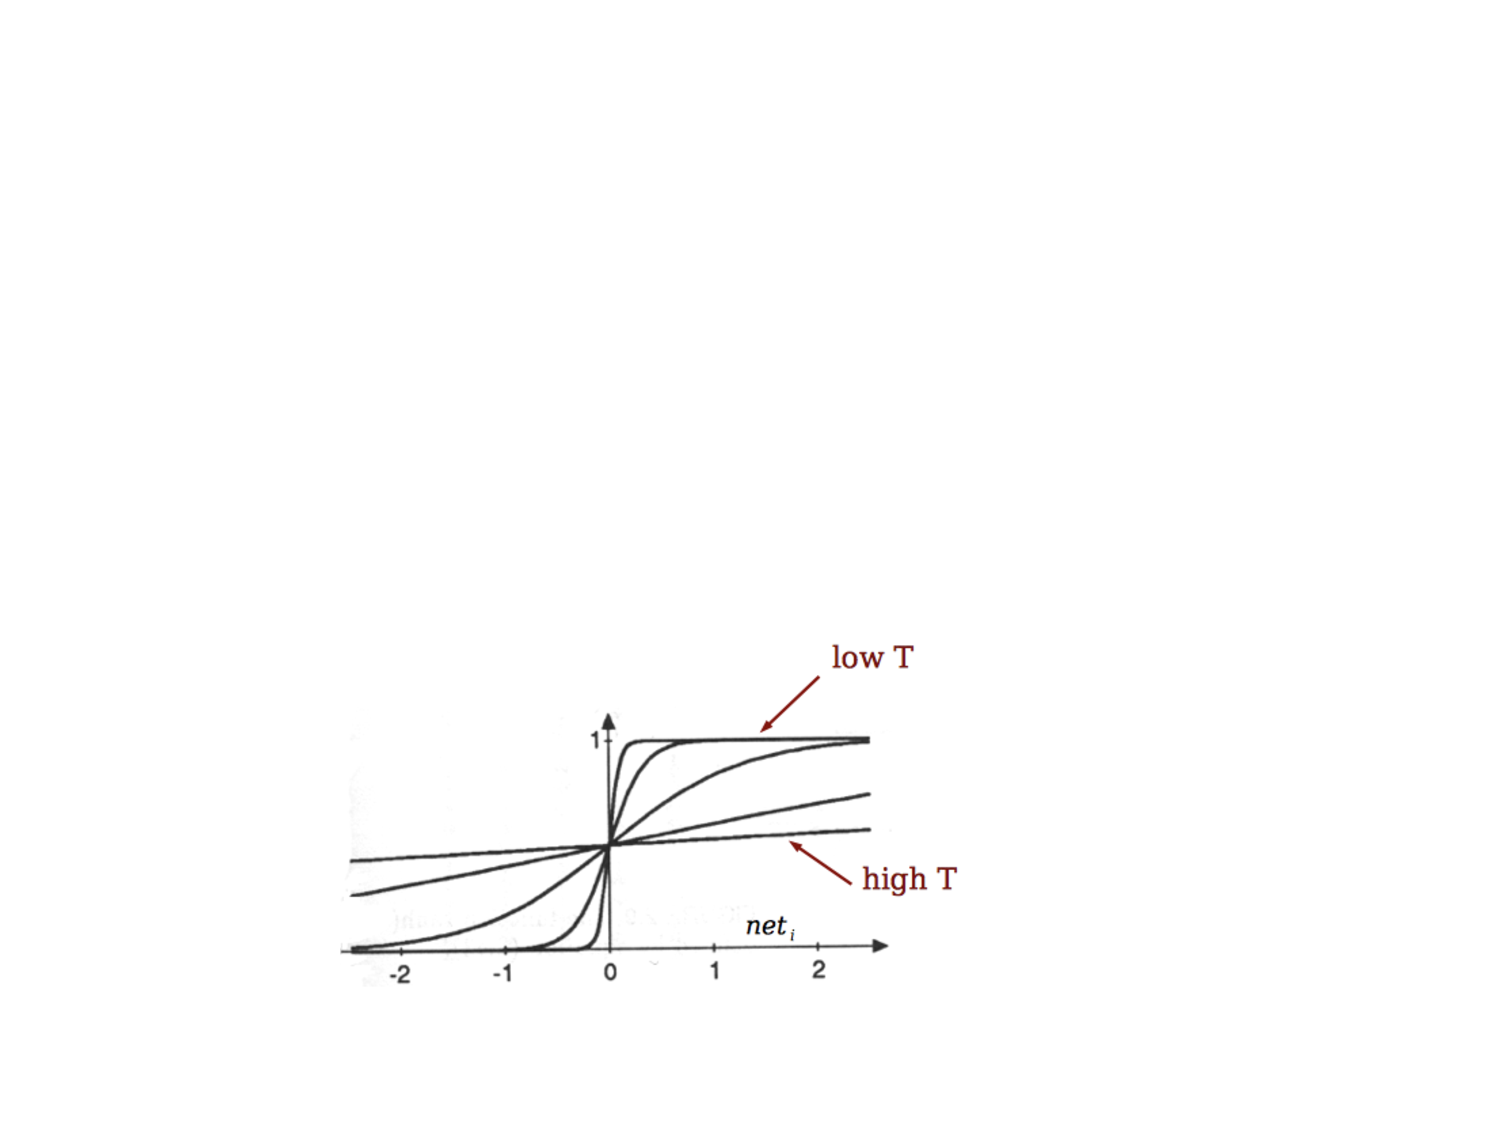
\includegraphics[width=0.7\linewidth]{figures/ch10_annealing.pdf}
	\caption{Logistische Funktion mit verschiedenen Temperaturparametern $T$.}
	\label{fig:ch10_annealing}
\end{figure}

Dieses ermöglicht das sogenannte \emph{simulated annealing}. Dabei wird mit einem großen Wert für $T$ begonnen, um anschließend durch langsames Verkleinern von $T$ ein \emph{Ausglühen} zu simulieren.
So erlaubt man dem Netz zu Beginn mehr Änderungen, was dazu führt, dass es eher aus lokalen Minima herausspringen kann.


% ------------------------------------------------------------------------
\subsection*{Lernregel}
\begin{hint}{Achtung!}{unvollstaendig-search-problem}
	Dieser Abschnitt ist nicht vollständig und muss überarbeitet werden.
\end{hint}
Neuronen einen Boltzmann-Maschine kann man in zwei Gruppen aufteilen:
\begin{enumerate}
	\item sichtbare Neuronen (\emph{visible units}) - Sie sind von außen sichtbar und können von dort Werte erhalten indem ihre Aktivierung, die mit der Ausgabe identisch ist, auf extern vorgegebene Werte $0$ oder $1$ gesetzt wird. 
	\item verdeckte Neuronen (\emph{hidden units}) - Sie sind von außen nicht einsehbar, werden jedoch vom Netzwerk benötigt, um die interne Repräsentation für komplexere Probleme zu bilden. 
\end{enumerate}

Eine beliebige Teilmenge sichtbarer Neuronen kann von außen mit Werten belegt werden. Jeder externe Eingabevektor, der an die sichtbaren Neuronen angelegt wird, wird so lange angelegt, bis sich die Boltzmann-Maschine im Temperaturgleichgewicht stabilisiert hat. Die Struktur der Umgebung kann dann als Wahrscheinlichkeitsverteilung aller $2^v$ Zustände der $v$ sichtbaren Neuronen betrachtet werden.

Ziel des Lernverfahrens der Boltzmann-Maschine ist es nun, die Gewichte des Netzes so anzupassen, dass es genau die gleiche Wahrscheinlichkeitsverteilung auf den sichtbaren Zuständen erreicht ($p(v_{\alpha})$), wie wenn man es im Temperaturgleichgewicht ohne externe Eingaben frei laufen lässt ($\tilde{p}(v_{\alpha})$).


% ------------------------------------------------------------------------
\subsection*{Search Problem}
\begin{hint}{Achtung!}{unvollstaendig-search-problem}
	Dieser Abschnitt ist nicht vollständig und muss überarbeitet werden.
\end{hint}

\begin{figure}[ht!] \centering 
	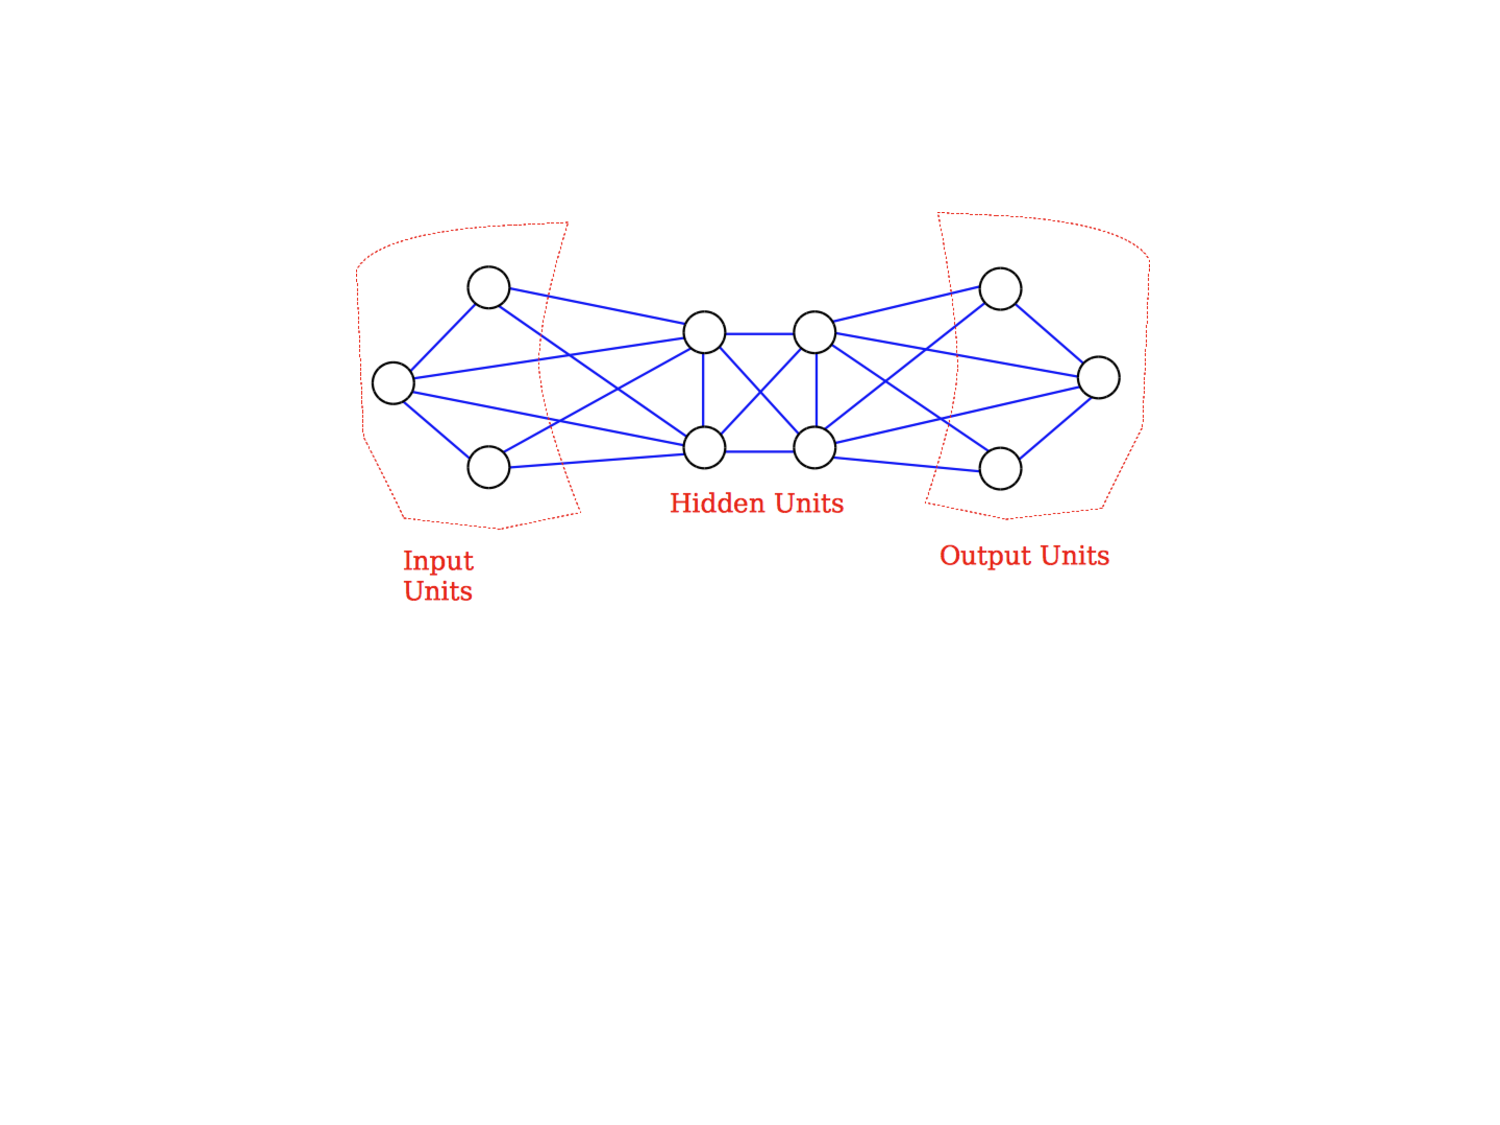
\includegraphics[width=\linewidth]{figures/ch10_boltzmann-search-problem.pdf}
	\caption{Boltzmann-Maschine mit Eingabe- und Ausgabeneuronen, sowie versteckten Neuronen.}
	\label{fig:ch10_boltzmann-search-problem}
\end{figure}



% ------------------------------------------------------------------------
\subsection*{Fazit}
Boltzmann-Maschinen mit ausreichend versteckten Neuronen können jede Funktion berechnen.

Das Training ist aufgrund der komplexen Struktur sehr langsam und rechenintensiv.




% ------------------------------------------------------------------------
% ------------------------------------------------------------------------
\subsection*{Restricted Boltzmann Machines (RBMs)}
\begin{hint}{Achtung!}{unvollstaendig-search-problem}
	Dieser Abschnitt ist nicht vollständig und muss überarbeitet werden.
\end{hint}
Restricted Boltzmann Machines sind die eingeschränkte Variante der Boltzmann-Maschinen. Es handelt sich um ein \emph{unüberwachtes} Lernverfahren, welches automatisch bedeutende Merkmale der Daten extrahiert.

Eine RBM muss dabei ein \emph{bipartiter Graph} sein, wie er in Abbildung \ref{fig:ch10_rbms-bipartiter-graph} dargestellt ist. RBMs bestehen damit aus zwei Schichten: Einer Schicht mit \emph{visible units} und eine mit \emph{hidden units}. 
Die Einschränkung der RBMs ist, dass es keine Kommunikation innerhalb einer Schicht gibt.
Der Vorteil der fehlenden Verbindungen zwischen den versteckten Knoten liegt im \emph{effizienteren} Training.

\begin{figure}[ht!] \centering 
	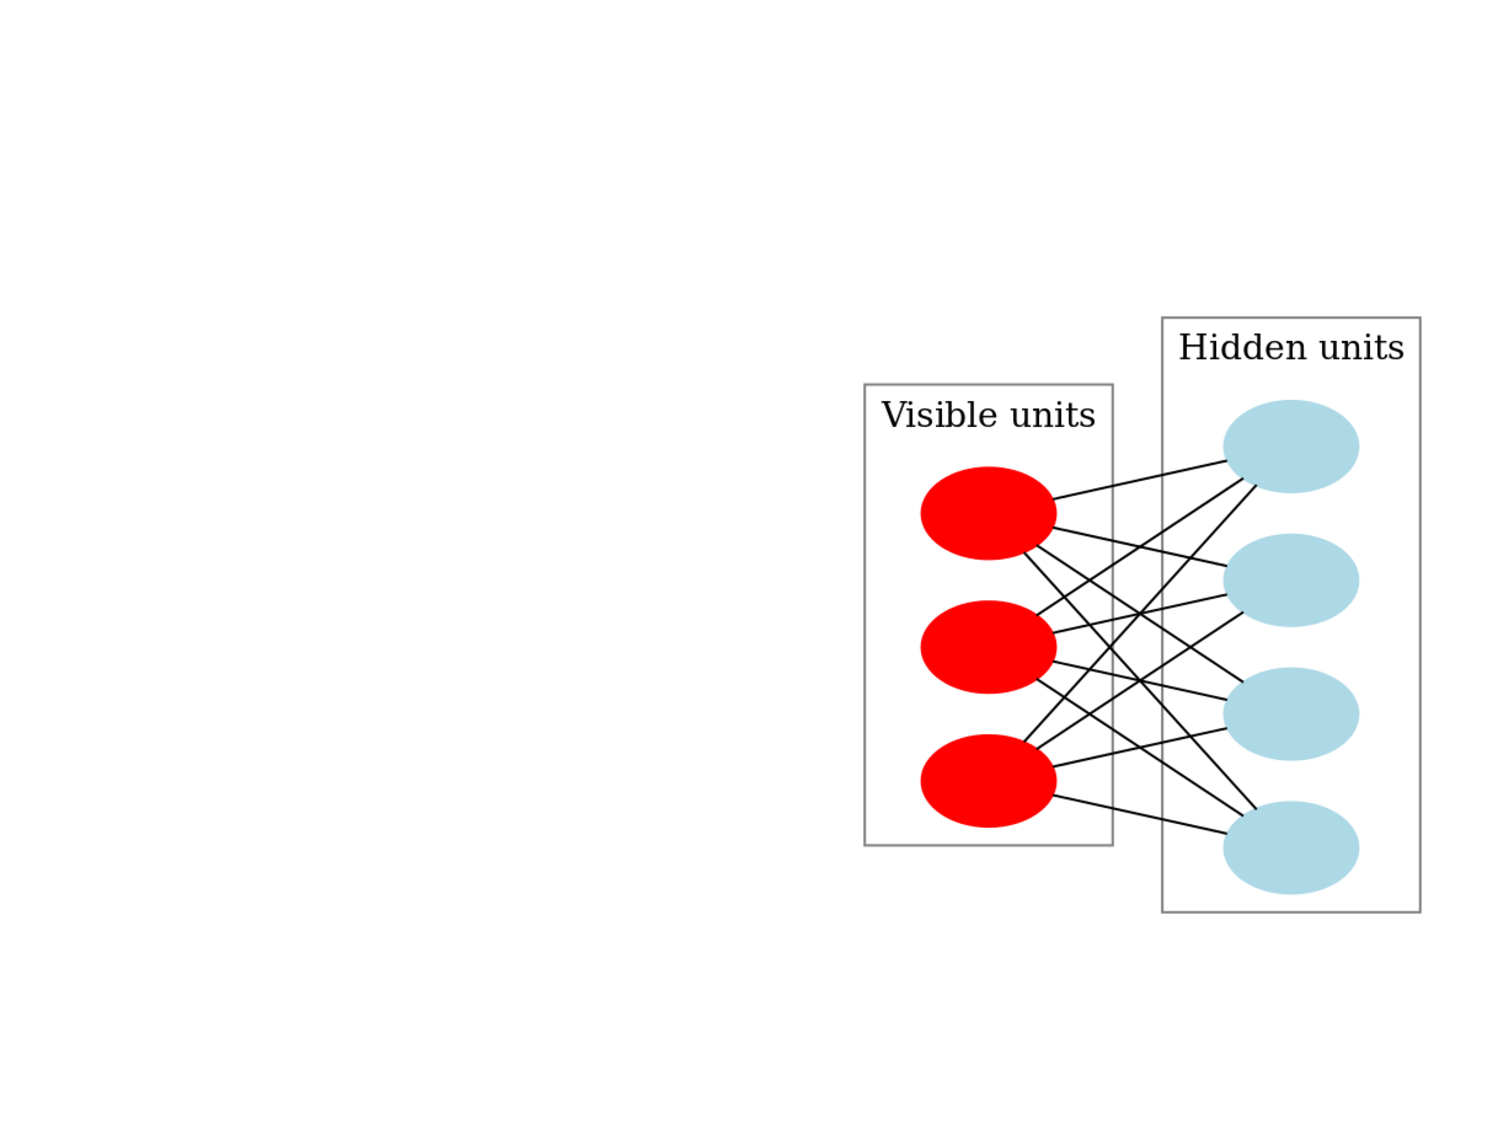
\includegraphics[width=0.5\linewidth]{figures/ch10_rbms-bipartiter-graph.pdf}
	\caption{Restricted Boltzmann-Maschine mit visible und hidden units.}
	\label{fig:ch10_rbms-bipartiter-graph}
\end{figure}

Die Energie $E$ ist definiert durch:
\[
	E(V,H) = - \sum_{i=1}^{m} \sum_{j=1}^{F} w_{ij} h_j v_i + 
		- \sum_{i=1}
\]


\section{Time-Delay-Netze}
% 24
Content here.


\section{Minimierung von NN}
% 25
Content here.


\section{Ausblick/Anwendung neuronaler Netze}
% 40
Content here.


%------------------------------------------------


% Einteilung in den Folien:
% \section{Klassifikation/Mustererkennung}
% \section{Lernende Vektorquantisierung (LVQ) \& Verwandte Techniken}
%\section{Das Perzeptron (+ Biological Neurons)}
%\section{Features}
%\section{Backpropagation}
%\section{Learning Features: Autoencoders and Bottleneck Features}
%\section{Deep Learning}
%\section{Training Neural Networks with Reinforcement Learning}
%\section{Hopfield Nets and Boltzmann Machines}
%\section{Recurrent Neural Networks}
%\section{Deep Learning in Computer Vision}




%----------------------------------------------------------------------------------------
%	REFERENCE LIST
%----------------------------------------------------------------------------------------
\phantomsection
\bibliographystyle{unsrt}
\bibliography{sample}

%----------------------------------------------------------------------------------------

\end{document}